\documentclass[]{book}
\usepackage{lmodern}
\usepackage{amssymb,amsmath}
\usepackage{ifxetex,ifluatex}
\usepackage{fixltx2e} % provides \textsubscript
\ifnum 0\ifxetex 1\fi\ifluatex 1\fi=0 % if pdftex
  \usepackage[T1]{fontenc}
  \usepackage[utf8]{inputenc}
\else % if luatex or xelatex
  \ifxetex
    \usepackage{mathspec}
  \else
    \usepackage{fontspec}
  \fi
  \defaultfontfeatures{Ligatures=TeX,Scale=MatchLowercase}
\fi
% use upquote if available, for straight quotes in verbatim environments
\IfFileExists{upquote.sty}{\usepackage{upquote}}{}
% use microtype if available
\IfFileExists{microtype.sty}{%
\usepackage{microtype}
\UseMicrotypeSet[protrusion]{basicmath} % disable protrusion for tt fonts
}{}
\usepackage[margin=1in]{geometry}
\usepackage{hyperref}
\hypersetup{unicode=true,
            pdftitle={Answering questions with data: Lab Manual},
            pdfauthor={Matthew J. C. Crump; Anajali Krishnan; Stephen Volz; Alla Chavarga; Currently in draft, all attributions and licensed to adapted content will be recognized by the time we are finished.},
            pdfborder={0 0 0},
            breaklinks=true}
\urlstyle{same}  % don't use monospace font for urls
\usepackage{natbib}
\bibliographystyle{apalike}
\usepackage{color}
\usepackage{fancyvrb}
\newcommand{\VerbBar}{|}
\newcommand{\VERB}{\Verb[commandchars=\\\{\}]}
\DefineVerbatimEnvironment{Highlighting}{Verbatim}{commandchars=\\\{\}}
% Add ',fontsize=\small' for more characters per line
\usepackage{framed}
\definecolor{shadecolor}{RGB}{248,248,248}
\newenvironment{Shaded}{\begin{snugshade}}{\end{snugshade}}
\newcommand{\KeywordTok}[1]{\textcolor[rgb]{0.13,0.29,0.53}{\textbf{{#1}}}}
\newcommand{\DataTypeTok}[1]{\textcolor[rgb]{0.13,0.29,0.53}{{#1}}}
\newcommand{\DecValTok}[1]{\textcolor[rgb]{0.00,0.00,0.81}{{#1}}}
\newcommand{\BaseNTok}[1]{\textcolor[rgb]{0.00,0.00,0.81}{{#1}}}
\newcommand{\FloatTok}[1]{\textcolor[rgb]{0.00,0.00,0.81}{{#1}}}
\newcommand{\ConstantTok}[1]{\textcolor[rgb]{0.00,0.00,0.00}{{#1}}}
\newcommand{\CharTok}[1]{\textcolor[rgb]{0.31,0.60,0.02}{{#1}}}
\newcommand{\SpecialCharTok}[1]{\textcolor[rgb]{0.00,0.00,0.00}{{#1}}}
\newcommand{\StringTok}[1]{\textcolor[rgb]{0.31,0.60,0.02}{{#1}}}
\newcommand{\VerbatimStringTok}[1]{\textcolor[rgb]{0.31,0.60,0.02}{{#1}}}
\newcommand{\SpecialStringTok}[1]{\textcolor[rgb]{0.31,0.60,0.02}{{#1}}}
\newcommand{\ImportTok}[1]{{#1}}
\newcommand{\CommentTok}[1]{\textcolor[rgb]{0.56,0.35,0.01}{\textit{{#1}}}}
\newcommand{\DocumentationTok}[1]{\textcolor[rgb]{0.56,0.35,0.01}{\textbf{\textit{{#1}}}}}
\newcommand{\AnnotationTok}[1]{\textcolor[rgb]{0.56,0.35,0.01}{\textbf{\textit{{#1}}}}}
\newcommand{\CommentVarTok}[1]{\textcolor[rgb]{0.56,0.35,0.01}{\textbf{\textit{{#1}}}}}
\newcommand{\OtherTok}[1]{\textcolor[rgb]{0.56,0.35,0.01}{{#1}}}
\newcommand{\FunctionTok}[1]{\textcolor[rgb]{0.00,0.00,0.00}{{#1}}}
\newcommand{\VariableTok}[1]{\textcolor[rgb]{0.00,0.00,0.00}{{#1}}}
\newcommand{\ControlFlowTok}[1]{\textcolor[rgb]{0.13,0.29,0.53}{\textbf{{#1}}}}
\newcommand{\OperatorTok}[1]{\textcolor[rgb]{0.81,0.36,0.00}{\textbf{{#1}}}}
\newcommand{\BuiltInTok}[1]{{#1}}
\newcommand{\ExtensionTok}[1]{{#1}}
\newcommand{\PreprocessorTok}[1]{\textcolor[rgb]{0.56,0.35,0.01}{\textit{{#1}}}}
\newcommand{\AttributeTok}[1]{\textcolor[rgb]{0.77,0.63,0.00}{{#1}}}
\newcommand{\RegionMarkerTok}[1]{{#1}}
\newcommand{\InformationTok}[1]{\textcolor[rgb]{0.56,0.35,0.01}{\textbf{\textit{{#1}}}}}
\newcommand{\WarningTok}[1]{\textcolor[rgb]{0.56,0.35,0.01}{\textbf{\textit{{#1}}}}}
\newcommand{\AlertTok}[1]{\textcolor[rgb]{0.94,0.16,0.16}{{#1}}}
\newcommand{\ErrorTok}[1]{\textcolor[rgb]{0.64,0.00,0.00}{\textbf{{#1}}}}
\newcommand{\NormalTok}[1]{{#1}}
\usepackage{longtable,booktabs}
\usepackage{graphicx,grffile}
\makeatletter
\def\maxwidth{\ifdim\Gin@nat@width>\linewidth\linewidth\else\Gin@nat@width\fi}
\def\maxheight{\ifdim\Gin@nat@height>\textheight\textheight\else\Gin@nat@height\fi}
\makeatother
% Scale images if necessary, so that they will not overflow the page
% margins by default, and it is still possible to overwrite the defaults
% using explicit options in \includegraphics[width, height, ...]{}
\setkeys{Gin}{width=\maxwidth,height=\maxheight,keepaspectratio}
\IfFileExists{parskip.sty}{%
\usepackage{parskip}
}{% else
\setlength{\parindent}{0pt}
\setlength{\parskip}{6pt plus 2pt minus 1pt}
}
\setlength{\emergencystretch}{3em}  % prevent overfull lines
\providecommand{\tightlist}{%
  \setlength{\itemsep}{0pt}\setlength{\parskip}{0pt}}
\setcounter{secnumdepth}{5}
% Redefines (sub)paragraphs to behave more like sections
\ifx\paragraph\undefined\else
\let\oldparagraph\paragraph
\renewcommand{\paragraph}[1]{\oldparagraph{#1}\mbox{}}
\fi
\ifx\subparagraph\undefined\else
\let\oldsubparagraph\subparagraph
\renewcommand{\subparagraph}[1]{\oldsubparagraph{#1}\mbox{}}
\fi

%%% Use protect on footnotes to avoid problems with footnotes in titles
\let\rmarkdownfootnote\footnote%
\def\footnote{\protect\rmarkdownfootnote}

%%% Change title format to be more compact
\usepackage{titling}

% Create subtitle command for use in maketitle
\newcommand{\subtitle}[1]{
  \posttitle{
    \begin{center}\large#1\end{center}
    }
}

\setlength{\droptitle}{-2em}

  \title{Answering questions with data: Lab Manual}
    \pretitle{\vspace{\droptitle}\centering\huge}
  \posttitle{\par}
    \author{Matthew J. C. Crump \\ Anajali Krishnan \\ Stephen Volz \\ Alla Chavarga \\ Currently in draft, all attributions and licensed to adapted content
will be recognized by the time we are finished.}
    \preauthor{\centering\large\emph}
  \postauthor{\par}
      \predate{\centering\large\emph}
  \postdate{\par}
    \date{2018: Last Compiled 2018-07-26}

\usepackage{booktabs}
\usepackage{amsthm}
\makeatletter
\def\thm@space@setup{%
  \thm@preskip=8pt plus 2pt minus 4pt
  \thm@postskip=\thm@preskip
}
\makeatother

\usepackage{amsthm}
\newtheorem{theorem}{Theorem}[chapter]
\newtheorem{lemma}{Lemma}[chapter]
\theoremstyle{definition}
\newtheorem{definition}{Definition}[chapter]
\newtheorem{corollary}{Corollary}[chapter]
\newtheorem{proposition}{Proposition}[chapter]
\theoremstyle{definition}
\newtheorem{example}{Example}[chapter]
\theoremstyle{definition}
\newtheorem{exercise}{Exercise}[chapter]
\theoremstyle{remark}
\newtheorem*{remark}{Remark}
\newtheorem*{solution}{Solution}
\begin{document}
\maketitle

{
\setcounter{tocdepth}{1}
\tableofcontents
}
\chapter*{Preface}\label{preface}
\addcontentsline{toc}{chapter}{Preface}

\begin{center}
\includegraphics[width=12.5in]{LabmanualCover} \end{center}

This lab manual involves tutorials and data-analysis problems using the
free statistics software R, as well as Excel, and SPSS. The goal is to
train students to be able to organize and analyze data common to
research in psychology, as well as to understand the ideas behind the
analyses so students can take creative approaches to answering questions
with data.

\section{R}\label{r}

\includegraphics[width=1.39in]{figures/rlogo}

R is primarily a computer programming language for statistical analysis.
It is \emph{free}, and \emph{open-source} (many people contribute to
developing it), and runs on most operating systems. It is a powerful
language that can be used for all sorts of mathematical operations,
data-processing, analysis, and graphical display of data. I even used R
to write this lab manual. And, I use R all the time for my own research,
because it makes data-analyis fast, efficient, transparent,
reproducible, and exciting.

Statistics Software

\begin{itemize}
\tightlist
\item
  \href{http://www-01.ibm.com/software/analytics/spss/}{SPSS}
\item
  \href{http://www.sas.com/en_us/home.html}{SAS}
\item
  \href{http://www.jmp.com}{JMP}
\item
  \href{http://www.r-project.org}{R}
\item
  \href{http://julialang.org}{Julia}
\item
  \href{http://www.mathworks.com/products/matlab/}{Matlab}
\end{itemize}

\section{Why R?}\label{why-r}

There are lots of different options for using computers to analyze data,
why use R?. The options all have pros and cons, and can be used in
different ways to solve a range of different problems. Some software
allows you to load in data, and then analyze the data by clicking
different options in a menu. This can sometimes be fast and convenient.
For example, once the data is loaded, all you have to do is click a
couple buttons to analyse the data! However, many aspects of
data-analysis are not so easy. For example, usually particular analyses
require that the data be formatted in a particular way so that the
program analyze it properly. Often times when a researcher wants to ask
a new question of an existing data set, they have to spend time
re-formatting the data. If the data is large, then reformattin by hand
is very slow, and can lead to errors. Another option, is to use a
scripting language to instruct the computer how reformat the data. This
is very fast and efficient. R provides the ability to everything all in
one place. You can load in data, reformat it any way you like, then
anlayze it anyway you like, and create beautiful graphs and tables
(publication quality) to display your findings. Once you get the hang of
R, it becomes very fast and efficient.

\section{Installing R and R Studio}\label{installing-r-and-r-studio}

Download and install R onto your computer. The R website is:
\url{http://www.r-project.org}

Find the download R using the link. This will take you to a page with
many different mirror links. You can click any of these links to
download a version of R that will work on your computer. After you have
installed R you can continue.

After you have installed R on your computer, you should want to install
another program called R studio. This program provides a user-friendly
interface for using R. You must already have installed R before you
perform this step. The R-studio website is: \url{http://www.rstudio.com}

Find the download link on the front-page, and then download R studio
desktop version for your computer. After you have installed R studio you
will be ready to start using R.

The website \href{http://www.r-fiddle.org}{R-fiddle} allows you to run R
scripts in the cloud, so you can practice R from your web-browser!

\section{R studio notes and tips}\label{r-studio-notes-and-tips}

\begin{figure}[htbp]
\centering
\includegraphics{figures/FigRstudio.pdf}
\caption{\label{fig:2rstudiod}The R-studio workspace}
\end{figure}

\subsection{Console}\label{console}

When you open up R studio you will see three or four main windows (the
placement of each are configurable). In the above example, the bottom
left window is the command line (terminal or console) for R. This is
used to directly enter commands into R. Once you have entered a command
here, press enter to execute the command. The console is useful for
entering single lines of code and running them. Oftentimes this occurs
when you are learning how to correctly execute a line of code in R. Your
first few attempts may be incorrect resulting in errors, but trying out
different variations on your code in the command line can help you
produce the correct code. Pressing the up arrow while in the console
will scroll through the most recently executed lines of code.

\subsection{Script Editor}\label{script-editor}

The top left corner contains the script editor. This is a simple text
editor for writing and saving R scripts with many lines. Several tabs
can be opened at once, with each tab representing a different R script.
R scripts can be saved from the editor (resulting in a .r file). Whole
scripts can be run by copy and pasting them into the console and
pressing enter. Alternatively, you can highlight portions of the script
that you want to run (in the script editor) and press command-enter to
automatically run that portion in the console (or press the button for
running the current line/section: green arrow pointing right).

\subsection{Workspace and History}\label{workspace-and-history}

The top right panel contains two tabs, one for the workspace and another
for history. The workspace lists out all of the variables and functions
that are currently loaded in R's memory. You can inspect each of the
variables by clicking on them. This is generally only useful for
variables that do not contain large amounts of information. The history
tab provides a record of the recent commands executed in the console.

\subsection{File, Plot, Packages, Help}\label{file-plot-packages-help}

The bottom-right window has four tabs for files, plots, packages, and
help. The files tab allows browsing of the computers file directory. An
important concept in R is the \textbf{current working directory}. This
is file folder that R points to by default. Many functions in R will
save things directly to this direct, or attempt to read files from this
directory. The current working directory can be changed by navigating to
the desired folder in the file menu, and then clicking on the more
option to set that folder to the current working directory. This is
especially important when reading in data to R. The current working
directory should be set to the folder containing the data to be inputted
into R. The plots tab will show recent plots and figures made in R. The
packages tab lists the current R libraries loaded into memory, and
provides the ability to download and enable new R packages. The help
menu is an invaluable tool. Here, you can search for individual R
commands to see examples of how they are used. Sometimes the help files
for individual commands are opaque and difficult to understand, so it is
necessary to do a google search to find better examples of using these
commands.

\section{Final comments}\label{final-comments}

In this course we will be using R as a tool to analyze data, and as a
tool to help us gain a better understanding of what our analyses are
doing. Throughout each lab we will show you how to use R to solve
specific problems, and then you will use the examples to solve homework
and lab assignments. R is a very deep programming language, and in many
ways we will only be skimming the surface of what R can do. Along the
way, there will be many pointers to more advanced techniques that
interested students can follow to become experts in using R for
data-analysis, and computer programming in general.

\chapter{Lab 1: Graphing Data}\label{lab-1-graphing-data}

{ The commonality between science and art is in trying to see profoundly
- to develop strategies of seeing and showing. ---Edward Tufte }

As we have found out from the textbook and lecture, when we measure
things, we get lots of numbers. Too many. Sometimes so many your head
explodes just thinking about them. One of \textbf{the most helpful
things} you can do to begin to make sense of these numbers, is to look
at them in graphical form. Unfortunately, for sight-impaired
individuals, graphical summary of data is much more well-developed than
other forms of summarizing data for our human senses. Some researchers
are developing auditory versions of visual graphs, a process called
\textbf{sonification}, but we aren't prepared to demonstrate that here.
Instead, we will make charts, and plots, and things to look at, rather
than the numbers themselves, mainly because these are tools that are
easiest to get our hands on, they are the most developed, and they work
really well for visual summary. If time permits, at some point I would
like to come back here and do the same things with sonification. I think
that would be really, really cool!

\section{General Goals}\label{general-goals}

Our general goals for this first lab are to get your feet wet, so to
speak. We'll do these things:

\begin{enumerate}
\def\labelenumi{\arabic{enumi}.}
\tightlist
\item
  Load in some data to a statistical software program
\item
  Talk a little bit about how the data is structured
\item
  Make graphs of the data so we can look at it and make sense of it.
\end{enumerate}

\section{R}\label{r-1}

Your lab instructor will show you how to open R-studio on the lab
computer. Just find it and double-click. Now you have R-studio.

There are numerous resources for learning about R, we put some of them
on the course website, under the
\href{https://crumplab.github.io/psyc3400/Resources.html}{resouces
page}. You will find these resources helpful as you learn. We also have
a kind of \href{}{general introduction to R and Rstudio here}. This
shows you how to download R and R-studio at home (it's free).

When we made this course, we assumed that most students would be
unfamiliar with R and R-studio, and might even be frightened of it,
because it is a computer programming language (OOOOHHH NOOOOOOO, I NEED
TO DROP THIS COURSE NOW)\ldots{}Don't worry. It's going to be way easier
than you think. Let's compare to other statistics courses where you
would learn something like SPSS. That is also a limited programming
language, but you would mostly learn how to point with a mouse, and
click with button. I bet you already know how to do that. I bet you also
already know how to copy and paste text, and press enter. That's mostly
what we'll be doing to learn R. We will be doing statistics by typing
commands, rather than by clicking buttons. However, lucky for you, all
of the commands are already written for you. You just have to copy/paste
them.

We know that this will seem challenging at first. But, we think that
with lots of working examples, you will get the hang of it, and by the
end of the course you will be able to do things you might never have
dreamed you can do. It's really a fantastic skill to learn, even if you
aren't planning on going on to do research in Psychology (in which case,
this kind of thing is necessary skill to learn). With that, let's begin.

\subsection{Get some data}\label{get-some-data}

In order to graph data, we need to have some data first\ldots{}Actually,
with R, that's not quite true. Run this bit of code and see what
happens:

\begin{Shaded}
\begin{Highlighting}[]
\KeywordTok{hist}\NormalTok{(}\KeywordTok{rnorm}\NormalTok{(}\DecValTok{100}\NormalTok{, }\DataTypeTok{mean=}\DecValTok{50}\NormalTok{, }\DataTypeTok{sd=}\DecValTok{25}\NormalTok{))}
\end{Highlighting}
\end{Shaded}

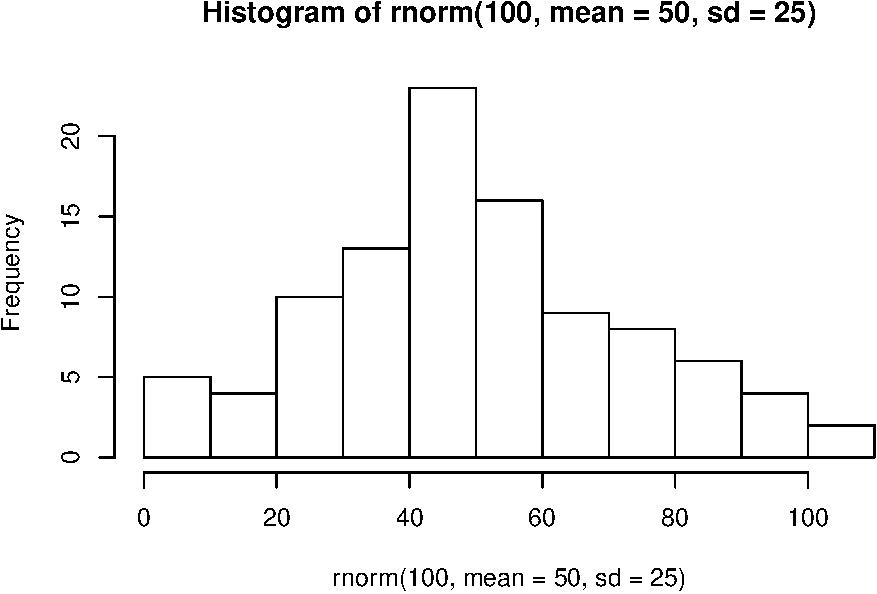
\includegraphics{Programming_Crump_files/figure-latex/unnamed-chunk-2-1.pdf}

You just made R sample 100 numbers, and then plot the results in a
histogram. Pretty neat. We'll be doing some of this later in the course,
where get R to make fake data for us, and then we learn to think about
how data behaves under different kinds of assumptions.

For now, let's do something that might be a little bit more
interesting\ldots{}what movies are going to be filming in NYC? It turns
out that NYC makes a lot of data about a lot things open and free for
anyone to download and look at. This is the NYC Open Data website:
\url{https://opendata.cityofnewyork.us}. I searched through the data,
and found this data file that lists the locations of film permits for
shooting movies all throughout the burroughs. You can download the data
to your computer from
\href{https://raw.githubusercontent.com/CrumpLab/statisticsLab/master/data/MehrSongSpelke2016.csv}{this
link}

NOTE TO SELF, COME BACK HERE AND WALKTHROUGH FILE PATHS AND THINGS

\begin{Shaded}
\begin{Highlighting}[]
\KeywordTok{library}\NormalTok{(data.table)}
\NormalTok{nyc_films <-}\KeywordTok{fread}\NormalTok{(}\StringTok{"data/Film_Permits.csv"}\NormalTok{)}
\end{Highlighting}
\end{Shaded}

\subsection{Look at the data}\label{look-at-the-data}

You will be downloading and analyzing all kinds of data files this
semester. We will follow the very same steps every time. The steps are
to load the data, then look at it. You want to see what you've got.

In R-studio, you will now see a variable called \texttt{nyc\_films} in
the top right-hand corner of the screen, in the environment tab. If you
click this thing, it will show you the contents of the data in a new
window. The data is stored in something we call a \texttt{data\ frame}.
It's R lingo, for the thing that contains the data. Notice is a square,
with rows going across, and columns going up and down. It looks kind of
like an excel spreadsheet if you are familiar with Excel.

It's useful to know you can look at the data frame this way if you need
to. But, this dataframe is really big, it has 50,728 rows of data.
That's a lot too much to look at.

\subsubsection{summarytools}\label{summarytools}

The summarytools packages give a quick way to summarize all of the data
in a data frame. Here's how. When you run this code you will see the
summary in the viewer on the bottom right hand side. There's a little
browser button (arrow on top of little window) that you can click to
expand and see the whole thing in a browser.

\begin{Shaded}
\begin{Highlighting}[]
\KeywordTok{library}\NormalTok{(summarytools)}
\KeywordTok{view}\NormalTok{(}\KeywordTok{dfSummary}\NormalTok{(nyc_films))}
\end{Highlighting}
\end{Shaded}

That is super helpful, but it's still a lot to look at. Because there is
so much data here, it's pretty much mind-boggling to start thinking
about what to do with it.

\subsection{Make Plots to answer
questions}\label{make-plots-to-answer-questions}

Let's walk through a couple questions we might have about this data. We
can see that there were 50,728 film permits made. We can also see that
there are different columns telling us information about each of the
film permits. For example, the \texttt{Borough} column lists the Borough
for each request, whether it was made for: Manhattan, Brooklyn, Bronx,
Queen's, or Staten Island. Now we can ask our first question, and learn
how to do some plotting in R.

\subsubsection{Where are the most film permits being
requested?}\label{where-are-the-most-film-permits-being-requested}

Do you have any guesses? Is it Manhattan, or Brookyln, of the Bronx? Or
Queen's or Staten Island? We can find out by plotting the data using a
bar plot. We just need to count how many film permits are made in each
burough, and then make different bars represent the the counts.

First, we do the counting in R. Run the following code.

\begin{Shaded}
\begin{Highlighting}[]
\KeywordTok{library}\NormalTok{(dplyr)}

\NormalTok{counts <-}\StringTok{ }\NormalTok{nyc_films %>%}
\StringTok{          }\KeywordTok{group_by}\NormalTok{(Borough) %>%}
\StringTok{          }\KeywordTok{summarize}\NormalTok{(}\DataTypeTok{count_of_permits =} \KeywordTok{length}\NormalTok{(Borough))}
\end{Highlighting}
\end{Shaded}

The above grouped the data by each of the five Borough's, and then
counted the number of times each Borough occured (using the
\texttt{length} function). The result is a new variable called
\texttt{count}. I chose to name this variable \texttt{count}. You can
see that it is now displayed in the top-right hand corned in the
environment tab. If you gave \texttt{count} a different name, like
\texttt{muppets}, then it would be named what you called it.

If you click on the \texttt{counts} variable, you will see the five
boroughs listed, along with the counts for how many film permits were
requested in each Borough. These are the numbers that we want to plot in
a graph.

We do the plot using a fantastic package called \texttt{ggplot2}. It is
very powerful once you get the hand of it, and when you do, you will be
able to make all sorts of interesting graphs. Here's the code to make
the plot

\begin{Shaded}
\begin{Highlighting}[]
\KeywordTok{library}\NormalTok{(ggplot2)}

\KeywordTok{ggplot}\NormalTok{(counts, }\KeywordTok{aes}\NormalTok{(}\DataTypeTok{x =} \NormalTok{Borough, }\DataTypeTok{y =} \NormalTok{count_of_permits )) +}
\StringTok{  }\KeywordTok{geom_bar}\NormalTok{(}\DataTypeTok{stat=}\StringTok{"identity"}\NormalTok{)}
\end{Highlighting}
\end{Shaded}

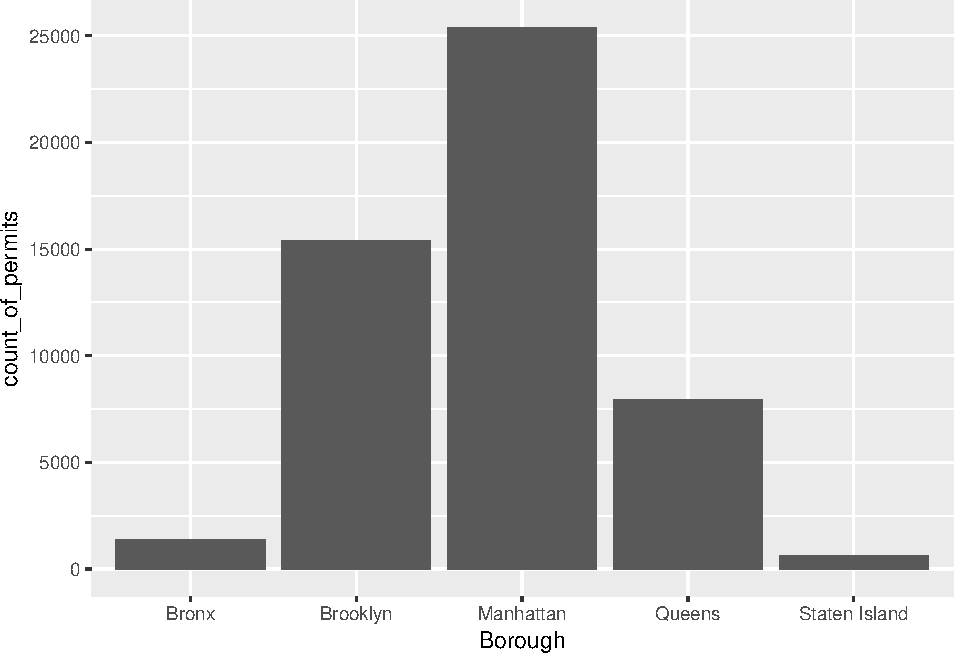
\includegraphics{Programming_Crump_files/figure-latex/unnamed-chunk-6-1.pdf}

There it is, we're done here! We can easily look at this graph, and
answer our question. Most of the film permits were requested in
Manhattan, followed by Brooklyn, then Queen's, the Bronx, and finally
Staten Island.

\subsubsection{\texorpdfstring{What kind of ``films'' are being made,
what is the
category?}{What kind of films are being made, what is the category?}}\label{what-kind-of-films-are-being-made-what-is-the-category}

We think you might be skeptical of what you are doing here, copying and
pasting things. Soon you'll see just how fast you can do things by
copying and pasting, and make a few little changes. Let's quickly ask
another question about what kinds of films are being made. The column
\texttt{Category}, gives us some information about that. Let's just copy
paste the code we already made, and see what kinds of categories the
films fall into. See if you can tell what I changed in the code to make
this work, I'll do it all at once:

\begin{Shaded}
\begin{Highlighting}[]
\NormalTok{counts <-}\StringTok{ }\NormalTok{nyc_films %>%}
\StringTok{          }\KeywordTok{group_by}\NormalTok{(Category) %>%}
\StringTok{          }\KeywordTok{summarize}\NormalTok{(}\DataTypeTok{count_of_permits =} \KeywordTok{length}\NormalTok{(Category))}

\KeywordTok{ggplot}\NormalTok{(counts, }\KeywordTok{aes}\NormalTok{(}\DataTypeTok{x =} \NormalTok{Category, }\DataTypeTok{y =} \NormalTok{count_of_permits )) +}
\StringTok{  }\KeywordTok{geom_bar}\NormalTok{(}\DataTypeTok{stat=}\StringTok{"identity"}\NormalTok{)+}\StringTok{ }
\StringTok{  }\KeywordTok{theme}\NormalTok{(}\DataTypeTok{axis.text.x =} \KeywordTok{element_text}\NormalTok{(}\DataTypeTok{angle =} \DecValTok{90}\NormalTok{, }\DataTypeTok{hjust =} \DecValTok{1}\NormalTok{))}
\end{Highlighting}
\end{Shaded}

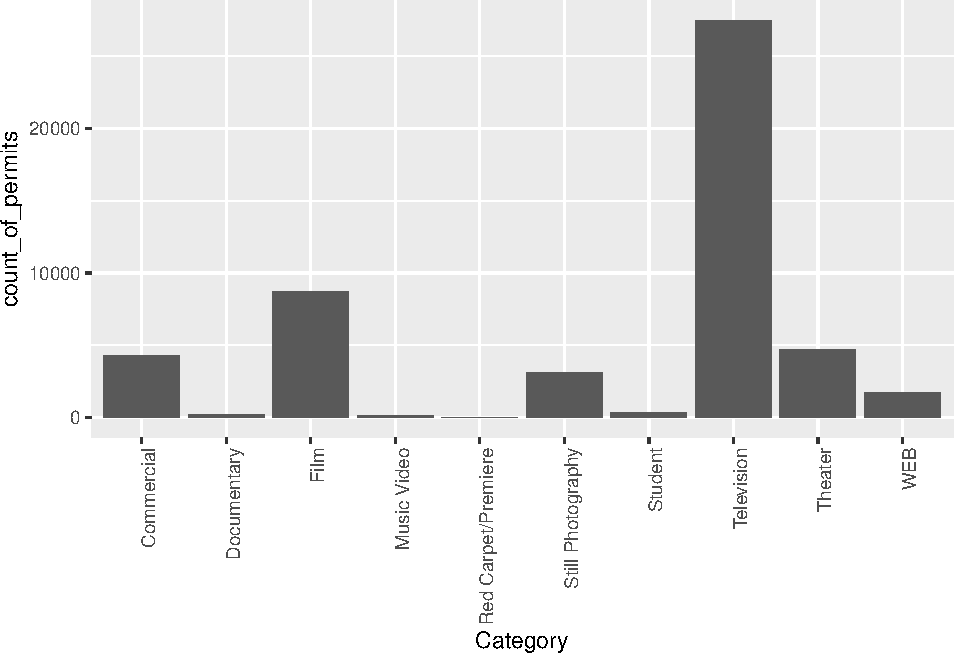
\includegraphics{Programming_Crump_files/figure-latex/unnamed-chunk-7-1.pdf}

Ok, so this figure might look a bit weird because the labels on the
bottom are running into each other. We'll fix that in a bit. First,
let's notice the changes.

\begin{enumerate}
\def\labelenumi{\arabic{enumi}.}
\item
  I changed \texttt{Borough} to \texttt{Category}. That was the main
  thing
\item
  I left out a bunch of things from before. None of the
  \texttt{library()} commands are used again, and I didn't re-run the
  very early code to get the data. R already has those things in it's
  memory, so we don't need to do that first. If you ever clear the
  memory of R, then you will need to reload those things. First-things
  come first.
\end{enumerate}

Fine, so how do we fix the graph? Good question. To be honest, I don't
know right now. I totally forgot how. But, I know ggplot2 can do this,
and I'm going to google it, right now. Then I'm going to find the
answer, and use it here. The googling of your questions is a fine way to
learn. It's what everybody does these days\ldots{}.{[}goes to
google\ldots{}{]}.

Found it, actually found a lot of ways to do this. The trick is to add
the last line. I just copy-pasted it from the solution I found on
\href{https://stackoverflow.com/questions/1330989/rotating-and-spacing-axis-labels-in-ggplot2}{stack
overflow} (you will become friend's with stack overflow, there are many
solutions there to all of your questions)

\begin{Shaded}
\begin{Highlighting}[]
\NormalTok{counts <-}\StringTok{ }\NormalTok{nyc_films %>%}
\StringTok{          }\KeywordTok{group_by}\NormalTok{(Category) %>%}
\StringTok{          }\KeywordTok{summarize}\NormalTok{(}\DataTypeTok{count_of_permits =} \KeywordTok{length}\NormalTok{(Category))}

\KeywordTok{ggplot}\NormalTok{(counts, }\KeywordTok{aes}\NormalTok{(}\DataTypeTok{x =} \NormalTok{Category, }\DataTypeTok{y =} \NormalTok{count_of_permits )) +}
\StringTok{  }\KeywordTok{geom_bar}\NormalTok{(}\DataTypeTok{stat=}\StringTok{"identity"}\NormalTok{)+}\StringTok{ }
\StringTok{  }\KeywordTok{theme}\NormalTok{(}\DataTypeTok{axis.text.x =} \KeywordTok{element_text}\NormalTok{(}\DataTypeTok{angle =} \DecValTok{90}\NormalTok{, }\DataTypeTok{hjust =} \DecValTok{1}\NormalTok{))}
\end{Highlighting}
\end{Shaded}

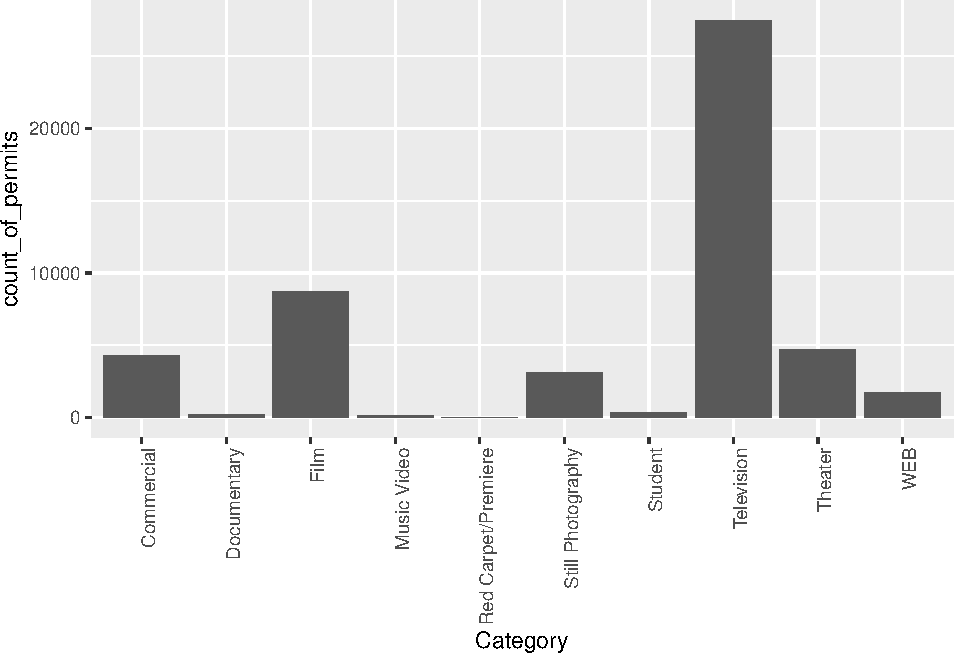
\includegraphics{Programming_Crump_files/figure-latex/unnamed-chunk-8-1.pdf}

\subsection{ggplot2 basics}\label{ggplot2-basics}

Before we go further, I want to point out some basic properties of
ggplot2, just to give you a sense of how it is working. This will make
more sense in a few weeks, so come back here to remind yourself. We'll
do just a bit a basics, and then move on to making more graphs, by
copying and pasting.

The ggplot function uses layers. Layers you say? What are these layers?
Well, it draws things from the bottom up. It lays down one layer of
graphics, then you can keep adding on top, drawing more things. So the
idea is something like: Layer 1 + Layer 2 + Layer 3, and so on. If you
want Layer 3 to be Layer 2, then you just switch them in the code.

Here is a way of thinking about ggplot code

\begin{verbatim}
ggplot(name_of_data, aes(x = name_of_x_variable, y = name_of_y_variable)) +
    geom_layer()+
    geom_layer()+
    geom_layer()
\end{verbatim}

What I want you to focus on in the above description is the \(+\) signs.
What we are doing with the plus signs is adding layers to plot. The
layers get added in the order that they are written. If you look back to
our previous code, you will see we add a \texttt{geom\_bar} layer, then
we added another layer to change the rotation of the words on the
x-axis. This is how it works.

BUT WAIT? How am I supposed to know what to add? This is nuts! We know.
You're not supposed to know just yet, how could you? We'll give you lots
of examples where you can copy and paste, and they will work. That's how
you'll learn. If you really want to read the
\href{https://ggplot2.tidyverse.org/reference/index.html}{help manual}
you can do that too. It's on the ggplot2 website. This will become
useful after you already know what you are doing, before that, it will
probably just seem very confusing. However, it is pretty neat to look
and \href{http://www.ggplot2-exts.org/gallery/}{see all of the different
things you can do}, it's very powerful.

For now, let's the get the hang of adding things to the graph that let
us change some stuff we might want to change. For example, how do you
add a title? Or change the labels on the axes? Or add different colors,
or change the font-size, or change the background? You can change all of
these things by adding different lines to the existing code.

\subsubsection{ylab() changes y label}\label{ylab-changes-y-label}

The last graph had \texttt{count\_of\_permits} as the label on the
y-axis. That doesn't look right. ggplot2 automatically took the label
from the column, and made it be the name on the y-axis. We can change
that by adding \texttt{ylab("what\ we\ want")}. We do this by adding a
\(+\) to the last line, then adding \texttt{ylab()}

\begin{Shaded}
\begin{Highlighting}[]
\KeywordTok{ggplot}\NormalTok{(counts, }\KeywordTok{aes}\NormalTok{(}\DataTypeTok{x =} \NormalTok{Category, }\DataTypeTok{y =} \NormalTok{count_of_permits )) +}
\StringTok{  }\KeywordTok{geom_bar}\NormalTok{(}\DataTypeTok{stat=}\StringTok{"identity"}\NormalTok{) +}\StringTok{ }
\StringTok{  }\KeywordTok{theme}\NormalTok{(}\DataTypeTok{axis.text.x =} \KeywordTok{element_text}\NormalTok{(}\DataTypeTok{angle =} \DecValTok{90}\NormalTok{, }\DataTypeTok{hjust =} \DecValTok{1}\NormalTok{)) +}
\StringTok{  }\KeywordTok{ylab}\NormalTok{(}\StringTok{"Number of Film Permits"}\NormalTok{)}
\end{Highlighting}
\end{Shaded}

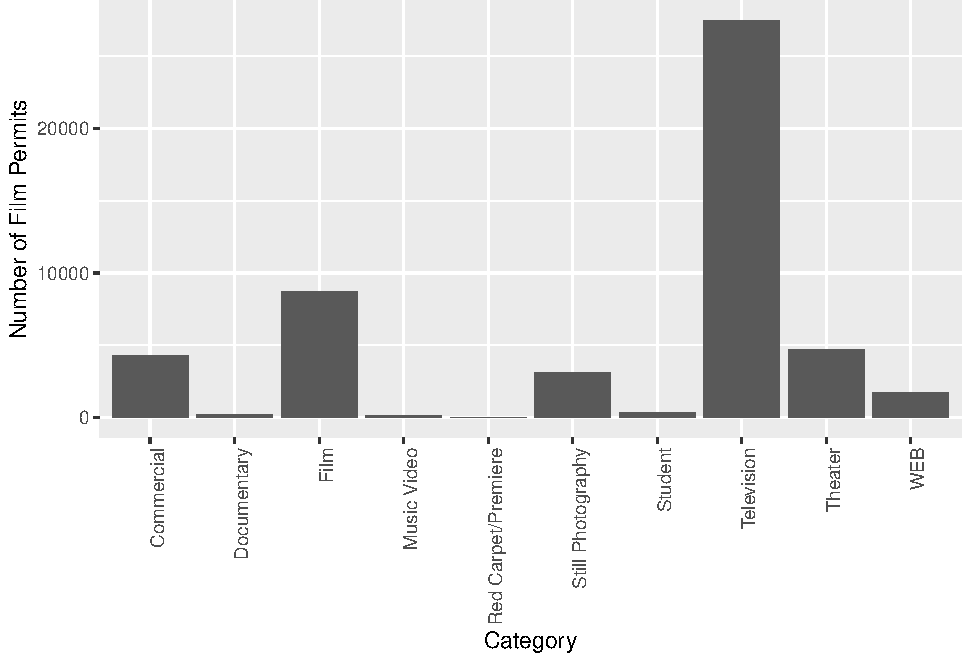
\includegraphics{Programming_Crump_files/figure-latex/unnamed-chunk-9-1.pdf}

\subsubsection{xlab() changes x label}\label{xlab-changes-x-label}

Let's slightly modify the x label too:

\begin{Shaded}
\begin{Highlighting}[]
\KeywordTok{ggplot}\NormalTok{(counts, }\KeywordTok{aes}\NormalTok{(}\DataTypeTok{x =} \NormalTok{Category, }\DataTypeTok{y =} \NormalTok{count_of_permits )) +}
\StringTok{  }\KeywordTok{geom_bar}\NormalTok{(}\DataTypeTok{stat=}\StringTok{"identity"}\NormalTok{) +}\StringTok{ }
\StringTok{  }\KeywordTok{theme}\NormalTok{(}\DataTypeTok{axis.text.x =} \KeywordTok{element_text}\NormalTok{(}\DataTypeTok{angle =} \DecValTok{90}\NormalTok{, }\DataTypeTok{hjust =} \DecValTok{1}\NormalTok{)) +}
\StringTok{  }\KeywordTok{ylab}\NormalTok{(}\StringTok{"Number of Film Permits"}\NormalTok{) +}\StringTok{ }
\StringTok{  }\KeywordTok{xlab}\NormalTok{(}\StringTok{"Category of film"}\NormalTok{)}
\end{Highlighting}
\end{Shaded}

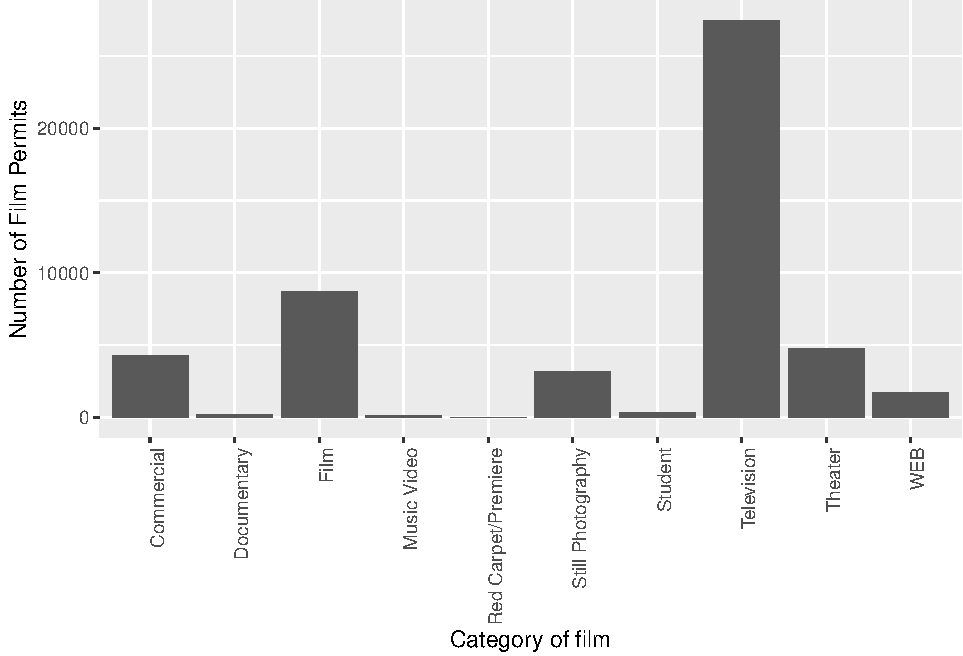
\includegraphics{Programming_Crump_files/figure-latex/unnamed-chunk-10-1.pdf}

\subsubsection{ggtitle() adds title}\label{ggtitle-adds-title}

Let's give our graph a title

\begin{Shaded}
\begin{Highlighting}[]
\KeywordTok{ggplot}\NormalTok{(counts, }\KeywordTok{aes}\NormalTok{(}\DataTypeTok{x =} \NormalTok{Category, }\DataTypeTok{y =} \NormalTok{count_of_permits )) +}
\StringTok{  }\KeywordTok{geom_bar}\NormalTok{(}\DataTypeTok{stat=}\StringTok{"identity"}\NormalTok{) +}\StringTok{ }
\StringTok{  }\KeywordTok{theme}\NormalTok{(}\DataTypeTok{axis.text.x =} \KeywordTok{element_text}\NormalTok{(}\DataTypeTok{angle =} \DecValTok{90}\NormalTok{, }\DataTypeTok{hjust =} \DecValTok{1}\NormalTok{)) +}
\StringTok{  }\KeywordTok{ylab}\NormalTok{(}\StringTok{"Number of Film Permits"}\NormalTok{) +}\StringTok{ }
\StringTok{  }\KeywordTok{xlab}\NormalTok{(}\StringTok{"Category of film"}\NormalTok{) +}
\StringTok{  }\KeywordTok{ggtitle}\NormalTok{(}\StringTok{"Number of Film permits in NYC by Category"}\NormalTok{)}
\end{Highlighting}
\end{Shaded}

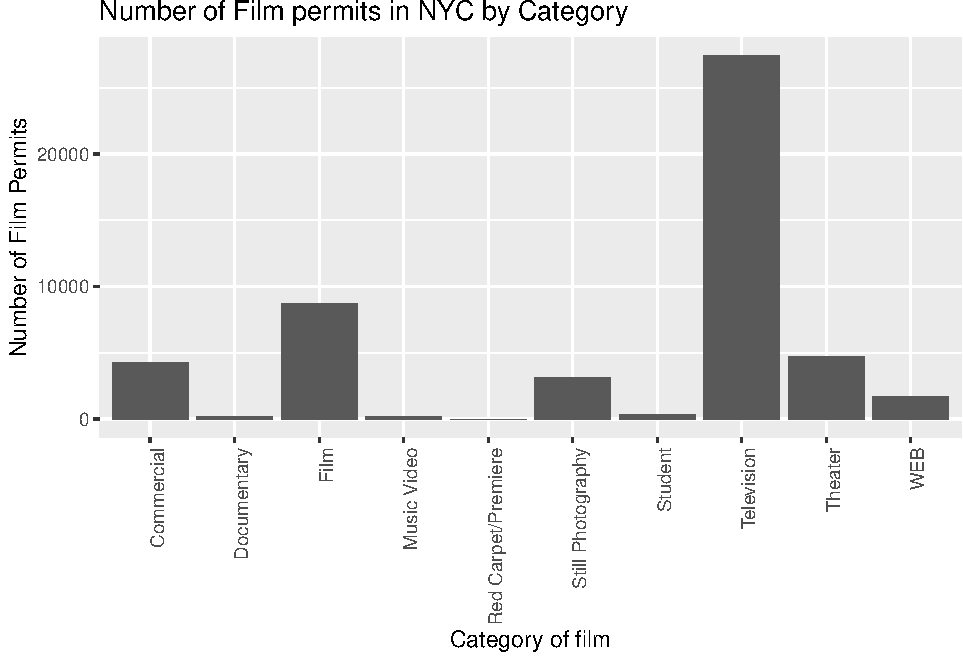
\includegraphics{Programming_Crump_files/figure-latex/unnamed-chunk-11-1.pdf}

\subsubsection{color adds color}\label{color-adds-color}

Let's make the bars different colors. To do this, we add new code to the
inside of the \texttt{aes()} part:

\begin{Shaded}
\begin{Highlighting}[]
\KeywordTok{ggplot}\NormalTok{(counts, }\KeywordTok{aes}\NormalTok{(}\DataTypeTok{x =} \NormalTok{Category, }\DataTypeTok{y =} \NormalTok{count_of_permits, }\DataTypeTok{color=}\NormalTok{Category )) +}
\StringTok{  }\KeywordTok{geom_bar}\NormalTok{(}\DataTypeTok{stat=}\StringTok{"identity"}\NormalTok{) +}\StringTok{ }
\StringTok{  }\KeywordTok{theme}\NormalTok{(}\DataTypeTok{axis.text.x =} \KeywordTok{element_text}\NormalTok{(}\DataTypeTok{angle =} \DecValTok{90}\NormalTok{, }\DataTypeTok{hjust =} \DecValTok{1}\NormalTok{)) +}
\StringTok{  }\KeywordTok{ylab}\NormalTok{(}\StringTok{"Number of Film Permits"}\NormalTok{) +}\StringTok{ }
\StringTok{  }\KeywordTok{xlab}\NormalTok{(}\StringTok{"Category of film"}\NormalTok{) +}
\StringTok{  }\KeywordTok{ggtitle}\NormalTok{(}\StringTok{"Number of Film permits in NYC by Category"}\NormalTok{)}
\end{Highlighting}
\end{Shaded}

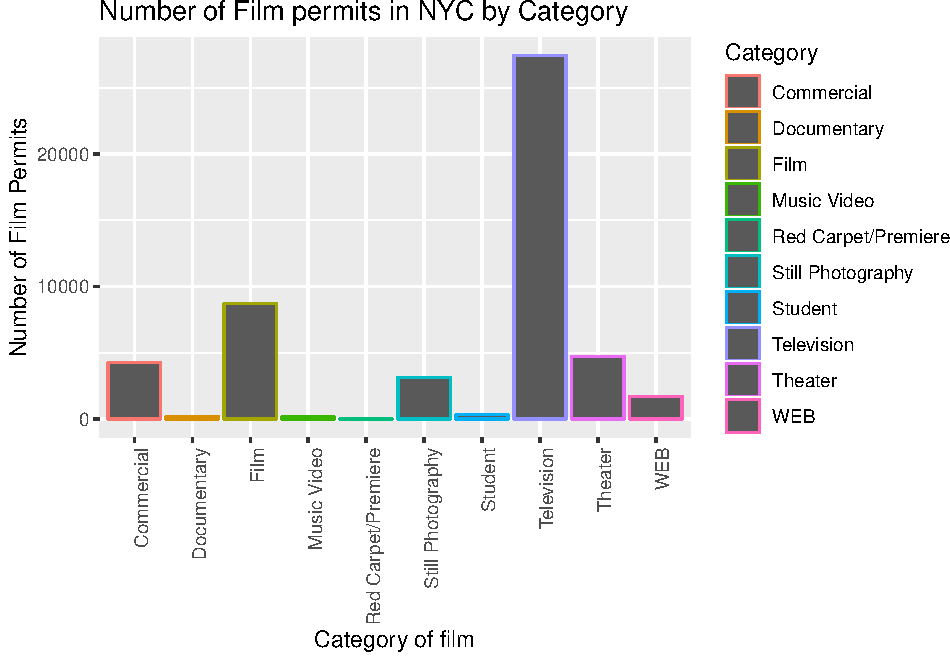
\includegraphics{Programming_Crump_files/figure-latex/unnamed-chunk-12-1.pdf}

\subsubsection{fill fills in color}\label{fill-fills-in-color}

Let's make the bars different colors. To do this, we add new code to the
inside of the \texttt{aes()} part\ldots{}Notice I've started using new
lines to make the code more readable.

\begin{Shaded}
\begin{Highlighting}[]
\KeywordTok{ggplot}\NormalTok{(counts, }\KeywordTok{aes}\NormalTok{(}\DataTypeTok{x =} \NormalTok{Category, }\DataTypeTok{y =} \NormalTok{count_of_permits, }
                   \DataTypeTok{color=}\NormalTok{Category, }
                   \DataTypeTok{fill=} \NormalTok{Category )) +}
\StringTok{  }\KeywordTok{geom_bar}\NormalTok{(}\DataTypeTok{stat=}\StringTok{"identity"}\NormalTok{) +}\StringTok{ }
\StringTok{  }\KeywordTok{theme}\NormalTok{(}\DataTypeTok{axis.text.x =} \KeywordTok{element_text}\NormalTok{(}\DataTypeTok{angle =} \DecValTok{90}\NormalTok{, }\DataTypeTok{hjust =} \DecValTok{1}\NormalTok{)) +}
\StringTok{  }\KeywordTok{ylab}\NormalTok{(}\StringTok{"Number of Film Permits"}\NormalTok{) +}\StringTok{ }
\StringTok{  }\KeywordTok{xlab}\NormalTok{(}\StringTok{"Category of film"}\NormalTok{) +}
\StringTok{  }\KeywordTok{ggtitle}\NormalTok{(}\StringTok{"Number of Film permits in NYC by Category"}\NormalTok{)}
\end{Highlighting}
\end{Shaded}

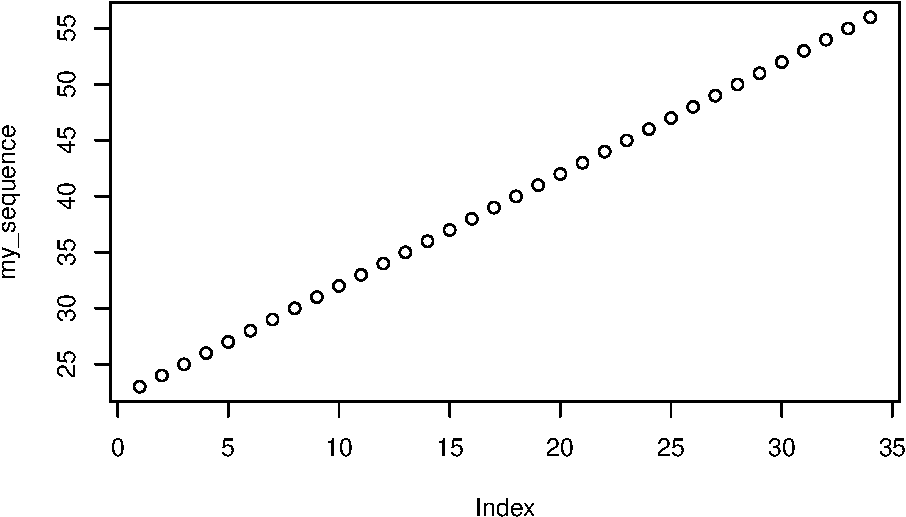
\includegraphics{Programming_Crump_files/figure-latex/unnamed-chunk-13-1.pdf}

\subsubsection{get rid of the legend}\label{get-rid-of-the-legend}

Sometimes you just don't want the legend on the side, to remove it add

\texttt{theme(legend.position="none")}

\begin{Shaded}
\begin{Highlighting}[]
\KeywordTok{ggplot}\NormalTok{(counts, }\KeywordTok{aes}\NormalTok{(}\DataTypeTok{x =} \NormalTok{Category, }\DataTypeTok{y =} \NormalTok{count_of_permits, }
                   \DataTypeTok{color=}\NormalTok{Category, }
                   \DataTypeTok{fill=} \NormalTok{Category )) +}
\StringTok{  }\KeywordTok{geom_bar}\NormalTok{(}\DataTypeTok{stat=}\StringTok{"identity"}\NormalTok{) +}\StringTok{ }
\StringTok{  }\KeywordTok{theme}\NormalTok{(}\DataTypeTok{axis.text.x =} \KeywordTok{element_text}\NormalTok{(}\DataTypeTok{angle =} \DecValTok{90}\NormalTok{, }\DataTypeTok{hjust =} \DecValTok{1}\NormalTok{)) +}
\StringTok{  }\KeywordTok{ylab}\NormalTok{(}\StringTok{"Number of Film Permits"}\NormalTok{) +}\StringTok{ }
\StringTok{  }\KeywordTok{xlab}\NormalTok{(}\StringTok{"Category of film"}\NormalTok{) +}
\StringTok{  }\KeywordTok{ggtitle}\NormalTok{(}\StringTok{"Number of Film permits in NYC by Category"}\NormalTok{) +}
\StringTok{  }\KeywordTok{theme}\NormalTok{(}\DataTypeTok{legend.position=}\StringTok{"none"}\NormalTok{)}
\end{Highlighting}
\end{Shaded}

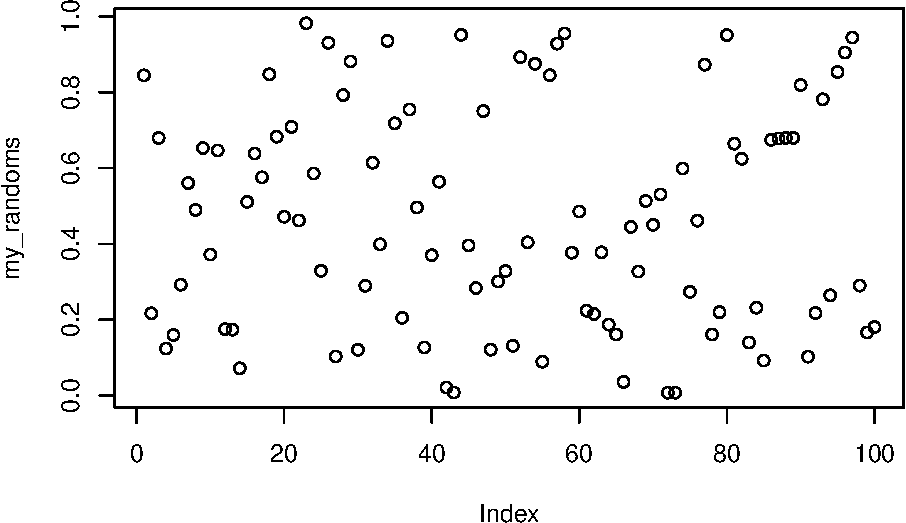
\includegraphics{Programming_Crump_files/figure-latex/unnamed-chunk-14-1.pdf}

\subsubsection{theme\_classic() makes white
background}\label{theme_classic-makes-white-background}

The rest is often just visual preference. For example, the graph above
has this grey grid behind the bars. For a clean classic no nonsense
look, use \texttt{theme\_classic()} to take away the grid.

\begin{Shaded}
\begin{Highlighting}[]
\KeywordTok{ggplot}\NormalTok{(counts, }\KeywordTok{aes}\NormalTok{(}\DataTypeTok{x =} \NormalTok{Category, }\DataTypeTok{y =} \NormalTok{count_of_permits, }
                   \DataTypeTok{color=}\NormalTok{Category, }
                   \DataTypeTok{fill=} \NormalTok{Category )) +}
\StringTok{  }\KeywordTok{geom_bar}\NormalTok{(}\DataTypeTok{stat=}\StringTok{"identity"}\NormalTok{) +}\StringTok{ }
\StringTok{  }\KeywordTok{theme}\NormalTok{(}\DataTypeTok{axis.text.x =} \KeywordTok{element_text}\NormalTok{(}\DataTypeTok{angle =} \DecValTok{90}\NormalTok{, }\DataTypeTok{hjust =} \DecValTok{1}\NormalTok{)) +}
\StringTok{  }\KeywordTok{ylab}\NormalTok{(}\StringTok{"Number of Film Permits"}\NormalTok{) +}\StringTok{ }
\StringTok{  }\KeywordTok{xlab}\NormalTok{(}\StringTok{"Category of film"}\NormalTok{) +}
\StringTok{  }\KeywordTok{ggtitle}\NormalTok{(}\StringTok{"Number of Film permits in NYC by Category"}\NormalTok{) +}
\StringTok{  }\KeywordTok{theme}\NormalTok{(}\DataTypeTok{legend.position=}\StringTok{"none"}\NormalTok{) +}
\StringTok{  }\KeywordTok{theme_classic}\NormalTok{()}
\end{Highlighting}
\end{Shaded}

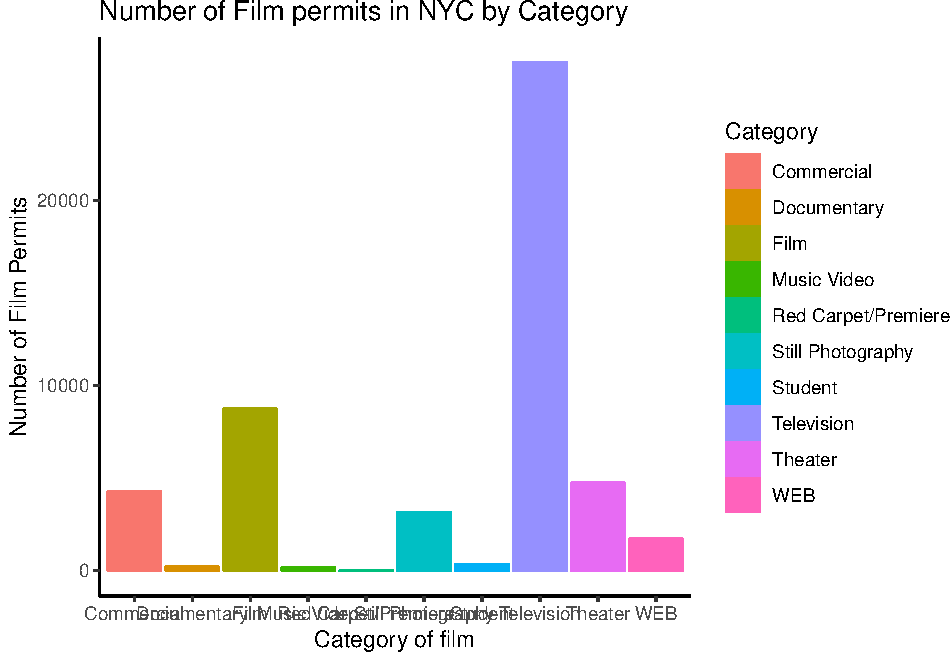
\includegraphics{Programming_Crump_files/figure-latex/unnamed-chunk-15-1.pdf}

\subsubsection{Sometimes layer order
matters}\label{sometimes-layer-order-matters}

Interesting, \texttt{theme\_classic()} is misbehaving a little bit. It
looks like we have some of our layer out of order, let's re-order. I
just moved \texttt{theme\_classic()} to just underneath the
\texttt{geom\_bar()} line. Now everything get's drawn properly.

\begin{Shaded}
\begin{Highlighting}[]
\KeywordTok{ggplot}\NormalTok{(counts, }\KeywordTok{aes}\NormalTok{(}\DataTypeTok{x =} \NormalTok{Category, }\DataTypeTok{y =} \NormalTok{count_of_permits, }
                   \DataTypeTok{color=}\NormalTok{Category, }
                   \DataTypeTok{fill=} \NormalTok{Category )) +}
\StringTok{  }\KeywordTok{geom_bar}\NormalTok{(}\DataTypeTok{stat=}\StringTok{"identity"}\NormalTok{) +}\StringTok{ }
\StringTok{  }\KeywordTok{theme_classic}\NormalTok{() +}
\StringTok{  }\KeywordTok{theme}\NormalTok{(}\DataTypeTok{axis.text.x =} \KeywordTok{element_text}\NormalTok{(}\DataTypeTok{angle =} \DecValTok{90}\NormalTok{, }\DataTypeTok{hjust =} \DecValTok{1}\NormalTok{)) +}
\StringTok{  }\KeywordTok{ylab}\NormalTok{(}\StringTok{"Number of Film Permits"}\NormalTok{) +}\StringTok{ }
\StringTok{  }\KeywordTok{xlab}\NormalTok{(}\StringTok{"Category of film"}\NormalTok{) +}
\StringTok{  }\KeywordTok{ggtitle}\NormalTok{(}\StringTok{"Number of Film permits in NYC by Category"}\NormalTok{) +}
\StringTok{  }\KeywordTok{theme}\NormalTok{(}\DataTypeTok{legend.position=}\StringTok{"none"}\NormalTok{) }
\end{Highlighting}
\end{Shaded}

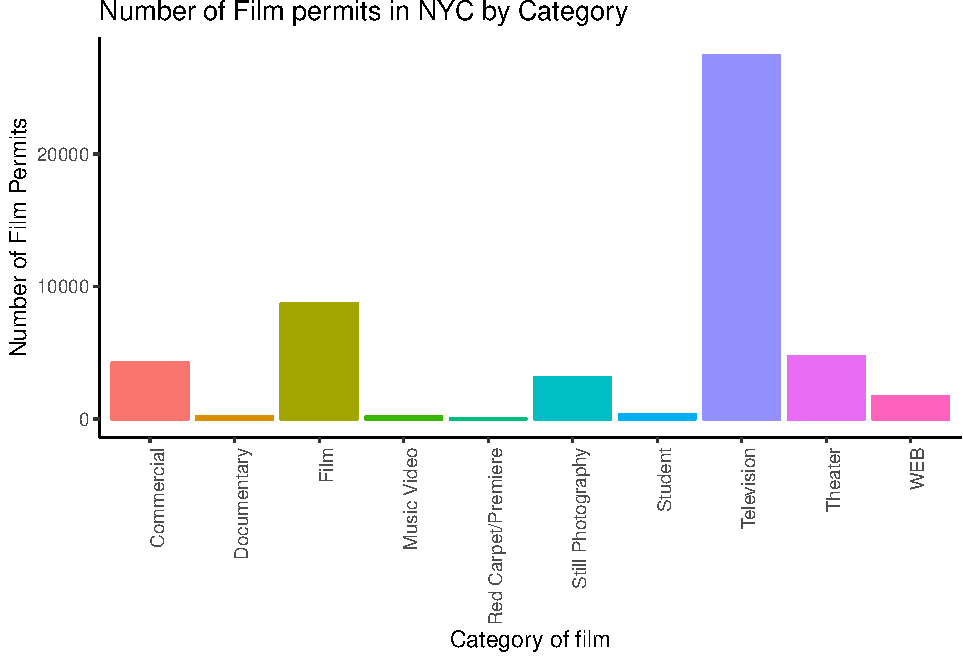
\includegraphics{Programming_Crump_files/figure-latex/unnamed-chunk-16-1.pdf}

\subsubsection{Font-size}\label{font-size}

Changing font-size is often something you want to do. ggplot2 can do
this in different ways. I suggest using the \texttt{base\_size} option
inside \texttt{theme\_classic()}. You set one number for the largest
font size in the graph, and everything else gets scaled to fit with that
that first number. It's really convenient. Look for the insisde of
\texttt{theme\_classic()}

\begin{Shaded}
\begin{Highlighting}[]
\KeywordTok{ggplot}\NormalTok{(counts, }\KeywordTok{aes}\NormalTok{(}\DataTypeTok{x =} \NormalTok{Category, }\DataTypeTok{y =} \NormalTok{count_of_permits, }
                   \DataTypeTok{color=}\NormalTok{Category, }
                   \DataTypeTok{fill=} \NormalTok{Category )) +}
\StringTok{  }\KeywordTok{geom_bar}\NormalTok{(}\DataTypeTok{stat=}\StringTok{"identity"}\NormalTok{) +}\StringTok{ }
\StringTok{  }\KeywordTok{theme_classic}\NormalTok{(}\DataTypeTok{base_size =} \DecValTok{15}\NormalTok{) +}
\StringTok{  }\KeywordTok{theme}\NormalTok{(}\DataTypeTok{axis.text.x =} \KeywordTok{element_text}\NormalTok{(}\DataTypeTok{angle =} \DecValTok{90}\NormalTok{, }\DataTypeTok{hjust =} \DecValTok{1}\NormalTok{)) +}
\StringTok{  }\KeywordTok{ylab}\NormalTok{(}\StringTok{"Number of Film Permits"}\NormalTok{) +}\StringTok{ }
\StringTok{  }\KeywordTok{xlab}\NormalTok{(}\StringTok{"Category of film"}\NormalTok{) +}
\StringTok{  }\KeywordTok{ggtitle}\NormalTok{(}\StringTok{"Number of Film permits in NYC by Category"}\NormalTok{) +}
\StringTok{  }\KeywordTok{theme}\NormalTok{(}\DataTypeTok{legend.position=}\StringTok{"none"}\NormalTok{) }
\end{Highlighting}
\end{Shaded}

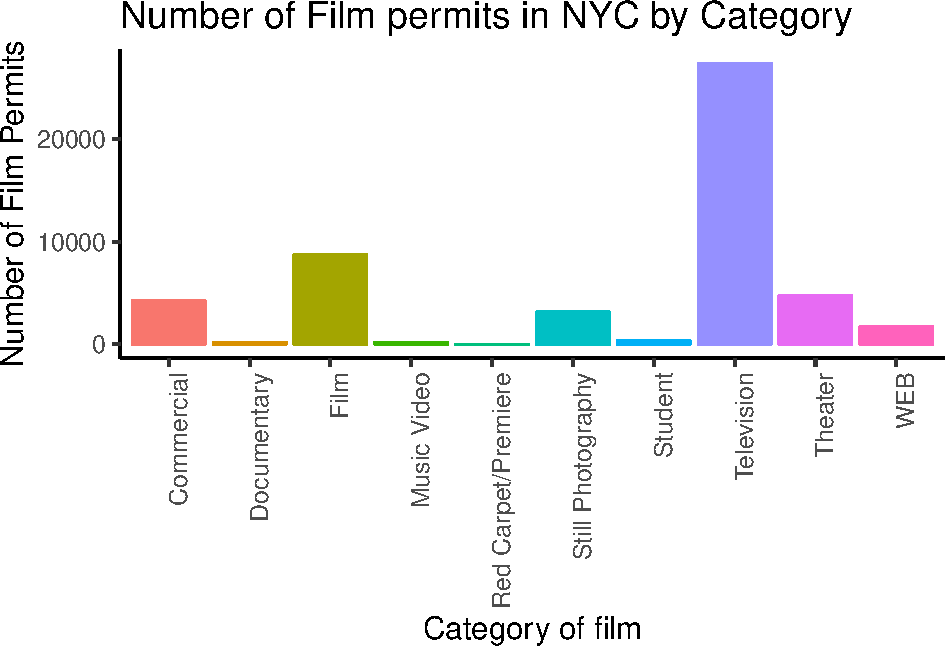
\includegraphics{Programming_Crump_files/figure-latex/unnamed-chunk-17-1.pdf}
or make things small\ldots{} just to see what happens

\begin{Shaded}
\begin{Highlighting}[]
\KeywordTok{ggplot}\NormalTok{(counts, }\KeywordTok{aes}\NormalTok{(}\DataTypeTok{x =} \NormalTok{Category, }\DataTypeTok{y =} \NormalTok{count_of_permits, }
                   \DataTypeTok{color=}\NormalTok{Category, }
                   \DataTypeTok{fill=} \NormalTok{Category )) +}
\StringTok{  }\KeywordTok{geom_bar}\NormalTok{(}\DataTypeTok{stat=}\StringTok{"identity"}\NormalTok{) +}\StringTok{ }
\StringTok{  }\KeywordTok{theme_classic}\NormalTok{(}\DataTypeTok{base_size =} \DecValTok{10}\NormalTok{) +}
\StringTok{  }\KeywordTok{theme}\NormalTok{(}\DataTypeTok{axis.text.x =} \KeywordTok{element_text}\NormalTok{(}\DataTypeTok{angle =} \DecValTok{90}\NormalTok{, }\DataTypeTok{hjust =} \DecValTok{1}\NormalTok{)) +}
\StringTok{  }\KeywordTok{ylab}\NormalTok{(}\StringTok{"Number of Film Permits"}\NormalTok{) +}\StringTok{ }
\StringTok{  }\KeywordTok{xlab}\NormalTok{(}\StringTok{"Category of film"}\NormalTok{) +}
\StringTok{  }\KeywordTok{ggtitle}\NormalTok{(}\StringTok{"Number of Film permits in NYC by Category"}\NormalTok{) +}
\StringTok{  }\KeywordTok{theme}\NormalTok{(}\DataTypeTok{legend.position=}\StringTok{"none"}\NormalTok{) }
\end{Highlighting}
\end{Shaded}

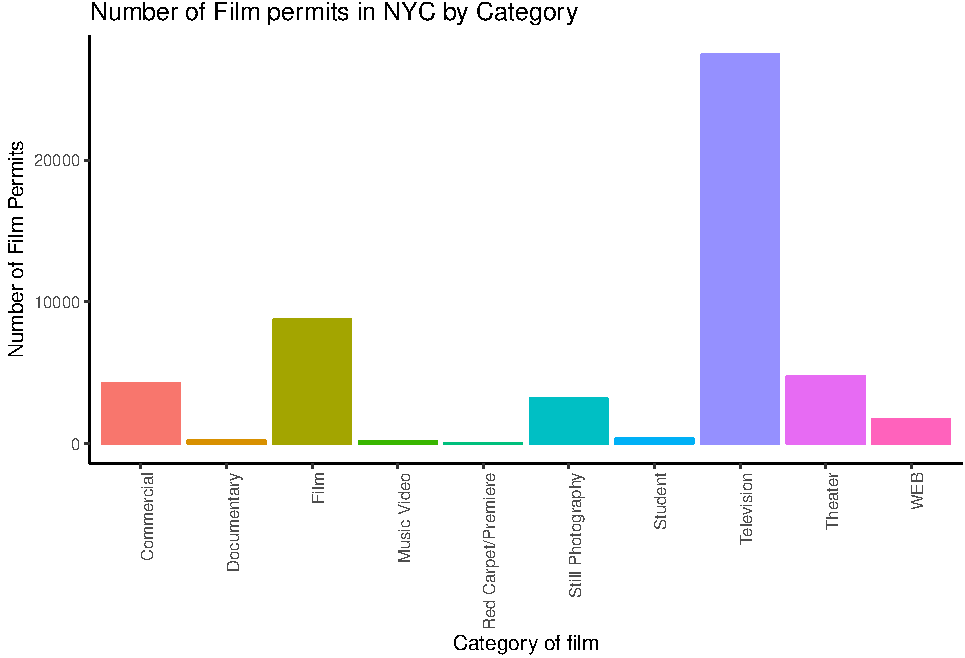
\includegraphics{Programming_Crump_files/figure-latex/unnamed-chunk-18-1.pdf}

\subsubsection{ggplot2 summary}\label{ggplot2-summary}

That's enough of the ggplot2 basics for now. You will discover that many
things are possible with ggplot2. It is amazing. We are going to get
back to answering some questions about the data with graphs. But, now
that we have built the code to make the graphs, all we need to do is
copy-paste, and make a few small changes, and boom, we have our graph.

\subsection{More questions about NYC
films}\label{more-questions-about-nyc-films}

\subsubsection{What are the sub-categories of
films?}\label{what-are-the-sub-categories-of-films}

Notice the \texttt{nyc\_films} data frame also has a column for
\texttt{SubCategoryName}. Let's see what's going on there with a quick
plot.

\begin{Shaded}
\begin{Highlighting}[]
\CommentTok{# get the counts (this is a comment it's just here for you to read)}

\NormalTok{counts <-}\StringTok{ }\NormalTok{nyc_films %>%}
\StringTok{          }\KeywordTok{group_by}\NormalTok{(SubCategoryName) %>%}
\StringTok{          }\KeywordTok{summarize}\NormalTok{(}\DataTypeTok{count_of_permits =} \KeywordTok{length}\NormalTok{(SubCategoryName))}

\CommentTok{# make the plot}

\KeywordTok{ggplot}\NormalTok{(counts, }\KeywordTok{aes}\NormalTok{(}\DataTypeTok{x =} \NormalTok{SubCategoryName, }\DataTypeTok{y =} \NormalTok{count_of_permits, }
                   \DataTypeTok{color=}\NormalTok{SubCategoryName, }
                   \DataTypeTok{fill=} \NormalTok{SubCategoryName )) +}
\StringTok{  }\KeywordTok{geom_bar}\NormalTok{(}\DataTypeTok{stat=}\StringTok{"identity"}\NormalTok{) +}\StringTok{ }
\StringTok{  }\KeywordTok{theme_classic}\NormalTok{(}\DataTypeTok{base_size =} \DecValTok{10}\NormalTok{) +}
\StringTok{  }\KeywordTok{theme}\NormalTok{(}\DataTypeTok{axis.text.x =} \KeywordTok{element_text}\NormalTok{(}\DataTypeTok{angle =} \DecValTok{90}\NormalTok{, }\DataTypeTok{hjust =} \DecValTok{1}\NormalTok{)) +}
\StringTok{  }\KeywordTok{ylab}\NormalTok{(}\StringTok{"Number of Film Permits"}\NormalTok{) +}\StringTok{ }
\StringTok{  }\KeywordTok{xlab}\NormalTok{(}\StringTok{"Sub-category of film"}\NormalTok{) +}
\StringTok{  }\KeywordTok{ggtitle}\NormalTok{(}\StringTok{"Number of Film permits in NYC by Sub-category"}\NormalTok{) +}
\StringTok{  }\KeywordTok{theme}\NormalTok{(}\DataTypeTok{legend.position=}\StringTok{"none"}\NormalTok{) }
\end{Highlighting}
\end{Shaded}

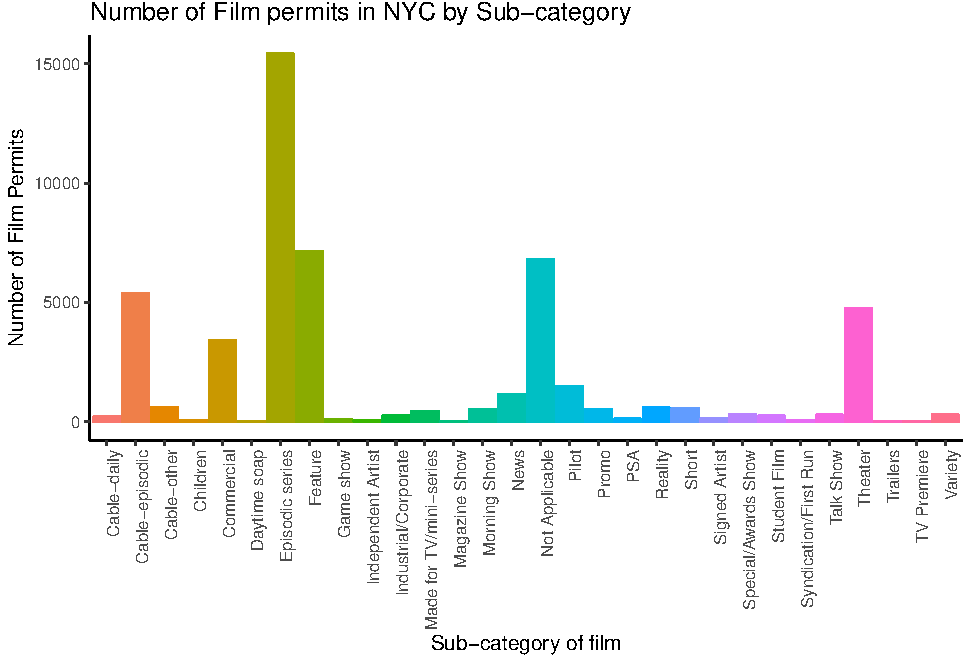
\includegraphics{Programming_Crump_files/figure-latex/unnamed-chunk-19-1.pdf}

I guess ``episodic series'' are the most common. Using a graph like this
gave us our answer super fast.

\subsubsection{Categories by different
Boroughs}\label{categories-by-different-boroughs}

Let's see one more really useful thing about ggplot2. It's called
\texttt{facet\_wrap()}. It's an ugly word, but you will see that it is
very cool, and you can do next-level-super-hero graph styles with
\texttt{facet\_wrap} that other people can't do very easily.

Here's our question. We know that some films are made in different
Boroughs, and that sme films are made in different categories, but do
different Boroughs have different patterns for the kinds of categories
of films they request permits for? Are their more tv shows in Brookyln?
How do we find out? Watch, just like this:

\begin{Shaded}
\begin{Highlighting}[]
\CommentTok{# get the counts (this is a comment it's just here for you to read)}

\NormalTok{counts <-}\StringTok{ }\NormalTok{nyc_films %>%}
\StringTok{          }\KeywordTok{group_by}\NormalTok{(Borough,Category) %>%}
\StringTok{          }\KeywordTok{summarize}\NormalTok{(}\DataTypeTok{count_of_permits =} \KeywordTok{length}\NormalTok{(Category))}

\CommentTok{# make the plot}

\KeywordTok{ggplot}\NormalTok{(counts, }\KeywordTok{aes}\NormalTok{(}\DataTypeTok{x =} \NormalTok{Category, }\DataTypeTok{y =} \NormalTok{count_of_permits, }
                   \DataTypeTok{color=}\NormalTok{Category, }
                   \DataTypeTok{fill=} \NormalTok{Category )) +}
\StringTok{  }\KeywordTok{geom_bar}\NormalTok{(}\DataTypeTok{stat=}\StringTok{"identity"}\NormalTok{) +}\StringTok{ }
\StringTok{  }\KeywordTok{theme_classic}\NormalTok{(}\DataTypeTok{base_size =} \DecValTok{10}\NormalTok{) +}
\StringTok{  }\KeywordTok{theme}\NormalTok{(}\DataTypeTok{axis.text.x =} \KeywordTok{element_text}\NormalTok{(}\DataTypeTok{angle =} \DecValTok{90}\NormalTok{, }\DataTypeTok{hjust =} \DecValTok{1}\NormalTok{)) +}
\StringTok{  }\KeywordTok{ylab}\NormalTok{(}\StringTok{"Number of Film Permits"}\NormalTok{) +}\StringTok{ }
\StringTok{  }\KeywordTok{xlab}\NormalTok{(}\StringTok{"Category of film"}\NormalTok{) +}
\StringTok{  }\KeywordTok{ggtitle}\NormalTok{(}\StringTok{"Number of Film permits in NYC by Category and Borough"}\NormalTok{) +}
\StringTok{  }\KeywordTok{theme}\NormalTok{(}\DataTypeTok{legend.position=}\StringTok{"none"}\NormalTok{) +}
\StringTok{  }\KeywordTok{facet_wrap}\NormalTok{(~Borough, }\DataTypeTok{ncol=}\DecValTok{3}\NormalTok{)}
\end{Highlighting}
\end{Shaded}

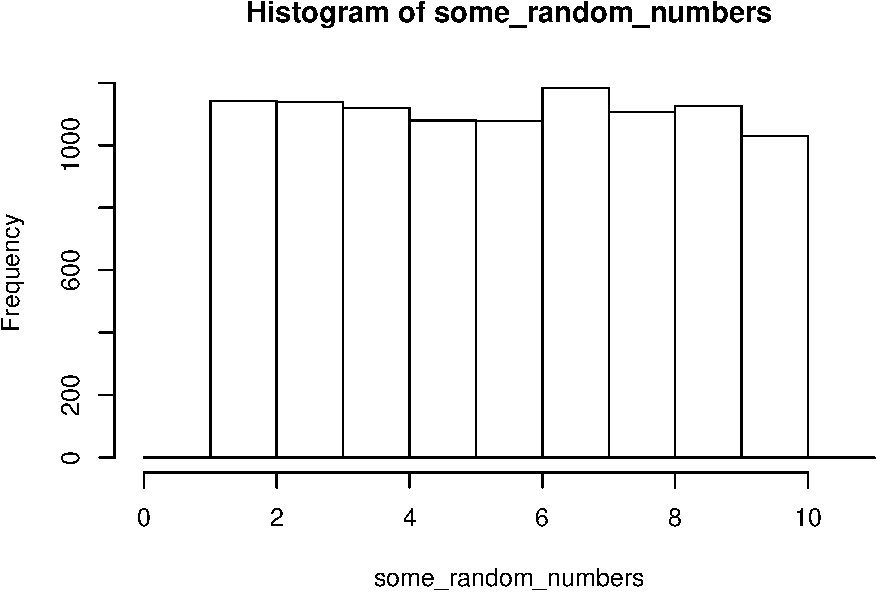
\includegraphics{Programming_Crump_files/figure-latex/unnamed-chunk-20-1.pdf}

We did two important things. First we added \texttt{Borough} and
\texttt{Category} into the \texttt{group\_by()} function. This
automatically gives separate counts for each category of film, for each
Borough. Then we added
\texttt{facet\_wrap(\textasciitilde{}Borough,\ ncol=3)} to the end of
the plot, and it automatically drew us 5 different bar graphs, one for
each Borough! That was fast. Imagine doing that by hand.

The nice thing about this is we can switch things around if we want. For
example, we could do it this way by switching the \texttt{Category} with
\texttt{Borough}, and facet-wrapping by Category instead of Borough like
we did above. Do what works for you.

\begin{Shaded}
\begin{Highlighting}[]
\KeywordTok{ggplot}\NormalTok{(counts, }\KeywordTok{aes}\NormalTok{(}\DataTypeTok{x =} \NormalTok{Borough, }\DataTypeTok{y =} \NormalTok{count_of_permits, }
                   \DataTypeTok{color=}\NormalTok{Borough, }
                   \DataTypeTok{fill=} \NormalTok{Borough )) +}
\StringTok{  }\KeywordTok{geom_bar}\NormalTok{(}\DataTypeTok{stat=}\StringTok{"identity"}\NormalTok{) +}\StringTok{ }
\StringTok{  }\KeywordTok{theme_classic}\NormalTok{(}\DataTypeTok{base_size =} \DecValTok{10}\NormalTok{) +}
\StringTok{  }\KeywordTok{theme}\NormalTok{(}\DataTypeTok{axis.text.x =} \KeywordTok{element_text}\NormalTok{(}\DataTypeTok{angle =} \DecValTok{90}\NormalTok{, }\DataTypeTok{hjust =} \DecValTok{1}\NormalTok{)) +}
\StringTok{  }\KeywordTok{ylab}\NormalTok{(}\StringTok{"Number of Film Permits"}\NormalTok{) +}\StringTok{ }
\StringTok{  }\KeywordTok{xlab}\NormalTok{(}\StringTok{"Borough"}\NormalTok{) +}
\StringTok{  }\KeywordTok{ggtitle}\NormalTok{(}\StringTok{"Number of Film permits in NYC by Category and Borough"}\NormalTok{) +}
\StringTok{  }\KeywordTok{theme}\NormalTok{(}\DataTypeTok{legend.position=}\StringTok{"none"}\NormalTok{) +}
\StringTok{  }\KeywordTok{facet_wrap}\NormalTok{(~Category, }\DataTypeTok{ncol=}\DecValTok{5}\NormalTok{)}
\end{Highlighting}
\end{Shaded}

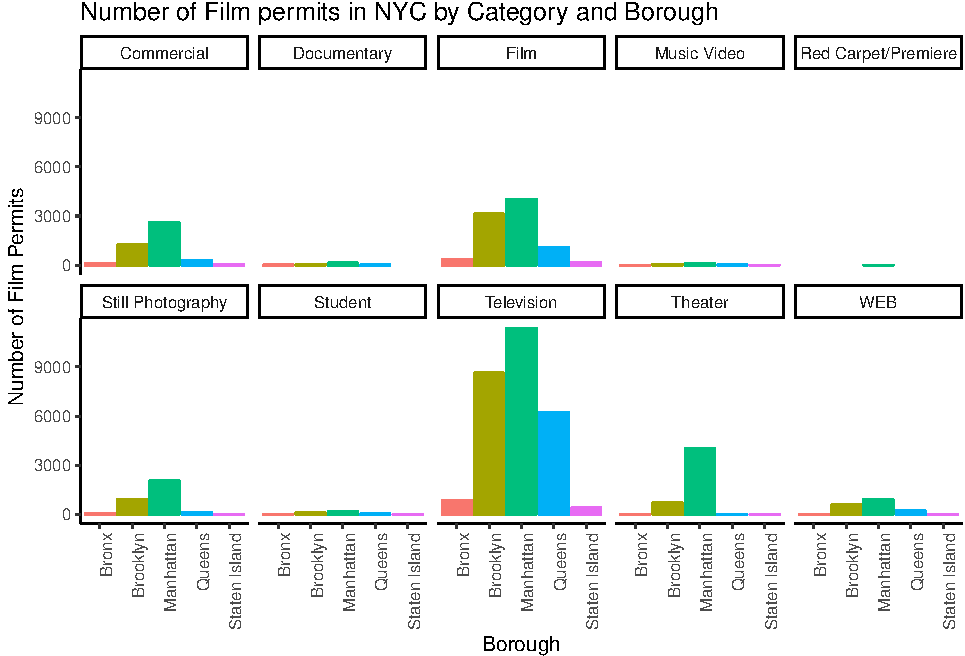
\includegraphics{Programming_Crump_files/figure-latex/unnamed-chunk-21-1.pdf}

\subsection{Gapminder Data}\label{gapminder-data}

\url{https://www.gapminder.org} is an organization that collects some
really interesting worldwide data. They also make cool visualization
tools for looking at the data. There are many neat examples, and they
have visualization tools built right into their website that you can
play around with \url{https://www.gapminder.org/tools/}. That's fun
check it out.

There is also an R package called \texttt{gapminder}. When you install
this package, it loads in some of the data from gapminder, so we can
play with it in R.

If you don't have the gapminder packe installed, you can install it by
running this code

\begin{Shaded}
\begin{Highlighting}[]
\KeywordTok{install.packages}\NormalTok{(}\StringTok{"gapminder"}\NormalTok{)}
\end{Highlighting}
\end{Shaded}

Once the package is installed, you need to load the new library, like
this. Then, you can put the \texttt{gapminder} data into a data frame,
like we do here: \texttt{gapminder\_df}.

\begin{Shaded}
\begin{Highlighting}[]
\KeywordTok{library}\NormalTok{(gapminder)}
\NormalTok{gapminder_df<-gapminder}
\end{Highlighting}
\end{Shaded}

\subsubsection{Look at the data frame}\label{look-at-the-data-frame}

You can look at the data frame to see what is in it, and you can use
\texttt{summarytools} again to view a summary of the data.

\begin{Shaded}
\begin{Highlighting}[]
\KeywordTok{view}\NormalTok{(}\KeywordTok{dfSummary}\NormalTok{(gapminder_df))}
\end{Highlighting}
\end{Shaded}

There are 1704 rows of data, and we see some columns for country,
continent, year, life expectancy, population, and GDP per capita.

\subsection{Asking Questions with the gap minder
data}\label{asking-questions-with-the-gap-minder-data}

We will show you how to graph some the data to answer a few different
kinds of questions. Then you will form your own questions, and see if
you can answer them with ggplot2 yourself. All you will need to do is
copy and paste the following examples, and change them up a little bit

\subsubsection{Life Expectancy
histogram}\label{life-expectancy-histogram}

How long are people living all around the world according to this data
set? There are many ways we could plot the data to find out. The first
way is a histogram. We have many numbers for life expectancy in the
column \texttt{lifeExp}. This is a big sample, full of numbers for 142
countries across many years. It's easy to make a histrogram in ggplot to
view the distribution:

\begin{Shaded}
\begin{Highlighting}[]
\KeywordTok{ggplot}\NormalTok{(gapminder_df, }\KeywordTok{aes}\NormalTok{(}\DataTypeTok{x=}\NormalTok{lifeExp))+}
\StringTok{  }\KeywordTok{geom_histogram}\NormalTok{(}\DataTypeTok{color=}\StringTok{"white"}\NormalTok{)}
\end{Highlighting}
\end{Shaded}

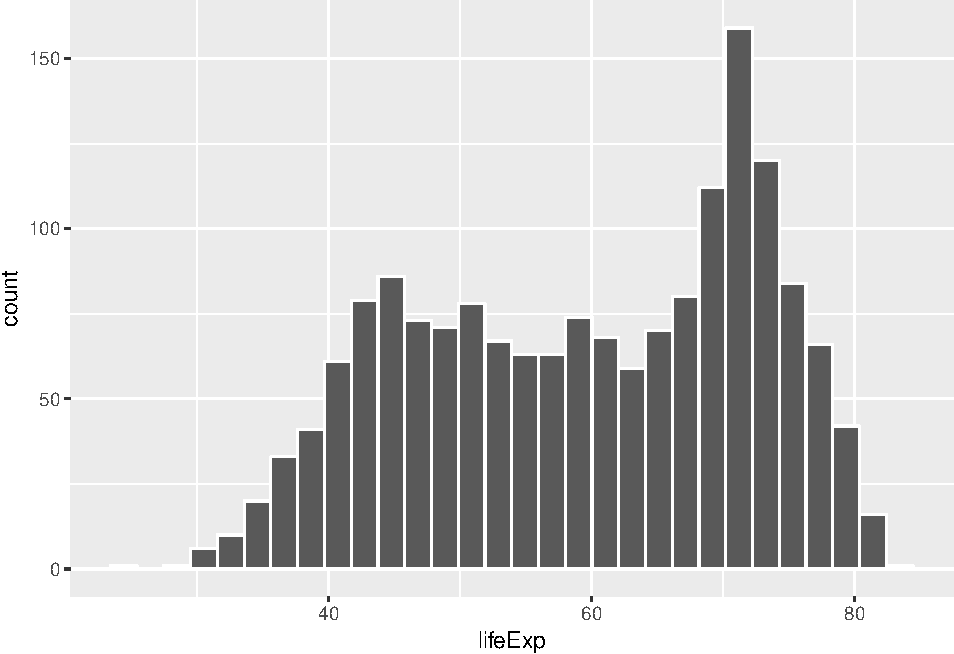
\includegraphics{Programming_Crump_files/figure-latex/unnamed-chunk-25-1.pdf}

See, that was easy. Next, is a code block that adds more layers and
settings if you wanted to modify parts of the graph:

\begin{Shaded}
\begin{Highlighting}[]
\KeywordTok{ggplot}\NormalTok{(gapminder_df, }\KeywordTok{aes}\NormalTok{(}\DataTypeTok{x =} \NormalTok{lifeExp)) +}
\StringTok{  }\KeywordTok{geom_histogram}\NormalTok{(}\DataTypeTok{color=}\StringTok{"white"}\NormalTok{)+}\StringTok{ }
\StringTok{  }\KeywordTok{theme_classic}\NormalTok{(}\DataTypeTok{base_size =} \DecValTok{15}\NormalTok{) +}
\StringTok{  }\KeywordTok{ylab}\NormalTok{(}\StringTok{"Frequency count"}\NormalTok{) +}\StringTok{ }
\StringTok{  }\KeywordTok{xlab}\NormalTok{(}\StringTok{"Life Expectancy"}\NormalTok{) +}
\StringTok{  }\KeywordTok{ggtitle}\NormalTok{(}\StringTok{"Histogram of Life Expectancy from Gapminder"}\NormalTok{)}
\end{Highlighting}
\end{Shaded}

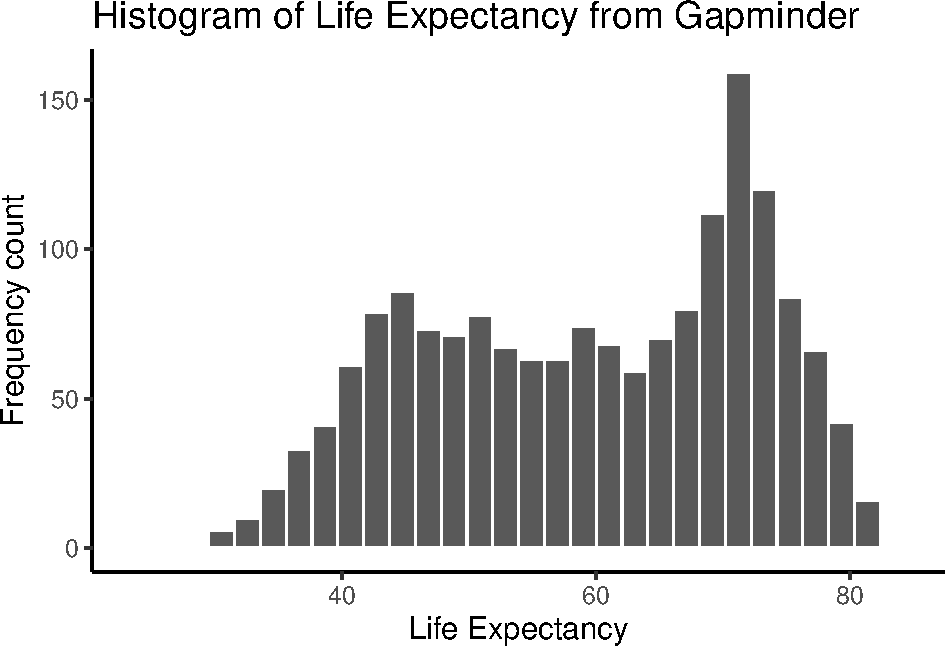
\includegraphics{Programming_Crump_files/figure-latex/unnamed-chunk-26-1.pdf}

The histogram shows a wide range of life expectancies, from below 40 to
just over 80. Histograms are useful, they can show you what kinds of
values happen more often than others.

One final thing about histograms in ggplot. You may want to change the
bin size. That controls how wide or narrow, or the number of bars (how
they split across the range), in the histogram. You need to set the
\texttt{bins=} option in \texttt{geom\_histogram()}.

\begin{Shaded}
\begin{Highlighting}[]
\KeywordTok{ggplot}\NormalTok{(gapminder_df, }\KeywordTok{aes}\NormalTok{(}\DataTypeTok{x =} \NormalTok{lifeExp)) +}
\StringTok{  }\KeywordTok{geom_histogram}\NormalTok{(}\DataTypeTok{color=}\StringTok{"white"}\NormalTok{, }\DataTypeTok{bins=}\DecValTok{50}\NormalTok{)+}\StringTok{ }
\StringTok{  }\KeywordTok{theme_classic}\NormalTok{(}\DataTypeTok{base_size =} \DecValTok{15}\NormalTok{) +}
\StringTok{  }\KeywordTok{ylab}\NormalTok{(}\StringTok{"Frequency count"}\NormalTok{) +}\StringTok{ }
\StringTok{  }\KeywordTok{xlab}\NormalTok{(}\StringTok{"Life Expectancy"}\NormalTok{) +}
\StringTok{  }\KeywordTok{ggtitle}\NormalTok{(}\StringTok{"Histogram of Life Expectancy from Gapminder"}\NormalTok{)}
\end{Highlighting}
\end{Shaded}

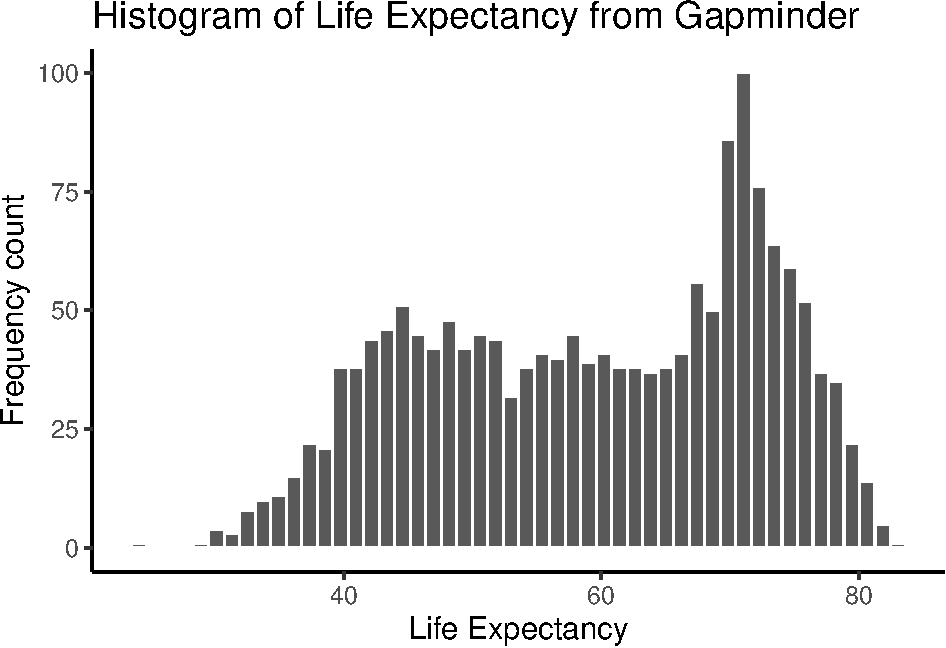
\includegraphics{Programming_Crump_files/figure-latex/unnamed-chunk-27-1.pdf}

See, same basic patter, but now breaking up the range into 50 little
equal sized bins, rather than 30, which is the default. You get to
choose what you want to do.

\subsubsection{Life Expectancy by year
Scatterplot}\label{life-expectancy-by-year-scatterplot}

We can see we have data for life expectancy and different years. So,
does worldwide life expectancy change across the years in the data set?
As we go into the future, are people living longer?

Let's look at this using a scatterplot. We can set the x-axis to be
year, and the y-axis to be life expectancy. Then we can use
\texttt{geom\_point()} to display a whole bunch of dots, and then look
at them. Here's the simple code:

\begin{Shaded}
\begin{Highlighting}[]
\KeywordTok{ggplot}\NormalTok{(gapminder_df, }\KeywordTok{aes}\NormalTok{(}\DataTypeTok{y=} \NormalTok{lifeExp, }\DataTypeTok{x=} \NormalTok{year))+}
\StringTok{  }\KeywordTok{geom_point}\NormalTok{()}
\end{Highlighting}
\end{Shaded}

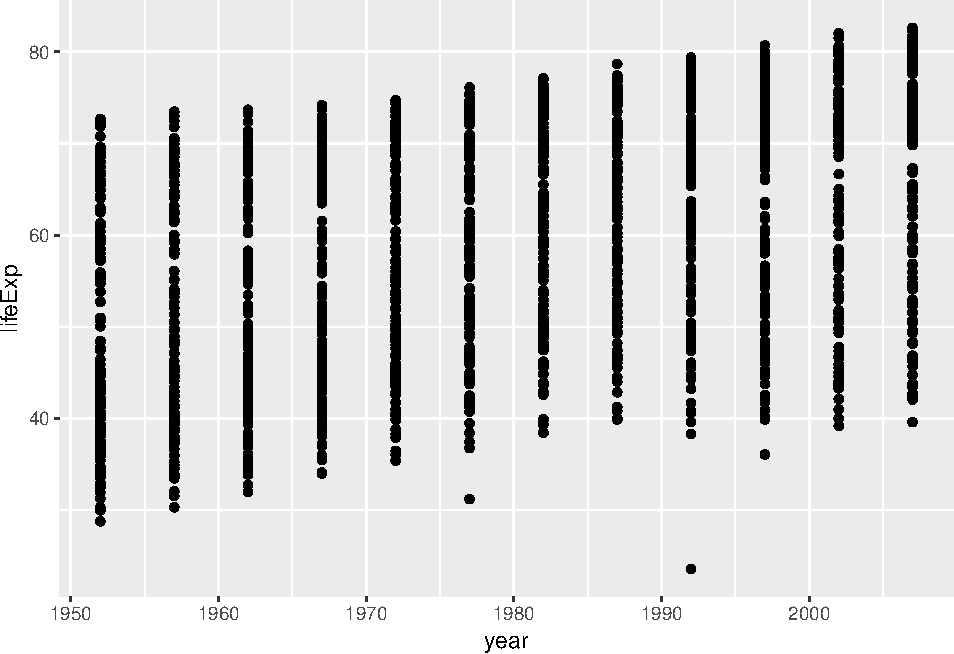
\includegraphics{Programming_Crump_files/figure-latex/unnamed-chunk-28-1.pdf}

Whoa, that's a lot of dots! Remember that each country is measured each
year. So, the bands of dots you see, show the life expectancies for the
whole range of countries within each year of the database. There is a
big spread inside each year. But, on the whole it looks like groups of
dots slowly go up over years.

\subsubsection{One country, life expectancy by
year}\label{one-country-life-expectancy-by-year}

I'm (Matt) from Canada, so maybe I want to know if life expectancy for
Canadians is going up over the years. To find out the answer for one
country, we first need to split the full data set, into another smaller
data set that only contains data for Canada. In other words, we want
only the rows where the word ``Canada'' is found in the \texttt{country}
column. We will use the \texttt{filter} function from `dplyr for this:

\begin{Shaded}
\begin{Highlighting}[]
\CommentTok{# filter rows to contain Canada}

\NormalTok{smaller_df <-}\StringTok{ }\NormalTok{gapminder_df %>%}\StringTok{ }
\StringTok{                 }\KeywordTok{filter}\NormalTok{(country ==}\StringTok{ "Canada"}\NormalTok{)}

\CommentTok{# plot the new data contained in smaller_df}

\KeywordTok{ggplot}\NormalTok{(smaller_df, }\KeywordTok{aes}\NormalTok{(}\DataTypeTok{y=} \NormalTok{lifeExp, }\DataTypeTok{x=} \NormalTok{year))+}
\StringTok{  }\KeywordTok{geom_point}\NormalTok{()}
\end{Highlighting}
\end{Shaded}

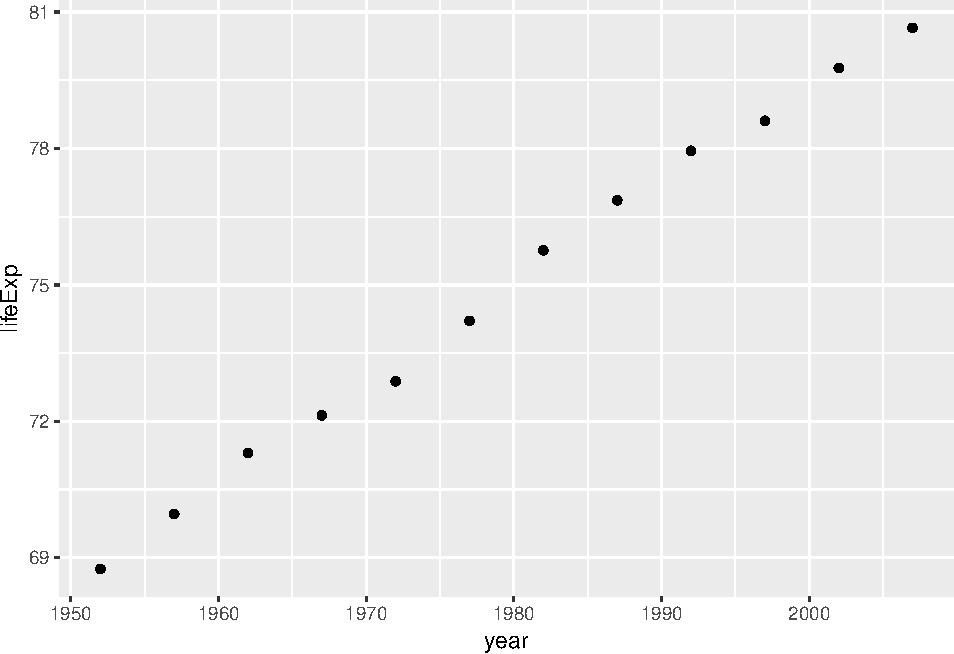
\includegraphics{Programming_Crump_files/figure-latex/unnamed-chunk-29-1.pdf}

I would say things are looking good for Canadians, their life expectancy
is going up over the years!

\subsubsection{Multiple countries
scatterplot}\label{multiple-countries-scatterplot}

What if we want to look at a few countries altogether. We can do this
too. We just change how we filter the data so more than one country is
allowed, then we plot the data. We will also add some nicer color
options and make the plot look pretty. First, the simple code:

\begin{Shaded}
\begin{Highlighting}[]
\CommentTok{# filter rows to contain countries of choice}

\NormalTok{smaller_df <-}\StringTok{ }\NormalTok{gapminder_df %>%}\StringTok{ }
\StringTok{                 }\KeywordTok{filter}\NormalTok{(country %in%}\StringTok{ }\KeywordTok{c}\NormalTok{(}\StringTok{"Canada"}\NormalTok{,}\StringTok{"France"}\NormalTok{,}\StringTok{"Brazil"}\NormalTok{) ==}\StringTok{ }\OtherTok{TRUE}\NormalTok{)}

\CommentTok{# plot the new data contained in smaller_df}

\KeywordTok{ggplot}\NormalTok{(smaller_df, }\KeywordTok{aes}\NormalTok{(}\DataTypeTok{y=} \NormalTok{lifeExp, }\DataTypeTok{x=} \NormalTok{year, }\DataTypeTok{group=} \NormalTok{country))+}
\StringTok{  }\KeywordTok{geom_point}\NormalTok{()}
\end{Highlighting}
\end{Shaded}

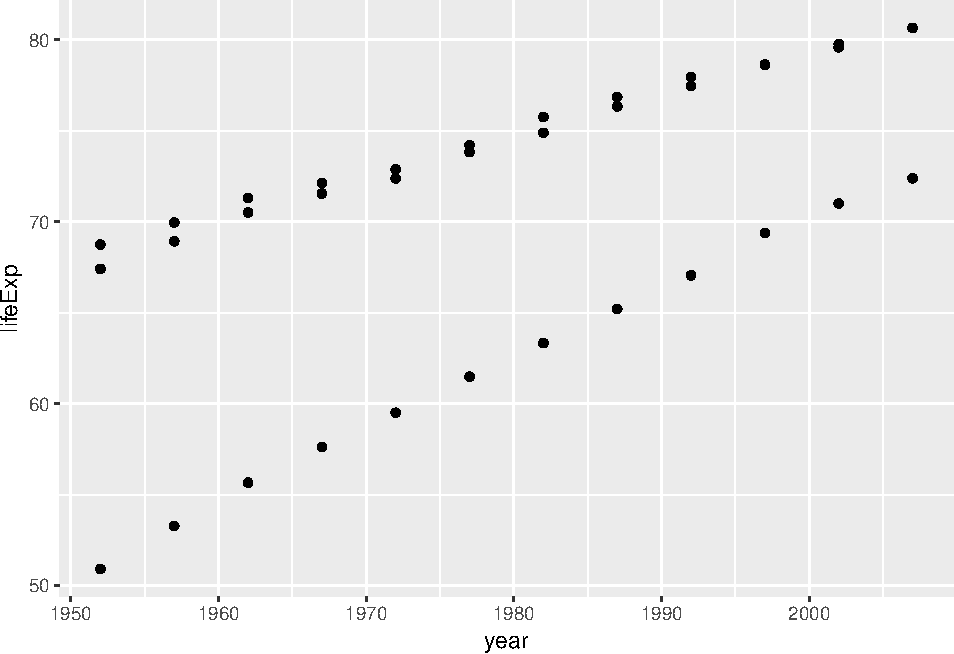
\includegraphics{Programming_Crump_files/figure-latex/unnamed-chunk-30-1.pdf}

Nice, we can now see three sets of dots, but which are countries do they
represent? Let's add a lengend, and make the graph better looking.

\begin{Shaded}
\begin{Highlighting}[]
\KeywordTok{ggplot}\NormalTok{(smaller_df,}\KeywordTok{aes}\NormalTok{(}\DataTypeTok{y=} \NormalTok{lifeExp, }\DataTypeTok{x=} \NormalTok{year, }
                      \DataTypeTok{group=} \NormalTok{country, }\DataTypeTok{color =} \NormalTok{country)) +}
\StringTok{  }\KeywordTok{geom_point}\NormalTok{()+}\StringTok{ }
\StringTok{  }\KeywordTok{theme_classic}\NormalTok{(}\DataTypeTok{base_size =} \DecValTok{15}\NormalTok{) +}
\StringTok{  }\KeywordTok{ylab}\NormalTok{(}\StringTok{"Life Expectancy"}\NormalTok{) +}\StringTok{ }
\StringTok{  }\KeywordTok{xlab}\NormalTok{(}\StringTok{"Year"}\NormalTok{) +}
\StringTok{  }\KeywordTok{ggtitle}\NormalTok{(}\StringTok{"Life expectancy by year for three countries"}\NormalTok{)}
\end{Highlighting}
\end{Shaded}

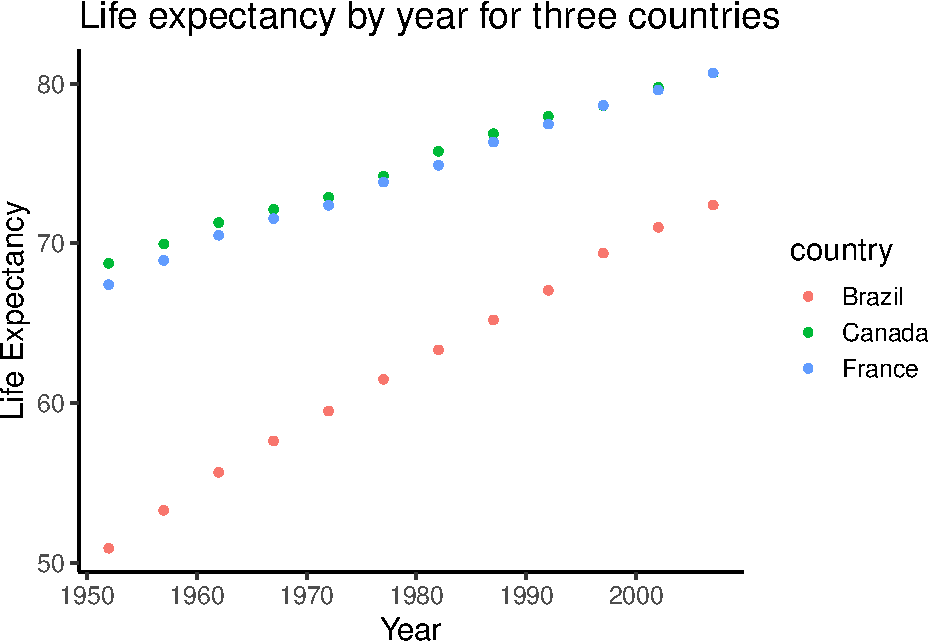
\includegraphics{Programming_Crump_files/figure-latex/unnamed-chunk-31-1.pdf}

\subsubsection{geom\_line() connecting the
dots}\label{geom_line-connecting-the-dots}

We might also want to connect the dots with a line, to make it easier to
see the connection! Remember, ggplot2 draws layers on top of layers. So,
we add in a new \texttt{geom\_line()} layer.

\begin{Shaded}
\begin{Highlighting}[]
\KeywordTok{ggplot}\NormalTok{(smaller_df,}\KeywordTok{aes}\NormalTok{(}\DataTypeTok{y=} \NormalTok{lifeExp, }\DataTypeTok{x=} \NormalTok{year, }
                      \DataTypeTok{group=} \NormalTok{country, }\DataTypeTok{color =} \NormalTok{country)) +}
\StringTok{  }\KeywordTok{geom_point}\NormalTok{()+}\StringTok{ }
\StringTok{  }\KeywordTok{geom_line}\NormalTok{()+}
\StringTok{  }\KeywordTok{theme_classic}\NormalTok{(}\DataTypeTok{base_size =} \DecValTok{15}\NormalTok{) +}
\StringTok{  }\KeywordTok{ylab}\NormalTok{(}\StringTok{"Life Expectancy"}\NormalTok{) +}\StringTok{ }
\StringTok{  }\KeywordTok{xlab}\NormalTok{(}\StringTok{"Year"}\NormalTok{) +}
\StringTok{  }\KeywordTok{ggtitle}\NormalTok{(}\StringTok{"Life expectancy by year for three countries"}\NormalTok{)}
\end{Highlighting}
\end{Shaded}

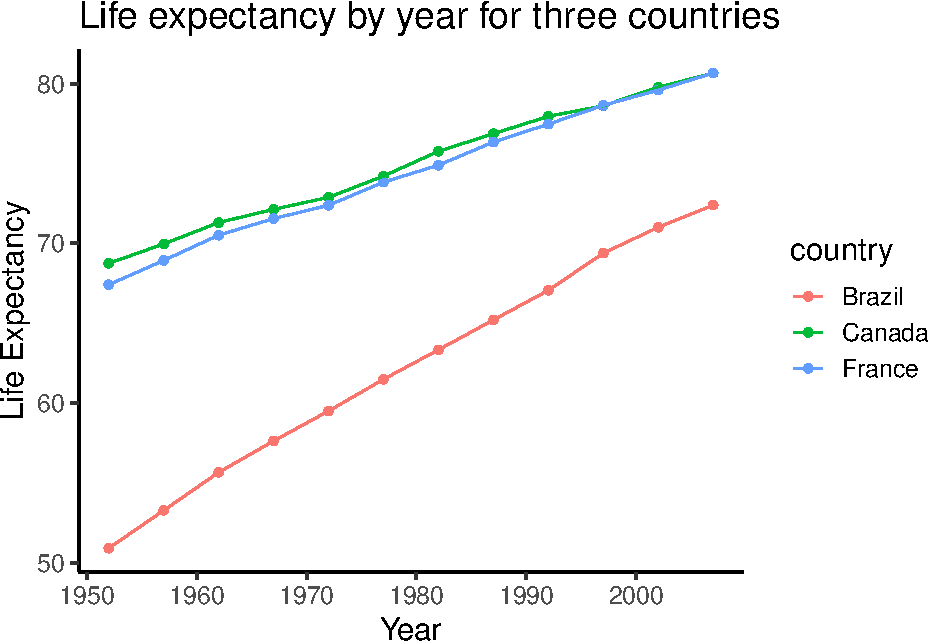
\includegraphics{Programming_Crump_files/figure-latex/unnamed-chunk-32-1.pdf}

Whenever you have a variable with multiple numbers, you can always plot
it, just like in the above example. Remember the variable
\emph{my\_numbers} contains 100 numbers. This means there are 100 slots
in the variable. Each slot has an \emph{index} value. The index value
for the first slot is 1, the index value for the second slot is 2, and
so on. The x-axis (the bottom line in the graph) shows the index value
from 1 to 100. Remember also, that each slot contains the number 43. The
y-axis (the vertical line in the graph) shows a range of numbers. The
dots in the graph represent the value inside each slot of the variable.
Because each slot contains the value 43, we see all 100 dots, all in a
line, all positioned at 43 with respect to the y-axis.

Let's plot some of the other variables we made.

\begin{Shaded}
\begin{Highlighting}[]
\KeywordTok{plot}\NormalTok{(my_sequence)}
\end{Highlighting}
\end{Shaded}

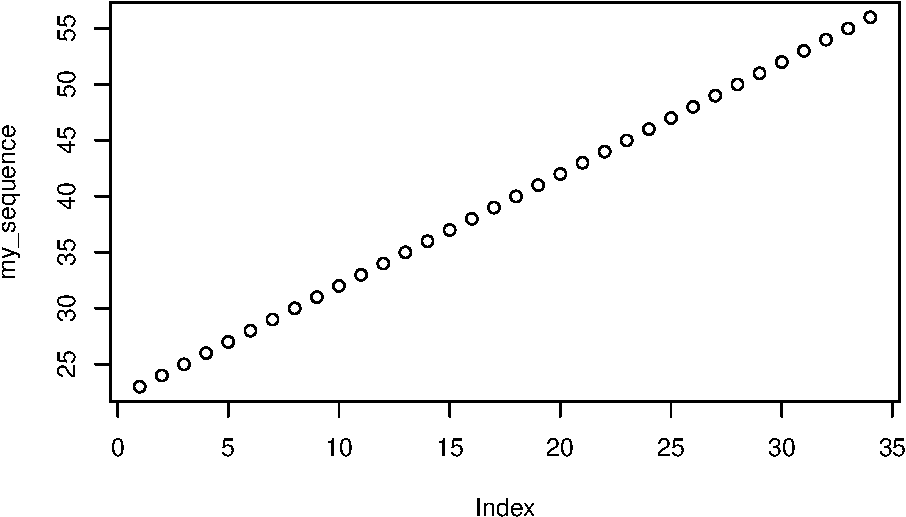
\includegraphics{Programming_Crump_files/figure-latex/unnamed-chunk-44-1.pdf}

The variable \emph{my\_sequence} contains the numbers 23 to 56, going up
by one. We see in the plot, the first number (on the x-axis) is a 23 on
the y-axis. As we go across the x-axis, the numbers go up by one until
we get to 56. We see a straight diagonal line.

\begin{Shaded}
\begin{Highlighting}[]
\KeywordTok{plot}\NormalTok{(my_randoms)}
\end{Highlighting}
\end{Shaded}

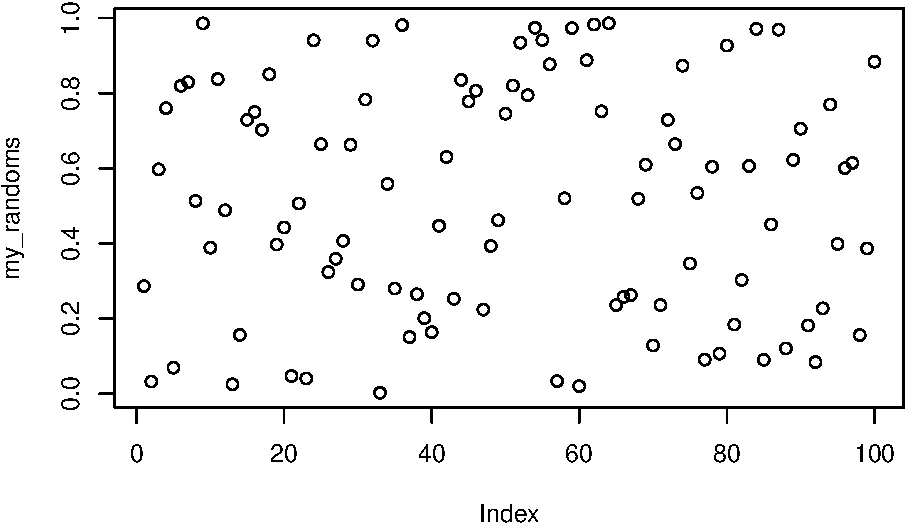
\includegraphics{Programming_Crump_files/figure-latex/unnamed-chunk-45-1.pdf}

The variable \emph{my\_randoms} contains 100 random numbers between 0
and 1. The plot shows dots all over the place between 0 and 1 on the
y-axis.

\begin{Shaded}
\begin{Highlighting}[]
\KeywordTok{plot}\NormalTok{(my_normal)}
\end{Highlighting}
\end{Shaded}

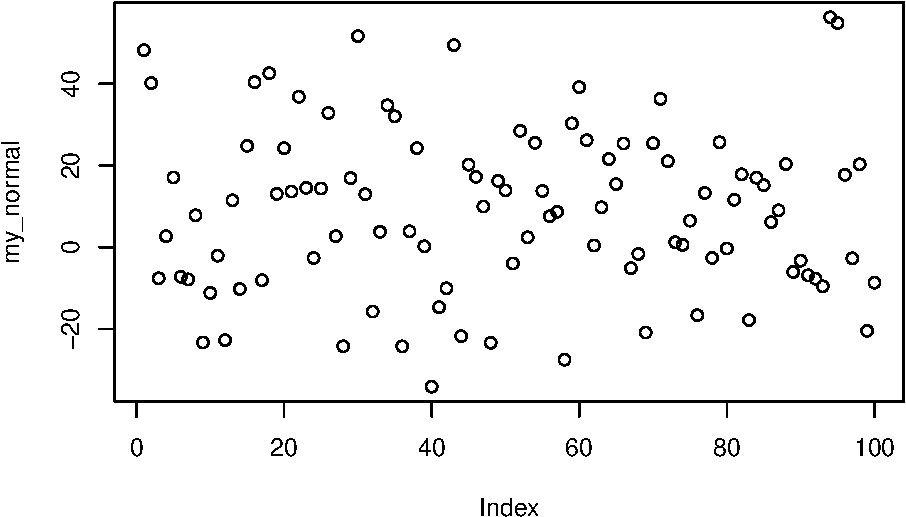
\includegraphics{Programming_Crump_files/figure-latex/unnamed-chunk-46-1.pdf}

The variable \emph{my\_normal} contains 100 numbers sample from a normal
distribution with a mean of 10, and a standard deviation of 20. Roughly,
most of the numbers should be close to 10, some of the numbers will be
greater and smaller than 10. But, as the numbers move away from 10 in
either direction, really small or really big numbers should occur less
and less frequently. We can sort of see this in the plot. For example,
you might notice that most the numbers are near the horizontal middle of
the graph, near the 10 on the y-axis, and less of the numbers are near
the top or bottom of the graph.

\subsubsection{Histograms}\label{histograms}

Histograms are used to visually summarize a set of numbers. In
particular, histograms split a set of numbers into bins, and then show
how many numbers fall within each bin. Each bin represents a pre-defined
range.

Let's create a set of numbers made up from 1s, 2s, and 3s. Let's say we
have ten 1s, twenty 2s, and 30 3s.

\begin{Shaded}
\begin{Highlighting}[]
\NormalTok{my_set <-}\StringTok{ }\KeywordTok{c}\NormalTok{(}\KeywordTok{rep}\NormalTok{(}\DecValTok{1}\NormalTok{,}\DecValTok{10}\NormalTok{),}\KeywordTok{rep}\NormalTok{(}\DecValTok{2}\NormalTok{,}\DecValTok{20}\NormalTok{),}\KeywordTok{rep}\NormalTok{(}\DecValTok{3}\NormalTok{,}\DecValTok{30}\NormalTok{))}
\end{Highlighting}
\end{Shaded}

The above line of code uses two R functions, rep(), and c(). We already
know how rep works. The c() function is short for combine. So, the above
line of code, combines 10 1s, 20 2s and 30 3s, all into one variable.
The contents of the variable looks like this:

\begin{Shaded}
\begin{Highlighting}[]
\NormalTok{my_set}
\end{Highlighting}
\end{Shaded}

\begin{verbatim}
##  [1] 1 1 1 1 1 1 1 1 1 1 2 2 2 2 2 2 2 2 2 2 2 2 2 2 2 2 2 2 2 2 3 3 3 3 3
## [36] 3 3 3 3 3 3 3 3 3 3 3 3 3 3 3 3 3 3 3 3 3 3 3 3 3
\end{verbatim}

Because, we made this variable, we already know what is inside it. Let's
make a histogram of the variable, to see what that looks like:

\begin{Shaded}
\begin{Highlighting}[]
\KeywordTok{hist}\NormalTok{(my_set)}
\end{Highlighting}
\end{Shaded}

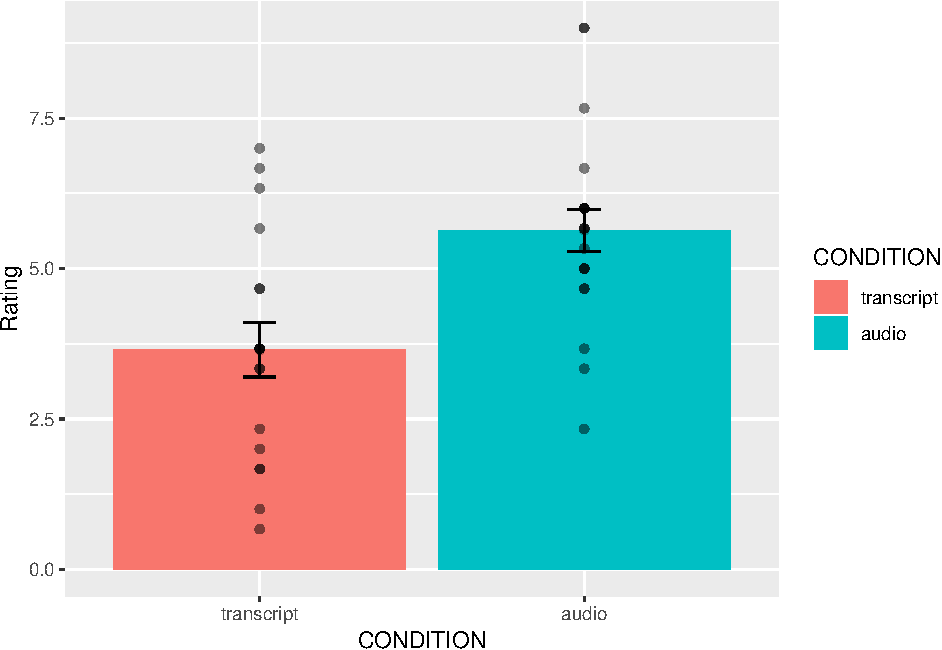
\includegraphics{Programming_Crump_files/figure-latex/unnamed-chunk-49-1.pdf}

The histogram is a bar graph. The height of each bar represents a count,
or the frequency of how many numbers fall inside each bin. The x-axis
shows the bin ranges. If you do not specify the bin ranges, then R will
make a reasonable guess for you. In this case, R set the bin ranges in
steps of .5. For example, 1-1.5, 1.5-2, 2-2.5, 2.5-3. R uses the word
\emph{breaks} to refer to bins. And, when you plot a histogram, you can
set your own breaks, or bin ranges.

\begin{Shaded}
\begin{Highlighting}[]
\KeywordTok{hist}\NormalTok{(my_set, }\DataTypeTok{breaks=}\KeywordTok{c}\NormalTok{(}\DecValTok{0}\NormalTok{,}\DecValTok{1}\NormalTok{,}\DecValTok{2}\NormalTok{,}\DecValTok{3}\NormalTok{,}\DecValTok{4}\NormalTok{))}
\end{Highlighting}
\end{Shaded}

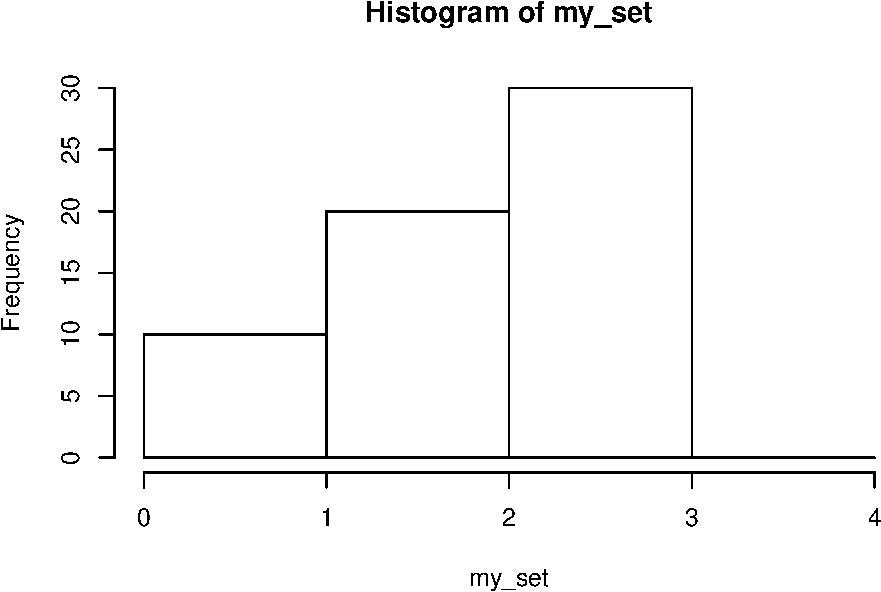
\includegraphics{Programming_Crump_files/figure-latex/unnamed-chunk-50-1.pdf}

Let's spend a moment interpreting this new histogram. The first bar is
between 0 and 1 on the x-axis, and has a value of 10 on the y-axis. This
means that there are 10 numbers inside the my\_set variable that have a
value between 0 and 1; specifically, a value greater than zero up to and
equalling 1. The second bar is between 1 and 2 on the x-axis, and has a
value of 20 on the y-axis. So, there are 20 numbers in the variable with
a value greater than 1 up to and equalling 2. Finally, the third bar
shows there are 30 numbers in the range greater than 2, up to equalling
3. We can also see there are no numbers smaller than 0, or greater than
4.

\subsubsection{What are histograms useful
for?}\label{what-are-histograms-useful-for}

A primary purpose of histograms is to get a quick look at the range and
frequency of a set of numbers. In particular, when the bars are of
different sizes, we can know that some values occur more than others.

What should a histogram look like for a set of values whose numbers all
occur randomly, and equally frequently? By this definition, we are
saying that all numbers, within all ranges, occur equally often. For
example, imagine we created a set of 10,000 numbers, and chose those
numbers from between 1 and 10, such that any number between 1 and 10
occurs with the same frequency as all other numbers. We can use the
random number generator and histogram to find out:

\begin{Shaded}
\begin{Highlighting}[]
\NormalTok{some_random_numbers <-}\StringTok{ }\KeywordTok{runif}\NormalTok{(}\DecValTok{10000}\NormalTok{,}\DecValTok{1}\NormalTok{,}\DecValTok{10}\NormalTok{)}
\KeywordTok{hist}\NormalTok{(some_random_numbers,}\DataTypeTok{breaks=}\KeywordTok{seq}\NormalTok{(}\DecValTok{0}\NormalTok{,}\DecValTok{11}\NormalTok{,}\DecValTok{1}\NormalTok{))}
\end{Highlighting}
\end{Shaded}

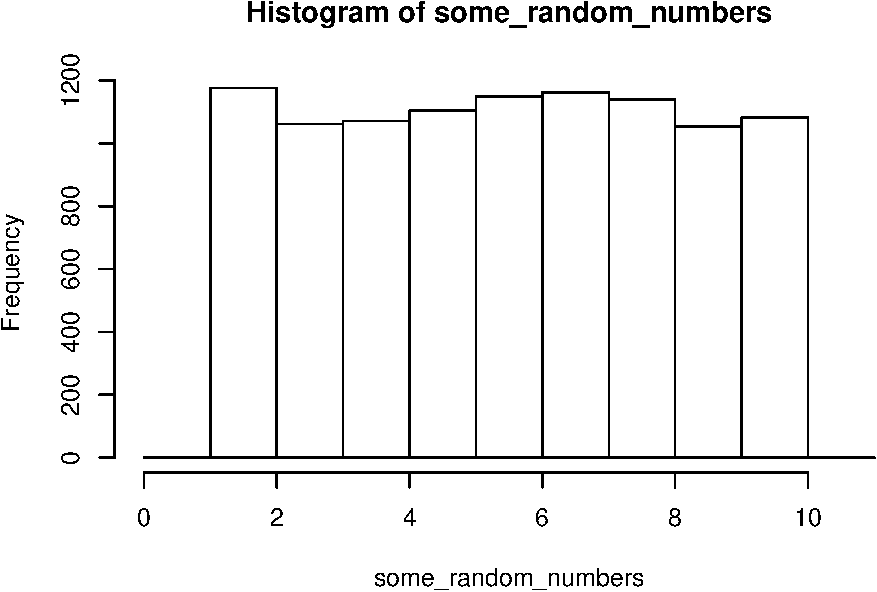
\includegraphics{Programming_Crump_files/figure-latex/unnamed-chunk-51-1.pdf}

\begin{Shaded}
\begin{Highlighting}[]
\CommentTok{#notice I set the breaks using the seq() function}
\end{Highlighting}
\end{Shaded}

We see that heights of the bars are all close to the same number. This
is good, because each number between 1 to 10 should have had an equal
chance of being selected. However, notice the bars are not exactly the
same height. This shows that the random number generator did actually
generate each number with equal frequency.

What about sets of numbers where some kinds of numbers occur more than
others? Here, we would expect higher bars for ranges containing many
values, and smaller numbers for ranges containing fewer values.

Let's plot histogram for a normal distribution and see what it looks
like. We will set the mean to 100, and the standard deviation to 20, and
we ask R to generate 10000 numbers from this distribution.

\begin{Shaded}
\begin{Highlighting}[]
\NormalTok{normal_sample <-}\StringTok{ }\KeywordTok{rnorm}\NormalTok{(}\DecValTok{10000}\NormalTok{,}\DecValTok{100}\NormalTok{,}\DecValTok{20}\NormalTok{)}
\KeywordTok{hist}\NormalTok{(normal_sample)}
\end{Highlighting}
\end{Shaded}

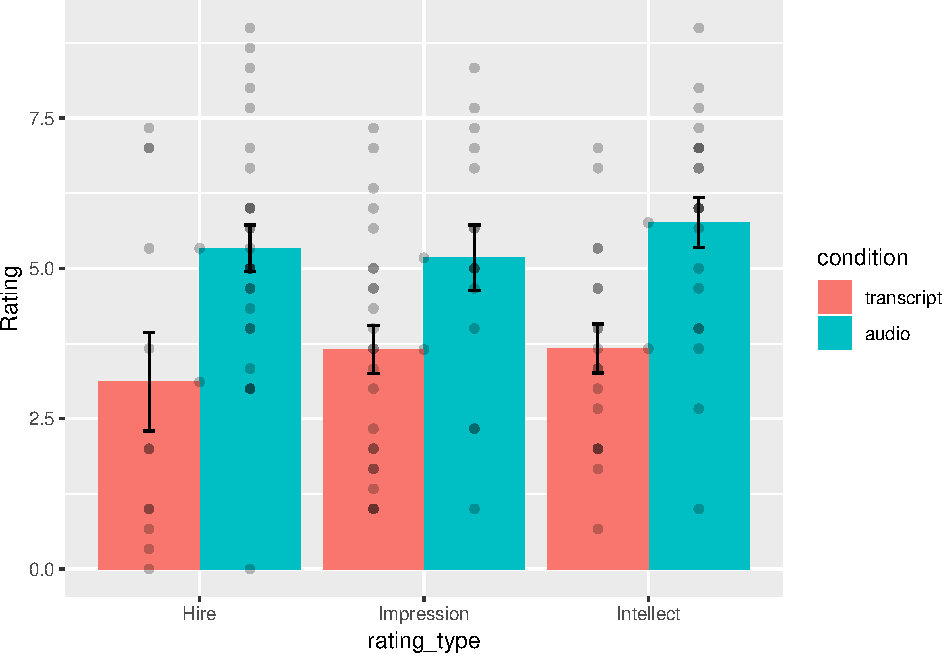
\includegraphics{Programming_Crump_files/figure-latex/unnamed-chunk-52-1.pdf}
The histogram shows that the highest bars are in the middle, near the
100 mark. So, numbers near 100 occured most frequently in our set. What
happens to the heights of the bars on either side of the histogram? The
bars are decreasing in height as they move away from the middle in both
directions. So, as numbers move away from 100, they occur less and less
frequently. For example, we don't see any bars in the range of 500 or
1000. This means that no values that high were in our set of numbers.
From the histogram, we can clearly see that our set hardly had any
numbers greater than 150, or less than 50. Or, in other words, most of
the numbers were between 50 and 150.

--\textgreater{}

\section{Excel}\label{excel}

\section{SPSS}\label{spss}

\section{Matlab}\label{matlab}

\chapter{Lab 2: Descriptive
Statistics}\label{lab-2-descriptive-statistics}

{ Some inspiring quote ---Inspiring Person }

\section{Outline of Problem to solve}\label{outline-of-problem-to-solve}

Stuff we need to say in general

\subsection{important things}\label{important-things}

Other things to say

\section{R}\label{r-2}

How to do it in R

\section{Excel}\label{excel-1}

How to do it in Excel

\section{SPSS}\label{spss-1}

How to do it in SPSS

\section{Matlab}\label{matlab-1}

How to do it in Matlab

\chapter{Lab 3: Correlation}\label{lab-3-correlation}

{ Some inspiring quote ---Inspiring Person }

\section{Outline of Problem to
solve}\label{outline-of-problem-to-solve-1}

Stuff we need to say in general

\subsection{important things}\label{important-things-1}

Other things to say

\section{R}\label{r-3}

How to do it in R

\section{Excel}\label{excel-2}

How to do it in Excel

\section{SPSS}\label{spss-2}

How to do it in SPSS

\section{Matlab}\label{matlab-2}

How to do it in Matlab

\chapter{Lab 4: Normal Distribution \& Central Limit
Theorem}\label{lab-4-normal-distribution-central-limit-theorem}

{ Some inspiring quote ---Inspiring Person }

\section{Outline of Problem to
solve}\label{outline-of-problem-to-solve-2}

Stuff we need to say in general

\subsection{important things}\label{important-things-2}

Other things to say

\section{R}\label{r-4}

How to do it in R

\section{Excel}\label{excel-3}

How to do it in Excel

\section{SPSS}\label{spss-3}

How to do it in SPSS

\section{Matlab}\label{matlab-3}

How to do it in Matlab

\chapter{Lab 5: Fundamentals of Hypothesis
Testing}\label{lab-5-fundamentals-of-hypothesis-testing}

{ Some inspiring quote ---Inspiring Person }

\section{Outline of Problem to
solve}\label{outline-of-problem-to-solve-3}

Stuff we need to say in general

\subsection{important things}\label{important-things-3}

Other things to say

\section{R}\label{r-5}

How to do it in R

\section{Excel}\label{excel-4}

How to do it in Excel

\section{SPSS}\label{spss-4}

How to do it in SPSS

\section{Matlab}\label{matlab-4}

How to do it in Matlab

\chapter{Lab 6: t-Test (one-sample, paired
sample)}\label{lab-6-t-test-one-sample-paired-sample}

This lab is modified and extended from
\href{https://sites.trinity.edu/osl}{Open Stats Labs}. Thanks to Open
Stats Labs (Dr.~Kevin P. McIntyre) for their fantastic work.

\section{Does Music Convey Social Information to
Infants?}\label{does-music-convey-social-information-to-infants}

This lab activity uses the open data from Experiment 1 of Mehr, Song,
and Spelke (2016) to teach one-sample and paired samplest -tests.
Results of the activity provided below should exactly reproduce the
results described in the paper.

\subsection{STUDY DESCRIPTION}\label{study-description}

Parents often sing to their children and, even as infants, children
listen to and look at their parents while they are singing.Research by
Mehr, Song, and Spelke (2016) sought to explore the psychological
function that music has for parents and infants, by examining the
hypothesis that particular melodies convey important social information
to infants.Specifically, melodies convey information about social
affiliation.

The authors argue that melodies are shared within social groups. Whereas
children growing up in one culture may be exposed to certain songs as
infants (e.g., ``Rock-a-bye Baby''), children growing up in other
cultures (or even other groups within a culture) may be exposed to
different songs.Thus, when a novel person (someone who the infant has
never seen before) sings a familiar song, it may signal to the infant
that this new person is a member of their social group.

To test this hypothesis, the researchers recruited 32 infants and their
parents to complete an experiment.During their first visit to the lab,
the parents were taught a new lullaby (one that neither they nor their
infants had heard before).The experimenters asked the parents to sing
the new lullaby to their child every day for the next 1-2 weeks.

Following this 1-2 week exposure period, the parents and their infant
returned to the lab to complete the experimental portion of the
study.Infants were first shown a screen with side-by-side videos of two
unfamiliar people, each of whom were silently smiling and looking at the
infant.The researchers recorded the looking behavior (or gaze) of the
infants during this `baseline' phase. Next, one by one, the two
unfamiliar people on the screen sang either the lullaby that the parents
learned or a different lullaby (that had the same lyrics and rhythm, but
a different melody).Finally, the infants saw the same silent video used
at baseline, and the researchers again recorded the looking behavior of
the infants during this `test' phase.For more details on the
experiment's methods, please refer to Mehr et al. (2016) Experiment 1.

\section{Lab skills learned}\label{lab-skills-learned}

\begin{enumerate}
\def\labelenumi{\arabic{enumi}.}
\tightlist
\item
  Conducting a one-sample t-test
\item
  Conducting a two-sample t-test
\item
  Plotting the data
\item
  Discussing inferences and limitations
\end{enumerate}

\section{Important Stuff}\label{important-stuff}

\begin{itemize}
\tightlist
\item
  citation: Mehr, S. A., Song. L. A., \& Spelke, E. S. (2016). For
  5-month-old infants, melodies are social. Psychological Science, 27,
  486-501.
\item
  \href{http://journals.sagepub.com/stoken/default+domain/d5HcBHg85XamSXGdYqYN/full}{Link
  to .pdf of article}
\item
  \href{https://drive.google.com/open?id=0Bz-rhZ21ShvOdW1wV0pmUTJSSk0}{Data
  in .csv format}
\item
  \href{https://drive.google.com/open?id=0Bz-rhZ21ShvOa3c4X3hqOWxwcUU}{Data
  in SPSS format}
\end{itemize}

\section{R}\label{r-6}

\subsection{Loading the data}\label{loading-the-data}

The first thing to do is download the .csv formatted data file, using
the link above, or just click
\href{https://drive.google.com/open?id=0Bz-rhZ21ShvOdW1wV0pmUTJSSk0}{here}.
It turns out there are lots of ways to load .csv files into R.

\begin{enumerate}
\def\labelenumi{\arabic{enumi}.}
\tightlist
\item
  Load the data.table library. Then use the fread function and supply
  the web address to the file. Just like this. No downloading required.
\end{enumerate}

\begin{Shaded}
\begin{Highlighting}[]
\KeywordTok{library}\NormalTok{(data.table)}
\NormalTok{all_data <-}\StringTok{ }\KeywordTok{fread}\NormalTok{(}\StringTok{"https://raw.githubusercontent.com/CrumpLab/statisticsLab/master/data/MehrSongSpelke2016.csv"}\NormalTok{)}
\end{Highlighting}
\end{Shaded}

\begin{enumerate}
\def\labelenumi{\arabic{enumi}.}
\setcounter{enumi}{1}
\tightlist
\item
  Or, if you downloaded the .csv file. Then you can use fread, but you
  need to point it to the correct file location. The file location in
  this next example will not work for you, because the file is on my
  computer.
\end{enumerate}

\begin{Shaded}
\begin{Highlighting}[]
\KeywordTok{library}\NormalTok{(data.table)}
\NormalTok{all_data <-}\StringTok{ }\KeywordTok{fread}\NormalTok{(}\StringTok{"Data/MehrSongSpelke2016.csv"}\NormalTok{)}
\end{Highlighting}
\end{Shaded}

\subsection{Inspect the data frame}\label{inspect-the-data-frame}

When you have loaded data it's always a good idea to check out what it
looks like. You can look at all of the data in the environment tab on
the top right hand corner. The data should be in a variable called
\texttt{all\_data}. Clicking on \texttt{all\_data} will load it into a
viewer, and you can scroll around. This can be helpful to see things.
But, there is so much data, can be hard to know what you are looking
for.

\subsubsection{summarytools}\label{summarytools-1}

The summarytools packages give a quick way to summarize all of the data
in a data frame. Here's how. When you run this code you will see the
summary in the viewer on the bottom right hand side. There's a little
browser button (arrow on top of little window) that you can click to
expand and see the whole thing in a browser.

\begin{Shaded}
\begin{Highlighting}[]
\KeywordTok{library}\NormalTok{(summarytools)}
\KeywordTok{view}\NormalTok{(}\KeywordTok{dfSummary}\NormalTok{(all_data))}
\end{Highlighting}
\end{Shaded}

\subsection{Get the data for Experiment
one}\label{get-the-data-for-experiment-one}

The data contains all of the measurements from all five experiments in
the paper. By searching through the \texttt{all\_data} dataframe, you
should look for the variables that code for each experiment. For
example, the third column is called \texttt{exp1}, which stands for
experiment 1. Notice that it contains a series of 1s. If you keep
scrolling down, the 1s stop. These 1s identify the rows associated with
the data for Experiment 1. We only want to analyse that data. So, we
need to filter our data, and put only those rows into a new variable. We
do this with the \texttt{dplyr} library, using the \texttt{filter}
function.

\begin{Shaded}
\begin{Highlighting}[]
\KeywordTok{library}\NormalTok{(dplyr)}
\NormalTok{experiment_one <-}\StringTok{ }\NormalTok{all_data %>%}\StringTok{ }\KeywordTok{filter}\NormalTok{(exp1==}\DecValTok{1}\NormalTok{)}
\end{Highlighting}
\end{Shaded}

Now if you look at the new variable \texttt{experiment\_one}, there are
only 32 rows of data. Much less than before. Now we have the data from
experiment 1.

\subsection{Baseline phase: Conduct a one sample
t-test}\label{baseline-phase-conduct-a-one-sample-t-test}

You first want to show that infants' looking behavior did not differ
from chance during the baseline trial. The baseline trial was 16 seconds
long. During the baseline, infants watched a video of two unfamilar
people, one of the left and one on the right. There was no sound during
the basline. Both of the actors in the video smiled directly at the
infant.

The important question was to determine whether the infant looked more
or less to either person. If they showed no preference, the infant
should look at both people about 50\% of the time. How could we
determine whether the infant looked at both people about 50\% of the
time?

The \texttt{experiment\_one} dataframe has a column called
\texttt{Baseline\_Proportion\_Gaze\_to\_Singer}. All of these values
show how the proportion of time that the infant looked to the person who
would later sing the familiar song to them. If the average of these
proportion is .5 across the infants, then we would have some evidence
that the infants were not biased at the beginning of the experiment.
However, if the infants on average had a bias toward the singer, then
the average proportion of the looking time should be different than .5.

Using a one-sample t-test, we can test the hypothesis that our sample
mean for the \texttt{Baseline\_Proportion\_Gaze\_to\_Singer} was not
different from .5.

To do this in R, we just need to isolate the column of data called
\texttt{Baseline\_Proportion\_Gaze\_to\_Singer}. We will do this using
the \texttt{\$} operator. The \texttt{\$} operator is placed after any
data frame variable, and allows you to select a column of the data. The
next bit of code will select the column of data we want, and put it into
a new variable called \texttt{Baseline}. Note, if you type
\texttt{exp1\$} then Rstudio should automatically bring up all the
columns you can choose from.

\begin{Shaded}
\begin{Highlighting}[]
\NormalTok{baseline <-}\StringTok{ }\NormalTok{experiment_one$Baseline_Proportion_Gaze_to_Singer}
\end{Highlighting}
\end{Shaded}

\subsubsection{Look at the numbers}\label{look-at-the-numbers}

\textbf{Question:} Why is it important to look at your numbers? What
could happen if you didn't?

Ok, we could just do the t-test right away, it's really easy, only one
line of code. But, we haven't even looked at the numbers yet. Let's at
least do that. First, we'll just use plot. It will show every data point
for each infant as a dot.

\begin{Shaded}
\begin{Highlighting}[]
\KeywordTok{plot}\NormalTok{(baseline)}
\end{Highlighting}
\end{Shaded}

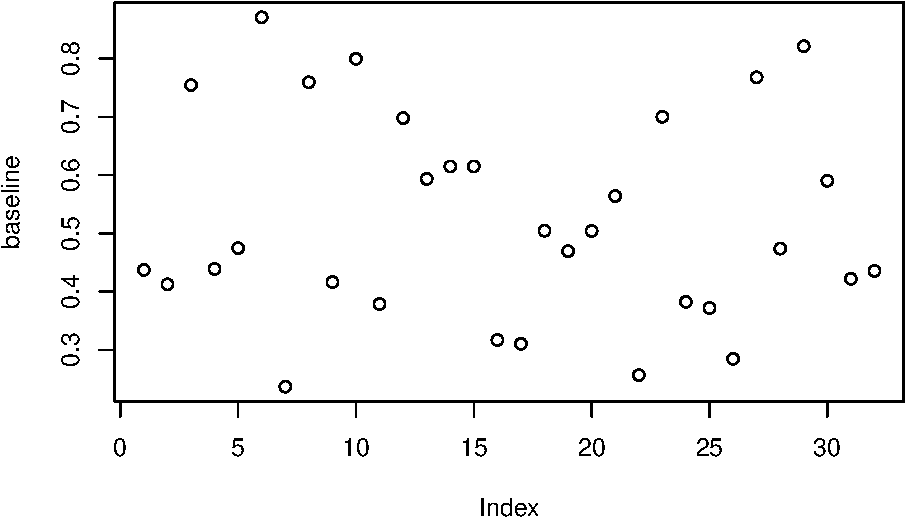
\includegraphics{Programming_Crump_files/figure-latex/unnamed-chunk-58-1.pdf}

That's helpful, we see that the dots are all over the place. Let's do a
histrogram, so we can get a better sense of the frequency of different
proportions.

\begin{Shaded}
\begin{Highlighting}[]
\KeywordTok{hist}\NormalTok{(baseline)}
\end{Highlighting}
\end{Shaded}

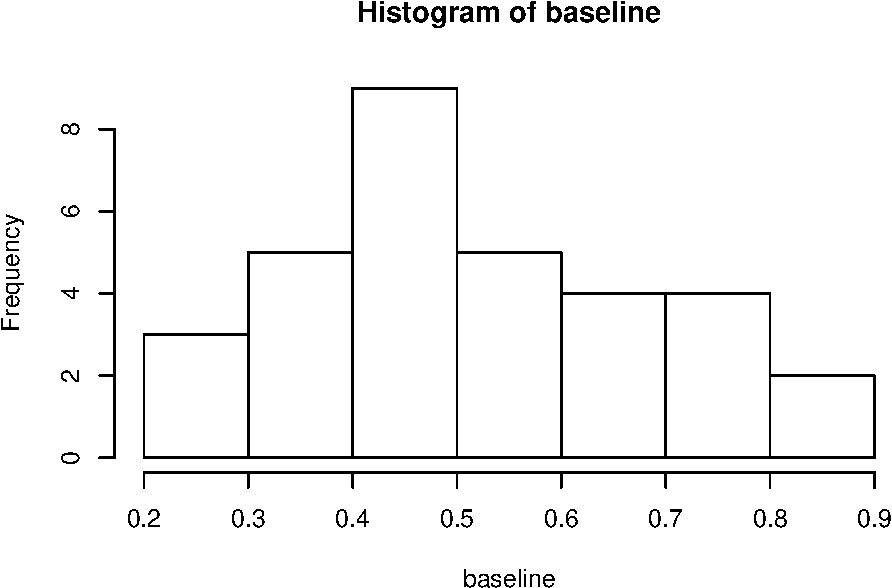
\includegraphics{Programming_Crump_files/figure-latex/unnamed-chunk-59-1.pdf}

\subsubsection{Look at the descriptives}\label{look-at-the-descriptives}

Let's get the mean and standard deviation of the sample

\begin{Shaded}
\begin{Highlighting}[]
\KeywordTok{mean}\NormalTok{(baseline)}
\end{Highlighting}
\end{Shaded}

\begin{verbatim}
## [1] 0.5210967
\end{verbatim}

\begin{Shaded}
\begin{Highlighting}[]
\KeywordTok{sd}\NormalTok{(baseline)}
\end{Highlighting}
\end{Shaded}

\begin{verbatim}
## [1] 0.1769651
\end{verbatim}

Ok, so just looking at the mean, we see the proportion is close to .5
(it's .521). And, we see there is a healthy amount of variance (the dots
were all over the place), as the standard deviation was about .176.

\textbf{Question:} Based on the means and standard deviations can you
make an educated guess about what the t and p values might be? Learn how
to do this and you will be improving your data-sense.

Now, before we run the t-test, what do you think is going to happen? We
are going to get a t-value, and an associated p-value. If you can make a
guess at what those numbers would be right now in your head, and those
end up being pretty close to the ones we will see in a moment, then you
should pat yourself on the back. You have learned how to have intuitions
about the data. As I am writing this I will tell you that 1) I can't
remember what the t and p was from the paper, and I haven't done the
test yet, so I don't know the answer. So, I am allowed to guess what the
answer will be. Here are my guesses t(31) = 0.2, p = .95. The numbers in
the brackets are degrees of freedom, which we know are 31 (df= n-1 =
32-1= 31). More important than the specific numbers I am guessing (which
will probably be wrong), I am guessing that the p-value will be pretty
large, it will not be less than .05, which the author's set as their
alpha rate. So, I am guessing we will not reject the hypothesis that .52
is different from .5.

Let's do the t-test and see what happens.

\subsubsection{Conduct t.test}\label{conduct-t.test}

\begin{Shaded}
\begin{Highlighting}[]
\KeywordTok{t.test}\NormalTok{(baseline, }\DataTypeTok{mu=}\NormalTok{.}\DecValTok{5}\NormalTok{)}
\end{Highlighting}
\end{Shaded}

\begin{verbatim}
## 
##  One Sample t-test
## 
## data:  baseline
## t = 0.67438, df = 31, p-value = 0.5051
## alternative hypothesis: true mean is not equal to 0.5
## 95 percent confidence interval:
##  0.4572940 0.5848994
## sample estimates:
## mean of x 
## 0.5210967
\end{verbatim}

\textbf{Question:} Why was the baseline condition important for the
experiment? What does performance in this condition tell us?

So, there we have it. We did a one-sample t-test. Here's how you would
report it, t(31) = .67, p = .505. Or, we might say something like:

\begin{quote}
During the baseline condition, the mean proportion looking time toward
the singer was .52, and was not significantly different from .5,
according to a one-sample test, t(31) = .67, p = .505.
\end{quote}

You should take the time to check this result, and see if it is the same
one that was reported in the paper.

\subsection{Test phase}\label{test-phase}

Remember how the experiment went. Infants watched silent video
recordings of two women (Baseline). Then each person sung a song, one
was familiar to the infant (their parents sung the song to them many
times), and one was unfamiliar (singing phase). After the singing phase,
the infants watched the silent video of the two singers argain (test
phase). The critical question was whether the infants would look more to
the person who sung the familiar song compared to the person who sun the
unfamiliar song. If the infants did this, they should look more than
50\% of the time to the singer who sang the familiar song. We have the
data, we can do another one sample t-test to find out. We can re-use all
the code we already wrote to do this. I'll put it all in one place. If
we run all of this code, we will see all of the things we want to see.

We only need to make two changes. We will change
\texttt{experiment\_one\$Baseline\_Proportion\_Gaze\_to\_Singer} to
\texttt{experiment\_one\$Test\_Proportion\_Gaze\_to\_Singer}, because
that column has the test phase data. And, instead of putting the data
into the variable \texttt{baseline}. We will make a new variable called
\texttt{test\_phase} to store the data.

\begin{Shaded}
\begin{Highlighting}[]
\NormalTok{test_phase <-}\StringTok{ }\NormalTok{experiment_one$Test_Proportion_Gaze_to_Singer}
\KeywordTok{plot}\NormalTok{(test_phase)}
\end{Highlighting}
\end{Shaded}

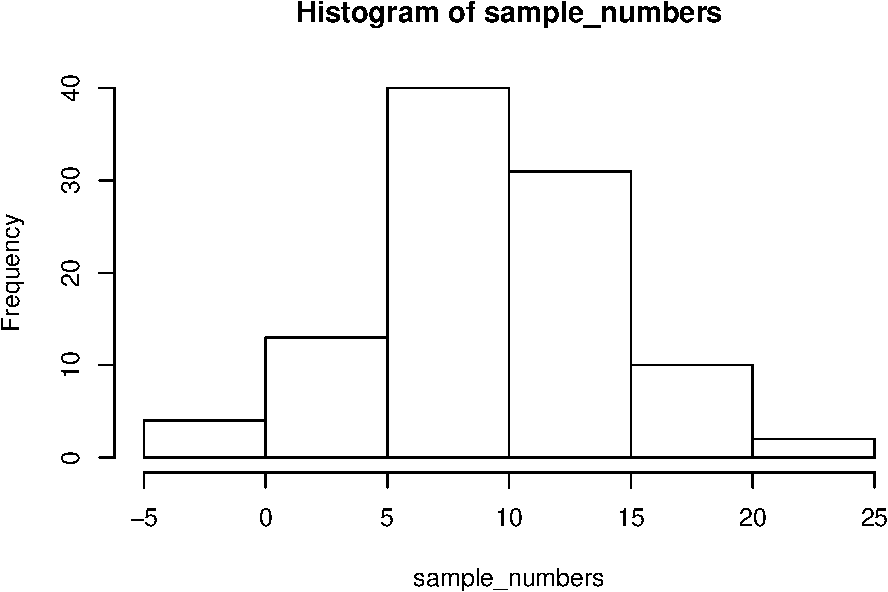
\includegraphics{Programming_Crump_files/figure-latex/unnamed-chunk-62-1.pdf}

\begin{Shaded}
\begin{Highlighting}[]
\KeywordTok{hist}\NormalTok{(test_phase)}
\end{Highlighting}
\end{Shaded}

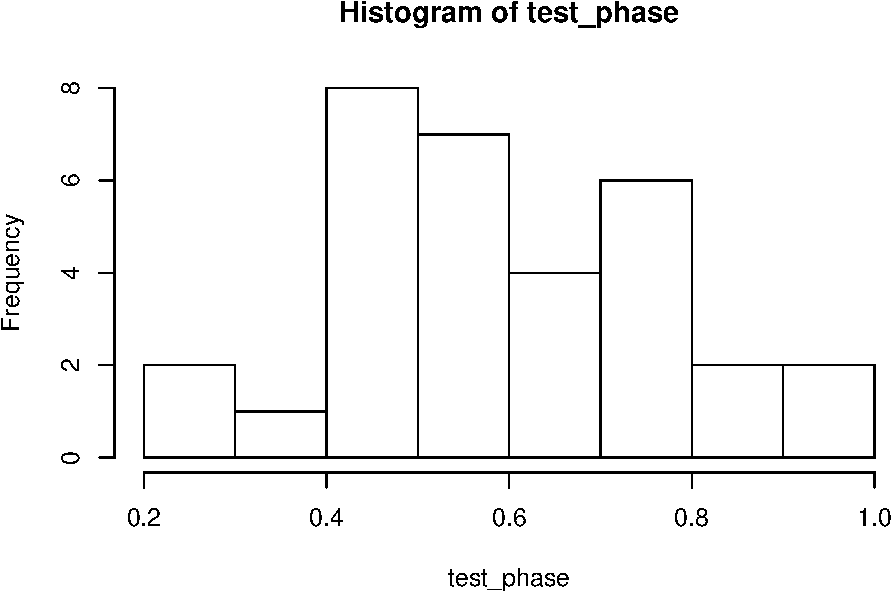
\includegraphics{Programming_Crump_files/figure-latex/unnamed-chunk-62-2.pdf}

\begin{Shaded}
\begin{Highlighting}[]
\KeywordTok{mean}\NormalTok{(test_phase)}
\end{Highlighting}
\end{Shaded}

\begin{verbatim}
## [1] 0.5934913
\end{verbatim}

\begin{Shaded}
\begin{Highlighting}[]
\KeywordTok{sd}\NormalTok{(test_phase)}
\end{Highlighting}
\end{Shaded}

\begin{verbatim}
## [1] 0.1786884
\end{verbatim}

\begin{Shaded}
\begin{Highlighting}[]
\KeywordTok{t.test}\NormalTok{(test_phase, }\DataTypeTok{mu =} \NormalTok{.}\DecValTok{5}\NormalTok{)}
\end{Highlighting}
\end{Shaded}

\begin{verbatim}
## 
##  One Sample t-test
## 
## data:  test_phase
## t = 2.9597, df = 31, p-value = 0.005856
## alternative hypothesis: true mean is not equal to 0.5
## 95 percent confidence interval:
##  0.5290672 0.6579153
## sample estimates:
## mean of x 
## 0.5934913
\end{verbatim}

\textbf{Question:} Why was the test condition important for the
experiment? What does performance in this condition tell us?

Alright. What did we find? You should take a stab at writing down what
we found. You can use the same kind of language that I used from the
first one sample-test. You should state the mean proportion, the
t-value, the dfs, and the p-value. You should be able to answer the
question, did the infants look longer at the singer who sang the
familiar song? And, did they look longer than would be consist with
chance at 50\%.

\subsection{Paired-samples t-test}\label{paired-samples-t-test}

The paired samples t-test is easy to do. We've already made two
variables called \texttt{baseline}, and \texttt{test\_phase}. These
contain each of the infants looking time proportions to the singer for
both parts of the experiment. We can see if the difference between them
was likely or unlikely due to chance by running a paired samples t-test.
We do it like this in one line:

\begin{Shaded}
\begin{Highlighting}[]
\KeywordTok{t.test}\NormalTok{(test_phase, baseline, }\DataTypeTok{paired=}\OtherTok{TRUE}\NormalTok{, }\DataTypeTok{var.equal=}\OtherTok{TRUE}\NormalTok{)}
\end{Highlighting}
\end{Shaded}

\begin{verbatim}
## 
##  Paired t-test
## 
## data:  test_phase and baseline
## t = 2.4164, df = 31, p-value = 0.02175
## alternative hypothesis: true difference in means is not equal to 0
## 95 percent confidence interval:
##  0.01129217 0.13349698
## sample estimates:
## mean of the differences 
##              0.07239458
\end{verbatim}

\textbf{Question:} Why was the paired samples t-test necessary if we
already did two one sample t-test? What new question is the paired
samples t-test asking?

I'l leave it to you to interpret these values, and to see if they are
the same as the ones in the paper. Based on these values what do you
conclude? Is there a difference between the mean proportion looking
times for the baseline and testing phase?

\subsubsection{Relationship between one-sample and paired sample
t-test}\label{relationship-between-one-sample-and-paired-sample-t-test}

\textbf{Question:} Why is it that a paired samples t-test can be the
same as the one sample t-test? What do you have to do the data in the
paired samples t-test in order to conduct a one-sample t-test that would
give you the same result?

We've discussed in the textbook that the one-sample and paired sample
t-test are related, they can be the same test. The one-sample test
whether a sample mean is different from some particular mean. The paired
sample t-test, is to determine whether one sample mean is different from
another sample mean. If you take the scores for each variable in a
paired samples t-test, and subtract them from one another, then you have
one list of difference scores. Then, you could use a one sample t-test
to test whether these difference scores are different from 0. It turns
out you get the same answer from a paired sample t-test testing the
difference between two sample means, and the one sample t-test testing
whether the mean difference of the difference scores between the samples
are different from 0. We can show this in r easily like this:

\begin{Shaded}
\begin{Highlighting}[]
\KeywordTok{t.test}\NormalTok{(test_phase, baseline, }\DataTypeTok{paired=}\OtherTok{TRUE}\NormalTok{, }\DataTypeTok{var.equal=}\OtherTok{TRUE}\NormalTok{)}
\end{Highlighting}
\end{Shaded}

\begin{verbatim}
## 
##  Paired t-test
## 
## data:  test_phase and baseline
## t = 2.4164, df = 31, p-value = 0.02175
## alternative hypothesis: true difference in means is not equal to 0
## 95 percent confidence interval:
##  0.01129217 0.13349698
## sample estimates:
## mean of the differences 
##              0.07239458
\end{verbatim}

\begin{Shaded}
\begin{Highlighting}[]
\NormalTok{difference_scores<-test_phase-baseline}
\KeywordTok{t.test}\NormalTok{(difference_scores, }\DataTypeTok{mu=}\DecValTok{0}\NormalTok{)}
\end{Highlighting}
\end{Shaded}

\begin{verbatim}
## 
##  One Sample t-test
## 
## data:  difference_scores
## t = 2.4164, df = 31, p-value = 0.02175
## alternative hypothesis: true mean is not equal to 0
## 95 percent confidence interval:
##  0.01129217 0.13349698
## sample estimates:
##  mean of x 
## 0.07239458
\end{verbatim}

\subsubsection{Usefulness of difference
scores}\label{usefulness-of-difference-scores}

Ok fine, the paired samples t-test can be a one sample t-test if you use
the difference scores. This might just seem like a mildly useful factoid
you can use for stats trivia games (which no one plays). The point of
drawing your attention to the relationship, is to get you to focus on
the difference scores. These are what we are actually interested in.

Let's use the difference scores to one more useful thing. Sometime the
results of a t-test aren't intuitively obvious. By the t-test we found
out that a small difference between the test phase and baseline was not
likely produced by chance. How does this relate to the research question
about infants using familiar songs as cues for being social? Let's ask a
very simple question. How many infants actually showed the bias? How
many infants out of 32 looked longer at the singer who sang the familiar
song during test, compared to during baseline.

We can determine this by calculating the difference scores. Then, asking
how many of them were greater than zero:

\begin{Shaded}
\begin{Highlighting}[]
\NormalTok{difference_scores <-}\StringTok{ }\NormalTok{test_phase-baseline}
\KeywordTok{length}\NormalTok{(difference_scores[difference_scores>}\DecValTok{0}\NormalTok{])}
\end{Highlighting}
\end{Shaded}

\begin{verbatim}
## [1] 22
\end{verbatim}

So, 22 out of 32 infants showed the effect. To put that in terms of
probability, 68.75\% of infants showed the effect. These odds and
percentages give us another way to appreciate how strong the effect is.
It wasn't strong enough for all infants to show it.

\subsection{Graphing the findings}\label{graphing-the-findings}

It is often useful to graph the results of our analysis. We have already
looked at dot plots and histograms of the individual samples. But, we
also conducted some t-tests on the means of the baseline and test\_phase
samples. One of the major questions was whether these means are
different. Now, we will make a graph that shows the means for each
condition. Actually, we will make a few different graphs, so that you
can think about what kinds of graphs are most helpful. There are two
major important things to show: 1) the sample means, and 2) a visual aid
for statistical inference showing whether the results were likely due to
chance.

We will use the ggplot2 package to make our graphs. Remember, there are
two steps to take when using ggplot2. 1) put your data in a long form
dataframe, where each measure has one row, and 2) define the layers of
the ggplot.

\subsubsection{Make the dataframe for
plotting}\label{make-the-dataframe-for-plotting}

To start we will need 2 columns. One column will code the experimental
phase, Baseline or Test. There are 32 observations in each phase, so we
want the word \texttt{Baseline} to appear 32 times, followed by the word
\texttt{Test} 32 times. Then we want a single column with each of the
proportions for each infant.

\begin{Shaded}
\begin{Highlighting}[]
\NormalTok{Phase <-}\StringTok{ }\KeywordTok{rep}\NormalTok{(}\KeywordTok{c}\NormalTok{(}\StringTok{"Baseline"}\NormalTok{,}\StringTok{"Test"}\NormalTok{), }\DataTypeTok{each =} \DecValTok{32}\NormalTok{)}
\NormalTok{Proportions <-}\StringTok{ }\KeywordTok{c}\NormalTok{(baseline,test_phase)}
\NormalTok{plot_df <-}\StringTok{ }\KeywordTok{data.frame}\NormalTok{(Phase,Proportions)}
\end{Highlighting}
\end{Shaded}

\subsubsection{Dot plot of raw scores}\label{dot-plot-of-raw-scores}

This shows every scores value on the y-axis, split by the baseline and
test groups. If you just looked at this, you might not think the test
phase was different from the basline phase. Still very useful to see the
spread of individual scores. Supports the intuition that the scores are
still kind of in a similar ballpark.

\begin{Shaded}
\begin{Highlighting}[]
\KeywordTok{library}\NormalTok{(ggplot2)}
\KeywordTok{ggplot}\NormalTok{(plot_df, }\KeywordTok{aes}\NormalTok{(}\DataTypeTok{x=}\NormalTok{Phase, }\DataTypeTok{y=}\NormalTok{Proportions))+}
\StringTok{  }\KeywordTok{geom_point}\NormalTok{()}
\end{Highlighting}
\end{Shaded}

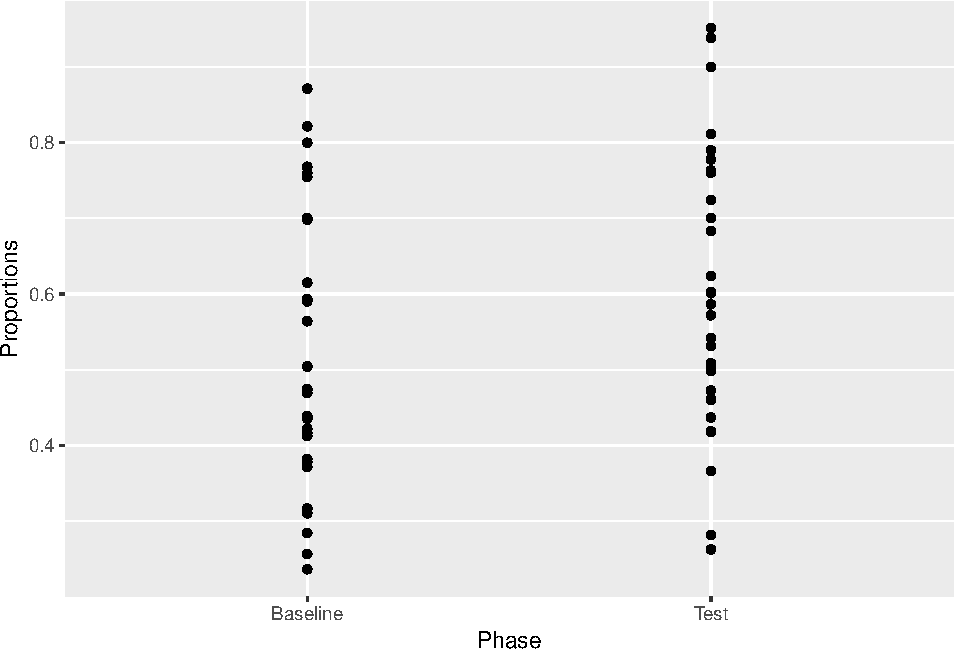
\includegraphics{Programming_Crump_files/figure-latex/unnamed-chunk-67-1.pdf}

\subsubsection{Dot plot with means and raw
scores}\label{dot-plot-with-means-and-raw-scores}

\textbf{Question:} What kinds of inferences about the role of chance in
producing the difference between the means can we make from this graph?
What is missing?

\texttt{ggplot2} is great because it let's us add different layers on
top of an existing plot. It would be good to see where the mean values
for each sample lie on top of the sample scores. We can do this. But, to
do it, we need to supply ggplot with another data frame, one that
contains the means for each phase in long form. There are are only two
phases, and two means, so we will make a rather small data.frame. It
will have two columns, a Phase column, and Mean\_value column. There
will only be two rows in the dataframe, one for the mean for each phase.

To make the smaller data frame for the means we will use the
\texttt{aggregate} function. This allows us to find the means for each
phase from the plot\_df dataframe. It also automatically returns the
data frame we are looking for.

\begin{Shaded}
\begin{Highlighting}[]
\NormalTok{mean_df <-}\StringTok{ }\KeywordTok{aggregate}\NormalTok{(Proportions ~}\StringTok{ }\NormalTok{Phase, plot_df, mean)}

\KeywordTok{ggplot}\NormalTok{(plot_df, }\KeywordTok{aes}\NormalTok{(}\DataTypeTok{x=}\NormalTok{Phase, }\DataTypeTok{y=}\NormalTok{Proportions))+}\StringTok{ }
\StringTok{  }\KeywordTok{geom_point}\NormalTok{()+}
\StringTok{  }\KeywordTok{geom_point}\NormalTok{(}\DataTypeTok{data=}\NormalTok{mean_df, }\DataTypeTok{color=}\StringTok{"Red"}\NormalTok{, }\DataTypeTok{size=}\DecValTok{2}\NormalTok{)}
\end{Highlighting}
\end{Shaded}

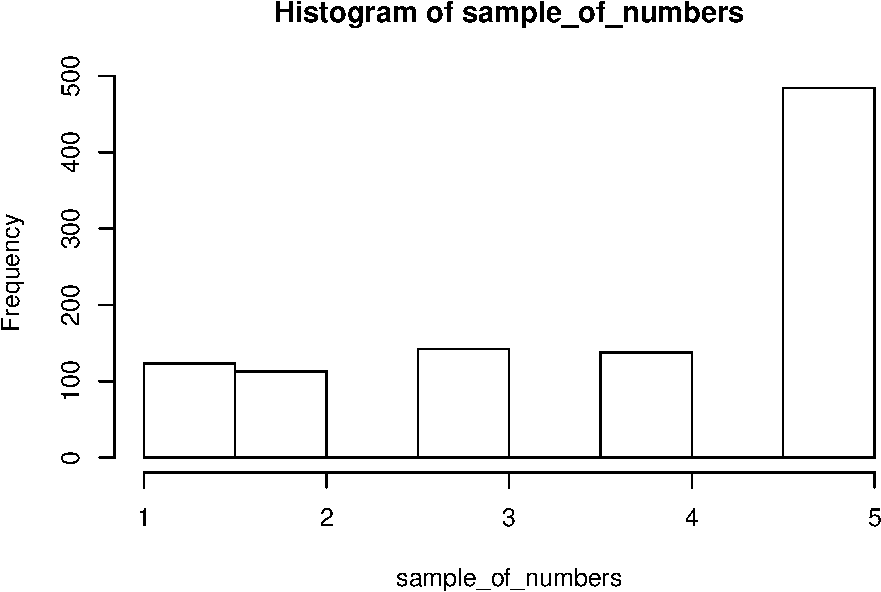
\includegraphics{Programming_Crump_files/figure-latex/unnamed-chunk-68-1.pdf}

\subsubsection{Bar plot}\label{bar-plot}

It's very common to use bars in graphs. We can easily do this by using
\texttt{geom\_bar}, rather than \texttt{geom\_point}. Also, we can plot
bars for the means, and keep showing the dots like this\ldots{}(note
this will be messed up, but I want to show you why).

Also look for these changes.

\begin{enumerate}
\def\labelenumi{\arabic{enumi}.}
\tightlist
\item
  added \texttt{stat="identity"} Necessary for bar plot to show specific
  numbers
\item
  added \texttt{aes(fill=Phase)} Makes each bar a different color,
  depending on which phase it comes from
\end{enumerate}

\begin{Shaded}
\begin{Highlighting}[]
\KeywordTok{ggplot}\NormalTok{(plot_df, }\KeywordTok{aes}\NormalTok{(}\DataTypeTok{x=}\NormalTok{Phase, }\DataTypeTok{y=}\NormalTok{Proportions))+}\StringTok{ }
\StringTok{  }\KeywordTok{geom_point}\NormalTok{()+}
\StringTok{  }\KeywordTok{geom_bar}\NormalTok{(}\DataTypeTok{data=}\NormalTok{mean_df, }\DataTypeTok{stat=}\StringTok{"identity"}\NormalTok{,}\KeywordTok{aes}\NormalTok{(}\DataTypeTok{fill=}\NormalTok{Phase))}
\end{Highlighting}
\end{Shaded}

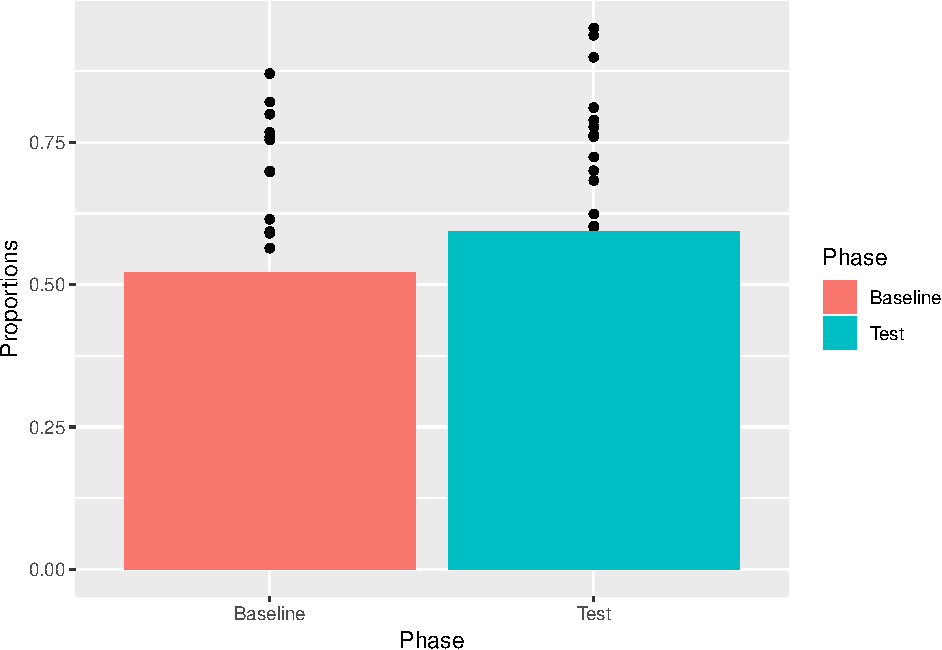
\includegraphics{Programming_Crump_files/figure-latex/unnamed-chunk-69-1.pdf}

Ok, we see the bars and some of the dots, but not all of them. What is
going on? Remember, ggplot2 works in layers. Whatever layer you add
first will be printed first in the graph, whatever layer you add second
will be printed on top of the first. We put the bars on top of the dots.
Let's change the order of the layers so the dot's go on top of the bars.

\begin{Shaded}
\begin{Highlighting}[]
\KeywordTok{ggplot}\NormalTok{(plot_df, }\KeywordTok{aes}\NormalTok{(}\DataTypeTok{x=}\NormalTok{Phase, }\DataTypeTok{y=}\NormalTok{Proportions))+}\StringTok{ }
\StringTok{  }\KeywordTok{geom_bar}\NormalTok{(}\DataTypeTok{data=}\NormalTok{mean_df, }\DataTypeTok{stat=}\StringTok{"identity"}\NormalTok{,}\KeywordTok{aes}\NormalTok{(}\DataTypeTok{fill=}\NormalTok{Phase))+}
\StringTok{  }\KeywordTok{geom_point}\NormalTok{()}
\end{Highlighting}
\end{Shaded}

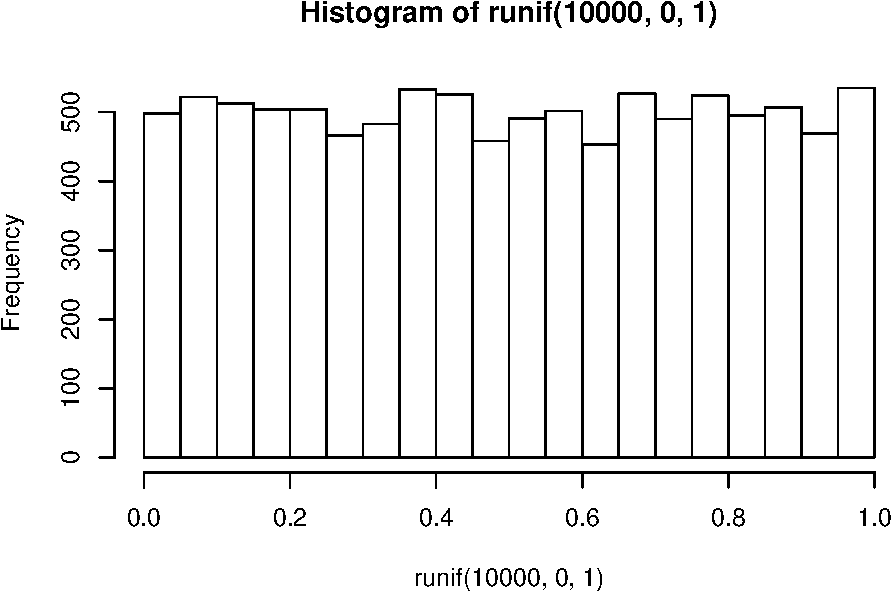
\includegraphics{Programming_Crump_files/figure-latex/unnamed-chunk-70-1.pdf}

\subsubsection{Bar plot with error bars}\label{bar-plot-with-error-bars}

So far we have only plotted the means and individual sample scores.
These are useful, but neither of them give us clear visual information
about our statistical test. Our paired sample t-test suggested that the
mean difference between Baseline and Test was not very likely by chance.
It could have happened, but wouldn't happen very often.

\textbf{Question:} Why would the standard deviation of each mean, or the
standard error of each mean be inappropriate to use in this case?

\textbf{Question:} How would error bars based on the standard error of
the mean differences aid in visual inference about the role of chance in
producing the difference?

Error bars are commonly used as an aid for visual inference. The use of
error bars can be a subtle nuanced issue. This is because there a
different kinds of error bars that can be plotted, and each one supports
different kinds of inference. In general, the error bar is supposed to
represent some aspect of the variability associated with each mean. We
could plot little bars that are +1 or -1 standard deviations of each
mean, or we would do +1 or -1 standard errors of each mean. In the case
of paired samples, neither or these error bars would be appropriate,
they wouldn't reflect the variability associated with mean we are
interested in. In a paired samples t-test, we are interested in the
variability of the mean of the difference scores. Let's calculate the
standard error of the mean (SEM) for the difference scores between
Baseline and Test, and then add error bars to the plot.

\begin{Shaded}
\begin{Highlighting}[]
\NormalTok{difference_scores <-}\StringTok{ }\NormalTok{baseline-test_phase }\CommentTok{#calculate difference scores}
\NormalTok{standard_error <-}\StringTok{ }\KeywordTok{sd}\NormalTok{(difference_scores)/}\KeywordTok{sqrt}\NormalTok{(}\KeywordTok{length}\NormalTok{(difference_scores)) }\CommentTok{#calculate SEM}


\KeywordTok{ggplot}\NormalTok{(plot_df, }\KeywordTok{aes}\NormalTok{(}\DataTypeTok{x=}\NormalTok{Phase, }\DataTypeTok{y=}\NormalTok{Proportions))+}\StringTok{ }
\StringTok{  }\KeywordTok{geom_bar}\NormalTok{(}\DataTypeTok{data=}\NormalTok{mean_df, }\DataTypeTok{stat=}\StringTok{"identity"}\NormalTok{,}\KeywordTok{aes}\NormalTok{(}\DataTypeTok{fill=}\NormalTok{Phase))+}
\StringTok{  }\KeywordTok{geom_errorbar}\NormalTok{(}\DataTypeTok{data=}\NormalTok{mean_df, }\KeywordTok{aes}\NormalTok{(}\DataTypeTok{ymin=}\NormalTok{Proportions-standard_error, }
                                  \DataTypeTok{ymax=}\NormalTok{Proportions+standard_error), }\DataTypeTok{width=}\NormalTok{.}\DecValTok{1}\NormalTok{) +}
\StringTok{  }\KeywordTok{geom_point}\NormalTok{(}\DataTypeTok{alpha=}\NormalTok{.}\DecValTok{25}\NormalTok{)}
\end{Highlighting}
\end{Shaded}

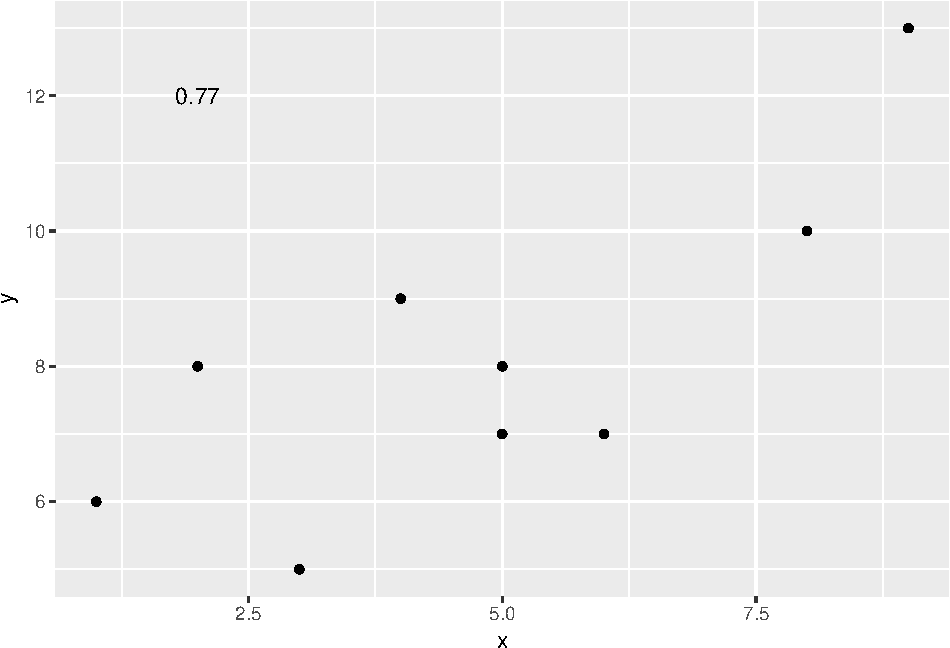
\includegraphics{Programming_Crump_files/figure-latex/unnamed-chunk-71-1.pdf}

\textbf{Question:} What is one reason why these error bars (standard
error of the mean difference between Baseline and Test) are appropriate
to use. What is one reason they are not appropriate to use?

We have done something that is useful for visual inference. From the
textbook, we learned that differences of about 2 standard errors of the
mean are near the point where we would claim that chance is unlikely to
have produced the difference. This is a rough estimate. But, we can see
that the top of the error bar for Baseline is lower than the bottom of
the error bar for Test, resulting in a difference greater than 2
standard error bars. So, based on this graph, we might expect the
difference between conditions to be significant. We can also complain
about what we have done here, we are placing the same error bars from
the meand difference scores onto the means for each condition. In some
sense this is misleading. The error bars are not for the depicted sample
means, they are for the hidden single set of difference scores. To make
this more clear, we will make a bar plot with a single bar only for the
differences scores.

\begin{Shaded}
\begin{Highlighting}[]
\NormalTok{difference_scores <-}\StringTok{ }\NormalTok{test_phase-baseline }\CommentTok{#calculate difference scores}
\NormalTok{standard_error <-}\StringTok{ }\KeywordTok{sd}\NormalTok{(difference_scores)/}\KeywordTok{sqrt}\NormalTok{(}\KeywordTok{length}\NormalTok{(difference_scores)) }\CommentTok{#calculate SEM}
\NormalTok{mean_difference <-}\StringTok{ }\KeywordTok{mean}\NormalTok{(difference_scores)}

\KeywordTok{qplot}\NormalTok{(}\DataTypeTok{x=}\StringTok{"MeanDifference"}\NormalTok{, }\DataTypeTok{y=}\NormalTok{mean_difference)+}
\StringTok{  }\KeywordTok{geom_bar}\NormalTok{(}\DataTypeTok{stat=}\StringTok{"identity"}\NormalTok{, }\DataTypeTok{width=}\NormalTok{.}\DecValTok{5}\NormalTok{, }\DataTypeTok{alpha=}\NormalTok{.}\DecValTok{5}\NormalTok{)+}
\StringTok{  }\KeywordTok{geom_hline}\NormalTok{(}\DataTypeTok{yintercept=}\DecValTok{0}\NormalTok{)+}
\StringTok{  }\KeywordTok{geom_point}\NormalTok{(}\KeywordTok{aes}\NormalTok{(}\DataTypeTok{y=}\NormalTok{difference_scores), }\DataTypeTok{alpha=}\NormalTok{.}\DecValTok{25}\NormalTok{)+}
\StringTok{  }\KeywordTok{geom_errorbar}\NormalTok{(}\KeywordTok{aes}\NormalTok{(}\DataTypeTok{ymin=}\NormalTok{mean_difference-standard_error, }
                                  \DataTypeTok{ymax=}\NormalTok{mean_difference+standard_error), }\DataTypeTok{width=}\NormalTok{.}\DecValTok{1}\NormalTok{)}
\end{Highlighting}
\end{Shaded}

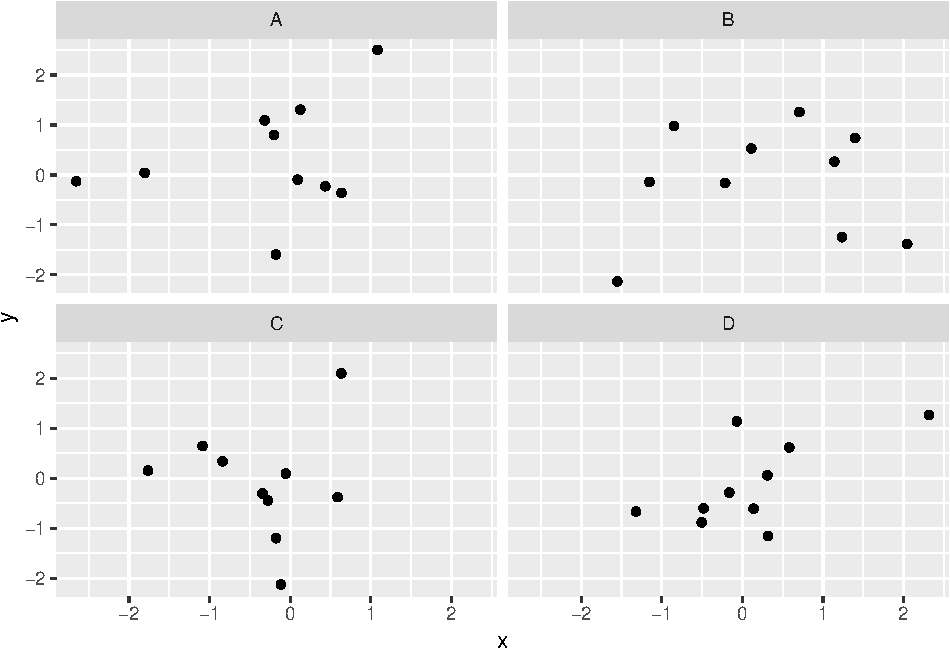
\includegraphics{Programming_Crump_files/figure-latex/unnamed-chunk-72-1.pdf}

\textbf{Question:} Why is is it more appropriate to put the standard
error of the difference on this bar graph? What important aspects of the
original results shown in the previous graph are missing from this
graph?

This plot is very useful too, it gives us some new information. We can
see that the mean difference (test - baseline) was greater than 0. And,
we are plotting the standard error of the mean differences, which are
the error bars that more formally belong to this graph. Still, we are in
a position to make some guesses for visual inference. The lower error
bar represents only 1 SEM. It does not cross 0, but the fact that 1 SEM
does not cross zero isn't important. For SEMs it's usually closer to 2.
We can sort of visually guesstimate that that 2 SEMs would not cross
zero, which would suggest we would obtain a small p-value. We also see
each of the mean difference scores. It's very clear that they are all
over the place. This means that not every infant showed a looking time
preference toward the singer of the familiar song. Finally, this single
bar plot misses something. It doesn't tell us what the values of the
original means were.

\subsubsection{Bar plot with confidence
intervals}\label{bar-plot-with-confidence-intervals}

Confidence intervals are also often used for error bars, rather than the
standard error (or other measure of variance). If we use 95\% confidence
intervals, then our error bars can be even more helpful for visual
inference. Running the \texttt{t.test} function produces confidence
interval estimates, and we can pull them out and use them for error
bars.

\begin{Shaded}
\begin{Highlighting}[]
\NormalTok{t_test_results <-}\StringTok{ }\KeywordTok{t.test}\NormalTok{(difference_scores)}
\NormalTok{lower_interval<-}\StringTok{ }\NormalTok{t_test_results$conf.int[}\DecValTok{1}\NormalTok{]}
\NormalTok{upper_interval<-}\StringTok{ }\NormalTok{t_test_results$conf.int[}\DecValTok{2}\NormalTok{]}

\KeywordTok{qplot}\NormalTok{(}\DataTypeTok{x=}\StringTok{"MeanDifference"}\NormalTok{, }\DataTypeTok{y=}\NormalTok{mean_difference)+}
\StringTok{  }\KeywordTok{geom_bar}\NormalTok{(}\DataTypeTok{stat=}\StringTok{"identity"}\NormalTok{, }\DataTypeTok{width=}\NormalTok{.}\DecValTok{5}\NormalTok{, }\DataTypeTok{alpha=}\NormalTok{.}\DecValTok{5}\NormalTok{)+}
\StringTok{  }\KeywordTok{geom_hline}\NormalTok{(}\DataTypeTok{yintercept=}\DecValTok{0}\NormalTok{)+}
\StringTok{  }\KeywordTok{geom_point}\NormalTok{(}\KeywordTok{aes}\NormalTok{(}\DataTypeTok{y=}\NormalTok{difference_scores), }\DataTypeTok{alpha=}\NormalTok{.}\DecValTok{25}\NormalTok{)+}
\StringTok{  }\KeywordTok{geom_errorbar}\NormalTok{(}\KeywordTok{aes}\NormalTok{(}\DataTypeTok{ymin=}\NormalTok{lower_interval, }
                                  \DataTypeTok{ymax=}\NormalTok{upper_interval), }\DataTypeTok{width=}\NormalTok{.}\DecValTok{1}\NormalTok{)}
\end{Highlighting}
\end{Shaded}

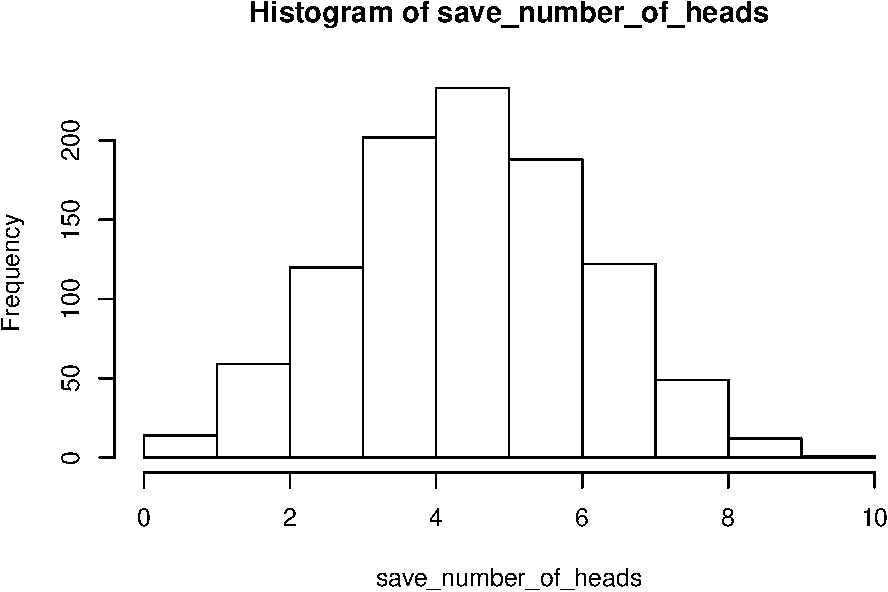
\includegraphics{Programming_Crump_files/figure-latex/unnamed-chunk-73-1.pdf}

Notice that the 95\% confidence intervals around the mean are wider than
the SEM error bars from the previous graph. These new confidence
intervals tell us that 95\% of the time our sample mean will fall
between the two lines. The bottom line is slightly above 0, so we can
now visually see support for our statistical inference that chance was
unlikely to produce the result. If chance was likely to produce the
result, the horizontal line indicating 0, would be well inside the
confidence interval. We can also notice that the mean difference was
just barely different from chance, that lower bar is almost touching 0.

\subsection{Data-simulation}\label{data-simulation}

We can do a little bit of data simulation to get a better feel for this
kind of data. For example, we saw that the dots in our plots were quite
variable. We might wonder about what chance can do in the current
experiment. One way to do this is to estimate the standard deviation of
the looking time proportions. Perhaps the best way to do that would be
to an average of the standard deviation in the baseline and test\_phase
conditions. Then, we could simulate 32 scores from a normal distribution
with mean = .5, and standard deviation equalling our mean standard
deviation. We could calculate the mean of our simulated sample. And, we
could do this many times, say 1000 times. Then, we could look at a
histogram of our means. This will show the range of sample means we
would expect just by chance. This is another way to tell whether the
observed difference in this experiment in the testing phase was close or
not close from being produced by chance. Take a look at the histogram.
What do you think?

\begin{Shaded}
\begin{Highlighting}[]
\NormalTok{sample_sd   <-}\StringTok{ }\NormalTok{(}\KeywordTok{sd}\NormalTok{(baseline)+}\KeywordTok{sd}\NormalTok{(test_phase))/}\DecValTok{2}

\NormalTok{simulated_means <-}\StringTok{ }\KeywordTok{length}\NormalTok{(}\DecValTok{1000}\NormalTok{)}
\NormalTok{for(i in }\DecValTok{1}\NormalTok{:}\DecValTok{1000}\NormalTok{)\{}
 \NormalTok{simulated_means[i] <-}\StringTok{ }\KeywordTok{mean}\NormalTok{(}\KeywordTok{rnorm}\NormalTok{(}\DecValTok{32}\NormalTok{,.}\DecValTok{5}\NormalTok{, sample_sd))}
\NormalTok{\}}

\KeywordTok{hist}\NormalTok{(simulated_means)}
\end{Highlighting}
\end{Shaded}

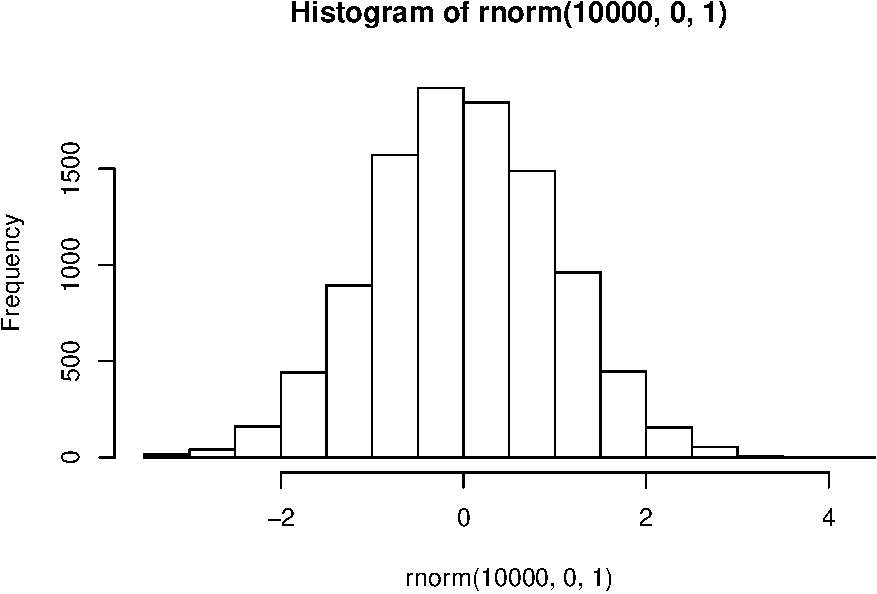
\includegraphics{Programming_Crump_files/figure-latex/unnamed-chunk-74-1.pdf}
\#\#\#\# Simulating the mean differences

We can do the simulation slightly differently to give us a different
look at chance. Above we simulated the sample means from a normal
distibrution centered on .5. The experimental question of interest was
whether the mean difference between the baseline and test\_phase
condition was different. So, we should do a simulation of the difference
scores. First, we estimate the standard deviation of the difference
scores, and then run the simulation with a normal distribution centered
on 0 (an expected mean difference of 0). This shows roughly how often we
might expect mean differences of various sizes to occur. One major
limitation is that we likely had only a rough estimate of the true
standard deviation of these mean differences, after all there were only
32 of them, so we should take this with a grain of salt. Nevertheless,
the pattern in the simulation fits well with the observations in that we
already made from the data.

\begin{Shaded}
\begin{Highlighting}[]
\NormalTok{sample_sd   <-}\StringTok{ }\KeywordTok{sd}\NormalTok{(baseline-test_phase)}

\NormalTok{simulated_mean_difference <-}\StringTok{ }\KeywordTok{length}\NormalTok{(}\DecValTok{1000}\NormalTok{)}
\NormalTok{for(i in }\DecValTok{1}\NormalTok{:}\DecValTok{1000}\NormalTok{)\{}
 \NormalTok{simulated_mean_difference[i] <-}\StringTok{ }\KeywordTok{mean}\NormalTok{(}\KeywordTok{rnorm}\NormalTok{(}\DecValTok{32}\NormalTok{,}\DecValTok{0}\NormalTok{, sample_sd))}
\NormalTok{\}}

\KeywordTok{hist}\NormalTok{(simulated_mean_difference)}
\end{Highlighting}
\end{Shaded}

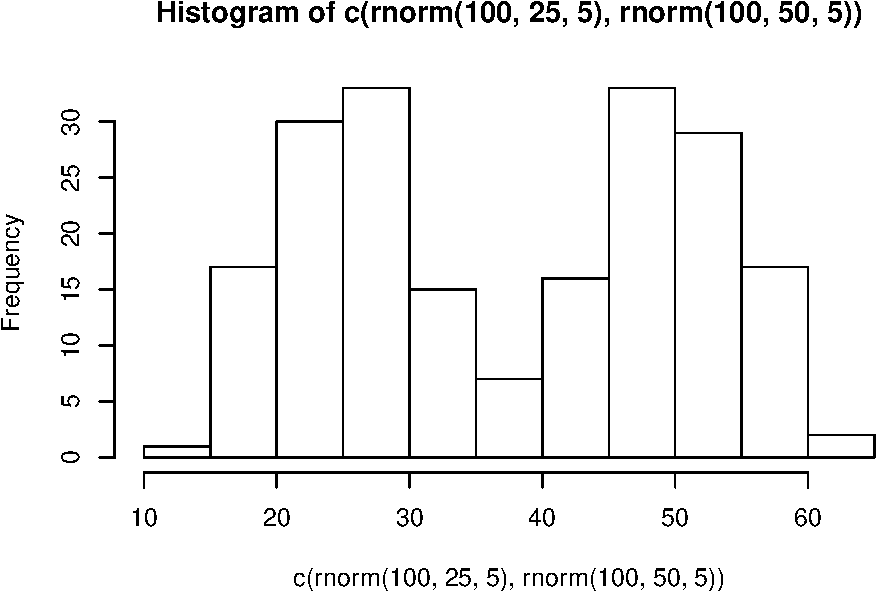
\includegraphics{Programming_Crump_files/figure-latex/unnamed-chunk-75-1.pdf}

\section{Excel}\label{excel-5}

How to do it in Excel

\section{SPSS}\label{spss-5}

How to do it in SPSS

\section{Matlab}\label{matlab-5}

How to do it in Matlab

\chapter{Lab 7: t-test (Independent
Sample)}\label{lab-7-t-test-independent-sample}

This lab is modified and extended from
\href{https://sites.trinity.edu/osl}{Open Stats Labs}. Thanks to Open
Stats Labs (Dr.~Kevin P. McIntyre) for their fantastic work.

\section{Do you come across as smarter when people read what you say or
hear what you
say?}\label{do-you-come-across-as-smarter-when-people-read-what-you-say-or-hear-what-you-say}

\subsection{STUDY DESCRIPTION}\label{study-description-1}

Imagine you were a job candidate trying to pitch your skills to a
potential employer. Would you be more likely to get the job after giving
a short speech describing your skills, or after writing a short speech
and having a potential employer read those words? That was the question
raised by Schroeder and Epley (2015).The authors predicted that a
person's speech (i.e., vocal tone, cadence, and pitch) communicates
information about their intellect better than their written words (even
if they are the same words as in the speech).

To examine this possibility, the authors randomly assigned 39
professional recruiters for Fortune 500 companies to one of two
conditions. In the audio condition, participants listened to audio
recordings of a job candidate's spoken job pitch. In the transcript
condition, participants read a transcription of the job candidate's
pitch. After hearing or reading the pitch, the participants rated the
job candidates on three dimensions: intelligence, competence, and
thoughtfulness. These ratings were then averaged to create a single
measure of the job candidate's intellect, with higher scores indicating
the recruiters rated the candidates as higher in intellect. The
participants also rated their overall impression of the job candidate (a
composite of two items measuring positive and negative impressions).
Finally, the participants indicated how likely they would be to
recommend hiring the job candidate (0 - not at all likely, 10 -
extremely likely).

What happened? Did the recruiters think job applicants were smarter when
they read the transcripts, or when the heard the applicants speak? We
have the data, we can find out.

\section{Lab skills learned}\label{lab-skills-learned-1}

\begin{enumerate}
\def\labelenumi{\arabic{enumi}.}
\tightlist
\item
  Conduct independent samples t-tests
\item
  Generate figures
\item
  Discuss the results and implications
\end{enumerate}

\section{Important Stuff}\label{important-stuff-1}

\begin{itemize}
\tightlist
\item
  citation: Schroeder, J., \& Epley, N. (2015). The sound of intellect:
  Speech reveals a thoughtful mind, increasing a job candidate's appeal.
  Psychological Science, 26, 877-891.
\item
  \href{http://journals.sagepub.com/stoken/default+domain/PhtK6MPtXvkgnYRrnGbA/full}{Link
  to .pdf of article}
\item
  \href{https://drive.google.com/open?id=0Bz-rhZ21ShvOei1MM24xNndnQ00}{Data
  in .csv format}
\item
  \href{https://drive.google.com/open?id=0Bz-rhZ21ShvOVXlDMjEzQU1oY1k}{Data
  in SPSS format}
\end{itemize}

\section{R}\label{r-7}

\subsection{Load the data}\label{load-the-data}

Remember that any line with a \# makes a comment and the code does not
run. Below is how to load the .csv data from the online repository, or
from a local file (you need to change the file path to where the local
file is, if you downloaded it). The data contains all of the measures
and conditions from Experiment 4.

\begin{Shaded}
\begin{Highlighting}[]
\KeywordTok{library}\NormalTok{(data.table)}
\CommentTok{# load from github repo}
\CommentTok{#all_data <- fread("https://raw.githubusercontent.com/CrumpLab/statisticsLab/master/data/SchroederEpley2015data.csv")}

\NormalTok{all_data <-}\StringTok{ }\KeywordTok{fread}\NormalTok{(}\StringTok{"Data/SchroederEpley2015data.csv"}\NormalTok{) }\CommentTok{# load from file on computer}
\end{Highlighting}
\end{Shaded}

\subsection{Inspect data frame}\label{inspect-data-frame}

This will give you a big picture of the data frame. Click the button to
view it in your browser, then take a look to see what is in it.

\begin{Shaded}
\begin{Highlighting}[]
\KeywordTok{library}\NormalTok{(summarytools)}
\KeywordTok{view}\NormalTok{(}\KeywordTok{dfSummary}\NormalTok{(all_data))}
\end{Highlighting}
\end{Shaded}

\subsection{Find the data you need}\label{find-the-data-you-need}

This time the data comes prefiltered for us. The authors ran lots of
experiments, but we only have the data from Experiment 4. This is great,
we don't need to subset the data frame to find all of the data that we
need. But, we do still need to understand what data we want to analyze.
Let's start with identify the column that codes the experimental
conditions for whether or not the evaluator read a transcript or heard
the interview.

\subsubsection{Condition variable}\label{condition-variable}

Lucky for us, the condition variable is called \texttt{CONDITION}! Let's
take a look. We printed it out just by writing down
\texttt{all\_data\$CONDITION}. There 0s and 1s for each condition (audio
vs.~transcript). But which one is which? This isn't clear from the data,
and it isn't clear from the paper, or from the repository. We have to do
some guess work. I went ahead and computed the means for the
Intellect\_rating between each condition, and then compared those to the
graph in the paper for E4. It looks like 1 = audio condition, and 0 =
transcript condition.

\begin{Shaded}
\begin{Highlighting}[]
\NormalTok{all_data$CONDITION}
\end{Highlighting}
\end{Shaded}

\begin{verbatim}
##  [1] 1 1 1 0 0 0 1 0 1 0 0 1 1 0 0 1 1 1 0 0 0 0 0 1 1 1 0 1 1 1 0 0 1 1 0
## [36] 1 0 1 1
\end{verbatim}

\begin{Shaded}
\begin{Highlighting}[]
\KeywordTok{aggregate}\NormalTok{(Intellect_Rating~CONDITION,all_data,mean)}
\end{Highlighting}
\end{Shaded}

\begin{verbatim}
##   CONDITION Intellect_Rating
## 1         0         3.648148
## 2         1         5.634921
\end{verbatim}

Let's use words instead of 0s and 1s to refer to our experimental
conditions. To do this, we will chance the values of 0 and 1, to the
words \texttt{transcript} and \texttt{audio}. We can do this in two
steps. First we convert the CONDITION column to a factor. This will
automatically turn the 0s and 1s into strings (not numbers, text).
Factors have an internal variable for the names of the levels, which
will be 0 and 1. We can simply change the level names to transcript and
audio.

\begin{Shaded}
\begin{Highlighting}[]
\NormalTok{all_data$CONDITION <-}\StringTok{ }\KeywordTok{as.factor}\NormalTok{(all_data$CONDITION)}
\KeywordTok{levels}\NormalTok{(all_data$CONDITION) <-}\StringTok{ }\KeywordTok{c}\NormalTok{(}\StringTok{"transcript"}\NormalTok{,}\StringTok{"audio"}\NormalTok{)}
\end{Highlighting}
\end{Shaded}

Now if you look at the \texttt{all\_data} variable, you will see the
words transcript and audio, where 0s and 1s used to be.

\subsubsection{Dependent Measures}\label{dependent-measures}

Next it's time to find the depende measure columns. The graph from the
paper shows three different measures in each condition. These included
\texttt{Intellect}, \texttt{General\ Impression}, and
\texttt{Hiring\ Likelihood}. Every evaluator (either given a transcript
or audio recording of the interview) gave ratings on a scale of 1 to 10
for each of those concepts. It's not immediately clear which columns in
\texttt{all\_data} correspond to those three measures. There are lots of
different measures that could be the ones they reported. It turns out
the relevant ones are called

\begin{enumerate}
\def\labelenumi{\arabic{enumi}.}
\tightlist
\item
  \texttt{Intellect\_Rating}
\item
  \texttt{Impression\_Rating}
\item
  \texttt{Hire\_Rating}
\end{enumerate}

In this tutorial we are going to walk through doing an independent
samples t-test for the first measure, \texttt{Intellect\_Rating}. You
can follow these same steps to complete the same kind of t-test for the
other two variables.

\subsection{Look at the dependent
variable.}\label{look-at-the-dependent-variable.}

\textbf{Question:} Why do we always want to look at the data?

What is the first thing we do before even considering an inferential
test? Look at the data. Always look at the data. We could make a dot
plot or histogram of the data from the \texttt{Intellect\_ratings}. But,
from our last lab we already learned how to make graphs showing most of
the information we would want to look at. For example, we could make a
bar graph that has the means for each condition (transcript vs.~audio),
standard errors of the mean and the actual scores as little dots. This
would be great to look at it. Not only will it tell us if there are
really weird numbers in the data (who knows maybe the data file is
corrupted, you need to look), it will also give us strong intuitions
about what to expect for the t-test.

We can plot each score as a dot using the \texttt{all\_data} dataframe.
If we want to add on a layer for the sample means, and for the sample
standard errors, we have to compute those and put them in a new
dataframe first. Then we use both dataframes with ggplot to plot all of
the information.

We will use \texttt{dplyr} to quickly get the means and the standard
errors and put them in a new data frame called \texttt{decriptive\_df}.

\begin{Shaded}
\begin{Highlighting}[]
\KeywordTok{library}\NormalTok{(dplyr)}
\KeywordTok{library}\NormalTok{(ggplot2)}

\CommentTok{# get means and SEs}
\NormalTok{descriptive_df <-}\StringTok{ }\NormalTok{all_data %>%}\StringTok{ }
\StringTok{                    }\KeywordTok{group_by}\NormalTok{(CONDITION) %>%}\StringTok{ }
\StringTok{                    }\KeywordTok{summarise}\NormalTok{(}\DataTypeTok{means=} \KeywordTok{mean}\NormalTok{(Intellect_Rating),}
                              \DataTypeTok{SEs =} \KeywordTok{sd}\NormalTok{(Intellect_Rating)/}\KeywordTok{sqrt}\NormalTok{(}\KeywordTok{length}\NormalTok{(Intellect_Rating)))}

\CommentTok{# Make the plot}
\KeywordTok{ggplot}\NormalTok{(descriptive_df, }\KeywordTok{aes}\NormalTok{(}\DataTypeTok{x=}\NormalTok{CONDITION, }\DataTypeTok{y=}\NormalTok{means))+}\StringTok{ }
\StringTok{  }\KeywordTok{geom_bar}\NormalTok{(}\DataTypeTok{stat=}\StringTok{"identity"}\NormalTok{, }\KeywordTok{aes}\NormalTok{(}\DataTypeTok{fill=}\NormalTok{CONDITION))+}\StringTok{ }\CommentTok{# add means}
\StringTok{  }\KeywordTok{geom_errorbar}\NormalTok{(}\KeywordTok{aes}\NormalTok{(}\DataTypeTok{ymin=}\NormalTok{means-SEs,               }\CommentTok{# add error bars}
                    \DataTypeTok{ymax=}\NormalTok{means+SEs), }\DataTypeTok{width=}\NormalTok{.}\DecValTok{1}\NormalTok{) +}
\StringTok{  }\KeywordTok{geom_point}\NormalTok{(}\DataTypeTok{data=}\NormalTok{all_data, }\KeywordTok{aes}\NormalTok{(}\DataTypeTok{x=}\NormalTok{CONDITION, }\DataTypeTok{y=}\NormalTok{Intellect_Rating), }\DataTypeTok{alpha=}\NormalTok{.}\DecValTok{5}\NormalTok{)+}
\StringTok{  }\KeywordTok{geom_point}\NormalTok{(}\DataTypeTok{alpha=}\NormalTok{.}\DecValTok{25}\NormalTok{)+}
\StringTok{  }\KeywordTok{ylab}\NormalTok{(}\StringTok{"Rating"}\NormalTok{)}
\end{Highlighting}
\end{Shaded}

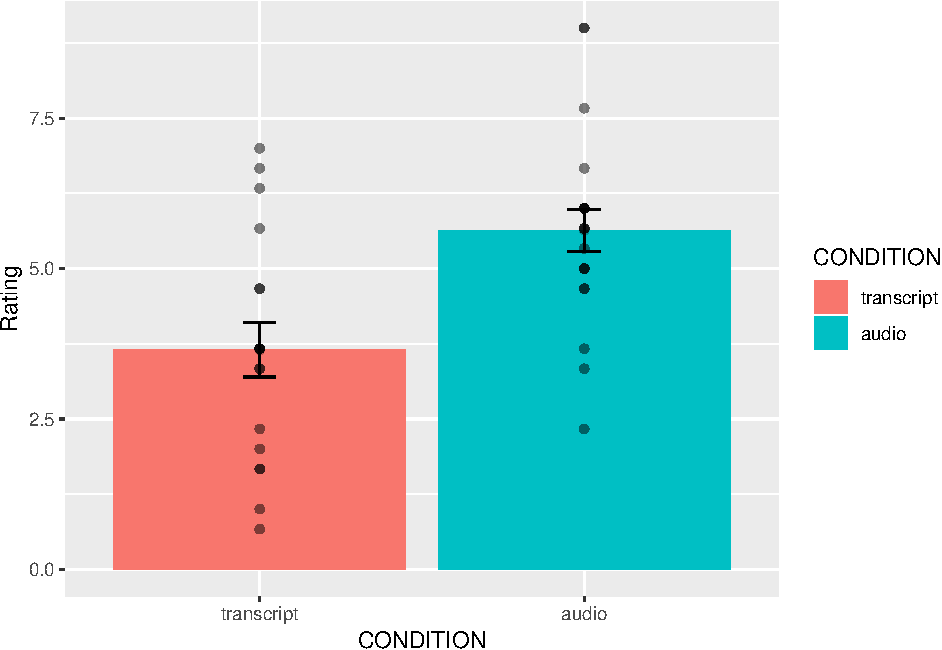
\includegraphics{Programming_Crump_files/figure-latex/unnamed-chunk-80-1.pdf}

This plot is very useful. First, we can see the numbers in our dependent
measure are behaving sensibly. We know that the numbers have to be
between 1-10, because those were the only options in the scale. If we
found numbers bigger or smaller, we would know something was wrong.
Checking for things that are obvsiouly wrong in the data is one reason
why we always look at first. We are checking for obvious errors. There
are other ways to check to, but looking is fast and easy.

\textbf{Question:} Why are the standard errors of each sample an
appropriate thing to use for error bars?

Now that you can see the patterns in the data, you should form an
intuition about how the independent samples t-test will turn out. You
can see how big the error bars (+1/-1 standard error of each sample
man). The t-test will tell us whether the observed difference (or
greater) is likely due to chance. Should we find a big t-value or a
small t-value? Should we find a big p-value or a small t-value. If you
understand how t-values and p-values work, the answer should be very
clear from the graph. You should already know how the t-test will turn
out before you run it. Running it will confirm what you already suspect
to be true.

\subsection{Conduct Independent samples
t-test}\label{conduct-independent-samples-t-test}

\textbf{Question:} Why are we conducting an independent samples t-test,
and not a one-sample or paired samples t-test?

We use the very same \texttt{t.test} function that we used last time to
conduct a t-test. The only difference is that we don't tell the R to use
a paired sample t-test. We leave the \texttt{paired=TRUE} statment out,
and R automatically knows we want to do an independent samples t-test.
Remember to set the \texttt{var.equal=TRUE}, otherwise R will compute a
different version of the t-test.

You can use different syntax to run the t-test. Because our data is
already in a data frame we can use this syntax.

\begin{Shaded}
\begin{Highlighting}[]
\KeywordTok{t.test}\NormalTok{(Intellect_Rating~CONDITION, }\DataTypeTok{data=}\NormalTok{all_data, }\DataTypeTok{var.equal=}\OtherTok{TRUE}\NormalTok{)}
\end{Highlighting}
\end{Shaded}

\begin{verbatim}
## 
##  Two Sample t-test
## 
## data:  Intellect_Rating by CONDITION
## t = -3.5259, df = 37, p-value = 0.001144
## alternative hypothesis: true difference in means is not equal to 0
## 95 percent confidence interval:
##  -3.1284798 -0.8450652
## sample estimates:
## mean in group transcript      mean in group audio 
##                 3.648148                 5.634921
\end{verbatim}

The \texttt{t.test} function also will work on two variables, not in a
data frame. For example, the following does the same thing. But, it's
harder to read, and the means are described in terms of X and Y, not
terms of \texttt{transcript} and \texttt{audio}, like the report above.

\begin{Shaded}
\begin{Highlighting}[]
\KeywordTok{t.test}\NormalTok{(all_data[all_data$CONDITION==}\StringTok{'transcript'}\NormalTok{,]$Intellect_Rating,}
       \NormalTok{all_data[all_data$CONDITION==}\StringTok{'audio'}\NormalTok{,]$Intellect_Rating,}
       \DataTypeTok{var.equal=}\NormalTok{T)}
\end{Highlighting}
\end{Shaded}

\begin{verbatim}
## 
##  Two Sample t-test
## 
## data:  all_data[all_data$CONDITION == "transcript", ]$Intellect_Rating and all_data[all_data$CONDITION == "audio", ]$Intellect_Rating
## t = -3.5259, df = 37, p-value = 0.001144
## alternative hypothesis: true difference in means is not equal to 0
## 95 percent confidence interval:
##  -3.1284798 -0.8450652
## sample estimates:
## mean of x mean of y 
##  3.648148  5.634921
\end{verbatim}

\textbf{Question:} What conclusions do we draw from the t-test? Based on
these results, if you were being evaluated for a job interview, would
you rather have the evaluator read a transcript of your interview or
listen to an audio recording?

So, now we have the t-test. It shows the t-value, the p-value, and the
means for each group. You can double-check with the paper to see if we
found the same results as reported by the authors.

\subsection{Remaining ratings}\label{remaining-ratings}

Now, you should use what you have learned to anlayse the last two
ratings for the dependent variables \texttt{Impression\_Rating}, and
\texttt{Hire\_Rating}. Remember to plot the data for each, and conduct a
t-test for each. Then compare what you found to the original article.
What did you find, and what do the results mean?

\subsection{Reconstructing the graph from the
paper}\label{reconstructing-the-graph-from-the-paper}

The results from Experimen4 4 in the paper plot the means and error bars
(+1 / -1 SEM) for all three dependent measures, for both experimental
conditions. We can do this in ggplot using the data. We will have to
make a couple changes to the dataframe. But, it won't be too hard. What
we need to do is make a fully long form data frame. Remember a long form
data frame has one row per dependent measure.

The \texttt{all\_data} frame is partly long and partly wide. If we are
only interested in one dependent measure, then it is a long data frame
for that measure. For example, example if we are only interested in
plotting \texttt{Intellect\_Rating}, then we already have one
observation of that dependent measure for each row. But, in the other
columns, the dependent measures for \texttt{Impression\_Rating} and
\texttt{Hire\_Rating} are in the same rows.

Before continuing, it is very much worth mentioning that this part of
data analysis happens alot, and it is kind of annoying. I call it the
rubix cube problem, because we need to ``rotate'' and transform the
format of the data to accomplish different kinds of analysis goals. It's
good to be able to know how to do this. This problem occurs all of the
time, can occur for any software package. It's a good thing you are
learning R, because we can do these things easily in R. They are not
often so easy to do without a computer programming language like R. The
worst thing to do is transform the data by hand. That really sucks.
Believe me you don't want to do it. Why? Because you will make mistakes,
and you will mess up the data, then you will mess up your analysis. And,
you won't be able to find your mistakes, and it will take you ages to
correct them. That sucks.

There's more than one way to transform data in R. For example the
\texttt{cast} and \texttt{melt} functions do this kind of thing. You can
look those up. In this example we will not use those functions. Instead
we will show some steps to build the required dataframe one step at a
time.

\begin{Shaded}
\begin{Highlighting}[]
\CommentTok{# repeat CONDITION column three times}

\NormalTok{condition <-}\StringTok{ }\KeywordTok{rep}\NormalTok{(all_data$CONDITION,}\DecValTok{3}\NormalTok{)}

\CommentTok{# make a ratings variable with all three ratings in one variable}

\NormalTok{ratings <-}\StringTok{ }\KeywordTok{c}\NormalTok{(all_data$Intellect_Rating,}
             \NormalTok{all_data$Impression_Rating,}
             \NormalTok{all_data$Hire_Rating)}

\CommentTok{# make a new factor variable with the names of the ratings}
\CommentTok{# need to repeat each level name the appropriate number of times}

\NormalTok{num_to_repeat <-}\StringTok{ }\KeywordTok{length}\NormalTok{(all_data$CONDITION)}

\NormalTok{rating_type <-}\StringTok{ }\KeywordTok{rep}\NormalTok{(}\KeywordTok{c}\NormalTok{(}\StringTok{"Intellect"}\NormalTok{,}\StringTok{"Impression"}\NormalTok{,}\StringTok{"Hire"}\NormalTok{),num_to_repeat)}

\CommentTok{# put the new variables into a data frame}

\NormalTok{plot_all <-}\StringTok{ }\KeywordTok{data.frame}\NormalTok{(condition,rating_type,ratings)}

\CommentTok{# Get the means and standard errors for each rating by condition}

\NormalTok{descriptive_all <-}\StringTok{ }\NormalTok{plot_all %>%}\StringTok{ }
\StringTok{                    }\KeywordTok{group_by}\NormalTok{(condition,rating_type) %>%}\StringTok{ }
\StringTok{                    }\KeywordTok{summarise}\NormalTok{(}\DataTypeTok{means=} \KeywordTok{mean}\NormalTok{(ratings),}
                              \DataTypeTok{SEs =} \KeywordTok{sd}\NormalTok{(ratings)/}\KeywordTok{sqrt}\NormalTok{(}\KeywordTok{length}\NormalTok{(ratings)))}

\CommentTok{# Make the plot}

\KeywordTok{ggplot}\NormalTok{(descriptive_all, }\KeywordTok{aes}\NormalTok{(}\DataTypeTok{x=}\NormalTok{rating_type, }\DataTypeTok{y=}\NormalTok{means, }\DataTypeTok{group=}\NormalTok{condition))+}\StringTok{ }
\StringTok{  }\KeywordTok{geom_bar}\NormalTok{(}\DataTypeTok{stat=}\StringTok{"identity"}\NormalTok{, }\KeywordTok{aes}\NormalTok{(}\DataTypeTok{fill=}\NormalTok{condition), }\DataTypeTok{position=}\StringTok{'dodge'}\NormalTok{)+}\StringTok{ }
\StringTok{  }\KeywordTok{geom_errorbar}\NormalTok{(}\KeywordTok{aes}\NormalTok{(}\DataTypeTok{ymin=}\NormalTok{means-SEs,               }
                    \DataTypeTok{ymax=}\NormalTok{means+SEs), }
                \DataTypeTok{width=}\NormalTok{.}\DecValTok{1}\NormalTok{, }
                \DataTypeTok{position =} \KeywordTok{position_dodge}\NormalTok{(}\DataTypeTok{width=}\NormalTok{.}\DecValTok{9}\NormalTok{)) +}
\StringTok{  }\KeywordTok{geom_point}\NormalTok{(}\DataTypeTok{data=}\NormalTok{plot_all, }\KeywordTok{aes}\NormalTok{(}\DataTypeTok{x=}\NormalTok{rating_type, }
                                \DataTypeTok{y=}\NormalTok{ratings, }
                                \DataTypeTok{group=}\NormalTok{condition), }
             \DataTypeTok{alpha=}\NormalTok{.}\DecValTok{25}\NormalTok{, }
             \DataTypeTok{position =} \KeywordTok{position_dodge}\NormalTok{(}\DataTypeTok{width=}\NormalTok{.}\DecValTok{9}\NormalTok{))+}
\StringTok{  }\KeywordTok{geom_point}\NormalTok{(}\DataTypeTok{alpha=}\NormalTok{.}\DecValTok{25}\NormalTok{)+}
\StringTok{  }\KeywordTok{ylab}\NormalTok{(}\StringTok{"Rating"}\NormalTok{)}
\end{Highlighting}
\end{Shaded}

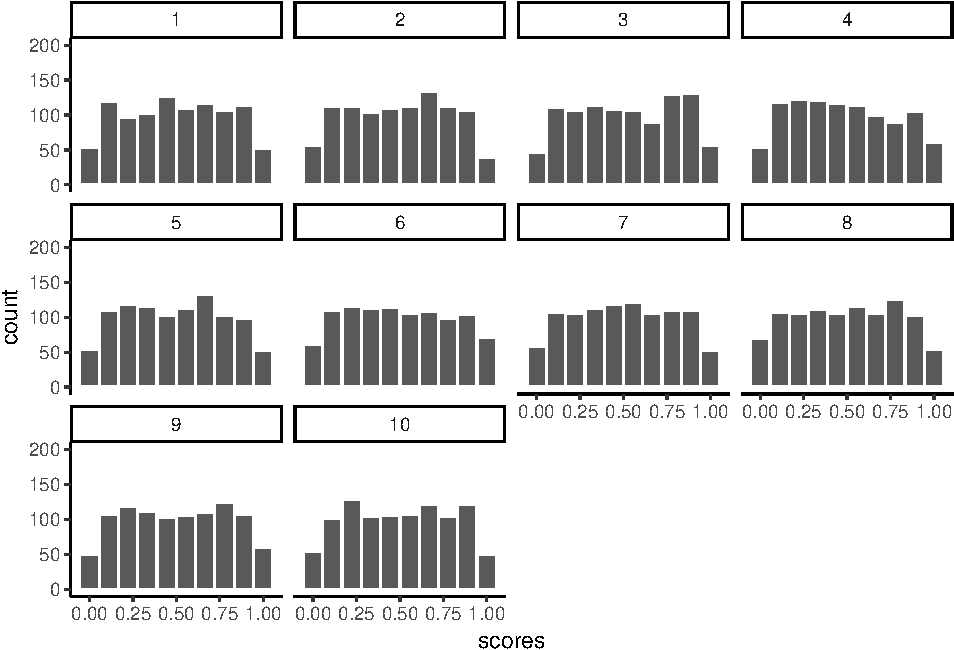
\includegraphics{Programming_Crump_files/figure-latex/unnamed-chunk-83-1.pdf}

Well, we didn't make the exact graph. We have the bars, the error bars,
and we added the individual scores because they are useful to look at.
Otherwise, it's the same graph (except the the ordering of bars is
determined alphabetically here. We change that in ggplot, but we won't
do that today.)

\section{Excel}\label{excel-6}

How to do it in Excel

\section{SPSS}\label{spss-6}

How to do it in SPSS

\section{Matlab}\label{matlab-6}

How to do it in Matlab

\chapter{Lab 8: One-way ANOVA}\label{lab-8-one-way-anova}

This lab is modified and extended from
\href{https://sites.trinity.edu/osl}{Open Stats Labs}. Thanks to Open
Stats Labs (Dr.~Kevin P. McIntyre) for their fantastic work.

\section{How to not think about bad memories by playing
Tetris}\label{how-to-not-think-about-bad-memories-by-playing-tetris}

This lab activity uses the open data from Experiment 2 of James et al.
(2015) to teach one-way ANOVA with planned comparisons. Results of the
activity provided below should exactly reproduce the results described
in the paper.

\subsection{STUDY DESCRIPTION}\label{study-description-2}

Following traumatic experiences, some people have flashbacks, which are
also called ``intrusive memories''" and are characterized by involuntary
images of aspects of the traumatic event. Although people often try to
simply forget traumatic memories, this approach is not very effective.
Instead, previous research suggests that a better approach may be to try
to change aspects of the memory after it is formed. For example, some
research shows that traumatic memories can be altered and weakened to
the point that they are no longer intrusive.

Because intrusive memories of trauma are often visual in nature, James
and colleagues (2015) sought to explore whether completing a
visuospatial task (e.g., Tetris) after a memory was formed would
interfere with the storage of that memory, and thereby reduce the
frequency of subsequent intrusions. They hypothesized that only
participants who complete a visuo-spatial task after reactivation of the
traumatic memories would experience a reduction in intrusive memories.
In comparison, simply completing a visuo-spatial task (without
reactivation) or reactivation (without a visuo-spatial task), would not
reduce the occurrence intrusive memories.

In other words, if you play Tetris shortly after you were remembering
bad memories, playing Tetris might weaken those memories, which could
cause you experience those kinds of intrusive memories less often in the
future.

\subsection{Study Methods}\label{study-methods}

To test their hypothesis, the authors conducted an experiment ( N = 72,
n = 18 per condition). The procedure is summarized as follows:

\textbf{Trauma Film}: All participants viewed a series of video clips of
graphic violence (e.g., a person getting hit by a van while using his
phone as he crosses the road) as a way to create memories that should
become intrusive memories. Participants then went home and recorded the
number of intrusive memories they experienced over the next 24 hours.
Because this is before the experimental manipulations, all groups were
predicted to have an equal occurrence of intrusive memories during the
first 24-hours (called Day 0).

\textbf{Experimental Task}: After this 24-hour period, the participants
returned to the lab and completed the experimental task. The
experimenters randomly assigned participants to ONE of the following
conditions:

\begin{enumerate}
\def\labelenumi{\arabic{enumi}.}
\tightlist
\item
  No-task control: These participants completed a 10-minute music filler
  task.
\item
  Reactivation + Tetris: These participants were shown a series of
  images from the trauma film to reactivate the traumatic memories
  (i.e., reactivation task). After a 10-minute music filler task,
  participants played the video game Tetris for 12 minutes.
\item
  Tetris Only: These participants played Tetris for 12 minutes, but did
  not complete the reactivation task.
\item
  Reactivation Only: These participants completed the reactivation task,
  but did not play Tetris.
\end{enumerate}

\textbf{Intrusive Memories}: All participants were asked to record the
number of intrusive memories that they experienced over the next seven
days (Days 1 to 7).

After the seven days had passed, participants completed an
Intrusion-Provocation Task, in which they were shown blurred images from
the trauma film and asked to indicate whether the blurred image
triggered an intrusive memory.

\section{Lab Skills Learned}\label{lab-skills-learned-2}

\section{Important Stuff}\label{important-stuff-2}

\begin{itemize}
\tightlist
\item
  citation: James, E. L., Bonsall, M. B., Hoppitt, L., Tunbridge, E. M.,
  Geddes, J. R., Milton, A. L., \& Holmes, E. A. (2015). Computer game
  play reduces intrusive memories of experimental trauma via
  re-consolidation-update mechanisms. Psychological Science, 26,
  1201-1215.
\item
  \href{http://journals.sagepub.com/stoken/default+domain/hQ2W4fbPrZVJ7eyNJaqu/full}{Link
  to .pdf of article}
\item
  \href{https://drive.google.com/open?id=0Bz-rhZ21ShvOM1cxWUpUNlQ0UlE}{Data
  in .csv format}
\item
  \href{https://drive.google.com/file/d/0Bz-rhZ21ShvOZ1lvQ0dQekZGWU0/view?usp=sharing}{Data
  in SPSS format}
\end{itemize}

\section{R}\label{r-8}

\subsection{Load the data}\label{load-the-data-1}

Remember that any line with a \# makes a comment and the code does not
run. Below is how to load the .csv data from the online repository, or
from a local file (you need to change the file path to where the local
file is, if you downloaded it). The data contains all of the measures
and conditions from Experiment 2 in the paper.

\begin{Shaded}
\begin{Highlighting}[]
\KeywordTok{library}\NormalTok{(data.table)}
\CommentTok{#fread("https://raw.githubusercontent.com/CrumpLab/statisticsLab/master/data/Jamesetal2015Experiment2.csv")}
\NormalTok{all_data <-}\StringTok{ }\KeywordTok{fread}\NormalTok{(}\StringTok{"data/Jamesetal2015Experiment2.csv"}\NormalTok{)}
\end{Highlighting}
\end{Shaded}

\subsection{Inspect the dataframe}\label{inspect-the-dataframe}

This will give you a big picture of the data frame. Click the button to
view it in your browser, then take a look to see what is in it.

\begin{Shaded}
\begin{Highlighting}[]
\KeywordTok{library}\NormalTok{(summarytools)}
\KeywordTok{view}\NormalTok{(}\KeywordTok{dfSummary}\NormalTok{(all_data))}
\end{Highlighting}
\end{Shaded}

\subsection{Get the data you need}\label{get-the-data-you-need}

Again we have only the data from Experiment 2, so we don't need to get
rid of any rows of the data. But we do need look at the columns to see
how the independent variable and dependent variables were coded.

\subsubsection{The independent variable}\label{the-independent-variable}

There was one important independent variable, and it had four levels.
The first column in the data frame is called condition, and it has four
levels. The levels are 1, 2, 3, and 4 in the data-frame. These will
correspond to the four levels in shown in figure:

\begin{itemize}
\tightlist
\item
  No-task control
\item
  Reactivation Plus Tetris
\item
  Tetris only
\item
  Reactivation only
\end{itemize}

Each of these refer to what subjects did after they watched the
traumatic film. But, which of these correspond to the numbers 1 to 4 in
the data-frame? It turns out the are in the right order, and 1 to 4
refer to:

\begin{enumerate}
\def\labelenumi{\arabic{enumi}.}
\tightlist
\item
  No-task control
\item
  Reactivation Plus Tetris
\item
  Tetris only
\item
  Reactivation only
\end{enumerate}

Let's do ourselves a favor and rename the levels of the
\texttt{Condition} column with words so we know what they refer to.
First, convert the \texttt{Condition} column to a factor, then rename
the levels. Then.

\begin{Shaded}
\begin{Highlighting}[]
\NormalTok{all_data$Condition <-}\StringTok{ }\KeywordTok{as.factor}\NormalTok{(all_data$Condition)}
\KeywordTok{levels}\NormalTok{(all_data$Condition) <-}\StringTok{ }\KeywordTok{c}\NormalTok{(}\StringTok{"Control"}\NormalTok{,}
                                \StringTok{"Reactivation+Tetris"}\NormalTok{, }
                                \StringTok{"Tetris_only"}\NormalTok{,}
                                \StringTok{"Reactivation_only"}\NormalTok{)}
\end{Highlighting}
\end{Shaded}

\subsubsection{The dependent variable}\label{the-dependent-variable}

The authors showed two figures, one where they analysed intrusive memory
frequency as the mean for the week, and the other where the used
intrusive memory frequency on Day 7. In this tutorial, we will do the
steps to run an ANOVA on the mean for the week data, and you will do
follow these steps to run another ANOVA on the Day 7 data.

The mean for the week data for each subject is apparently coded in the
column \texttt{Days\_One\_to\_Seven\_Number\_of\_Intrusions}.

\subsection{Look at the data}\label{look-at-the-data-1}

Remember before we do any analysis, we always want to ``look'' at the
data. This first pass let's us know if the data ``look right''. For
example, the data file could be messed up and maybe there aren't any
numbers there, or maybe the numbers are just too weird.

In the last two labs, we saw how to show all the data we are interested
in looking at in one go. We can do the same things here. For example, in
one little piece of code, we can display the means in each condition,
the standard errors of the mean, and the individual scores for each
subject in each condition. This is a lot to look at, but it's everything
we want to look at for starters all in the same place. Looking at the
data this way will also give us intuitions about what our ANOVA will
tell us before we run the ANOVA. This is helpful for determining whether
the results of your ANOVA are accurate or not. Let's do it\ldots{}also
notice that the code is very similar to what we did for the independent
t-test. In fact, all I did was copy and paste that code right here, and
edited it a little bit. This is really fast, and shows the efficiency of
doing things this way.

\begin{Shaded}
\begin{Highlighting}[]
\KeywordTok{library}\NormalTok{(dplyr)}

\KeywordTok{library}\NormalTok{(ggplot2)}

\CommentTok{# get means and SEs}
\NormalTok{descriptive_df <-}\StringTok{ }\NormalTok{all_data %>%}\StringTok{ }
\StringTok{                    }\KeywordTok{group_by}\NormalTok{(Condition) %>%}\StringTok{ }
\StringTok{                    }\KeywordTok{summarise}\NormalTok{(}\DataTypeTok{means=} \KeywordTok{mean}\NormalTok{(Days_One_to_Seven_Number_of_Intrusions),}
                              \DataTypeTok{SEs =} \KeywordTok{sd}\NormalTok{(Days_One_to_Seven_Number_of_Intrusions)/}\KeywordTok{sqrt}\NormalTok{(}\KeywordTok{length}\NormalTok{(Days_One_to_Seven_Number_of_Intrusions)))}

\CommentTok{# Make the plot}
\KeywordTok{ggplot}\NormalTok{(descriptive_df, }\KeywordTok{aes}\NormalTok{(}\DataTypeTok{x=}\NormalTok{Condition, }\DataTypeTok{y=}\NormalTok{means))+}\StringTok{ }
\StringTok{  }\KeywordTok{geom_bar}\NormalTok{(}\DataTypeTok{stat=}\StringTok{"identity"}\NormalTok{, }\KeywordTok{aes}\NormalTok{(}\DataTypeTok{fill=}\NormalTok{Condition))+}\StringTok{ }\CommentTok{# add means}
\StringTok{  }\KeywordTok{geom_errorbar}\NormalTok{(}\KeywordTok{aes}\NormalTok{(}\DataTypeTok{ymin=}\NormalTok{means-SEs,               }\CommentTok{# add error bars}
                    \DataTypeTok{ymax=}\NormalTok{means+SEs), }\DataTypeTok{width=}\NormalTok{.}\DecValTok{1}\NormalTok{) +}
\StringTok{  }\KeywordTok{geom_point}\NormalTok{(}\DataTypeTok{data=}\NormalTok{all_data, }\KeywordTok{aes}\NormalTok{(}\DataTypeTok{x=}\NormalTok{Condition, }\DataTypeTok{y=}\NormalTok{Days_One_to_Seven_Number_of_Intrusions), }\DataTypeTok{alpha=}\NormalTok{.}\DecValTok{5}\NormalTok{)+}
\StringTok{  }\KeywordTok{geom_point}\NormalTok{(}\DataTypeTok{alpha=}\NormalTok{.}\DecValTok{25}\NormalTok{)+}
\StringTok{  }\KeywordTok{ylab}\NormalTok{(}\StringTok{"Intrusive Memories (Mean for Week)"}\NormalTok{)}
\end{Highlighting}
\end{Shaded}

\includegraphics{Programming_Crump_files/figure-latex/unnamed-chunk-87-1.pdf}

There we have it. A nice graph showing us everything. We can see there
was a lot of differences at the level of individual subjects. Some
subjects had a mean of 15 intrusive memories for the week. Some had 0.
Lots of differences.

And, to be completely honest, this data seems a bit weird to me. It
might not be weird, but it might be. The wording in the manuscript is
that this data is the mean frequency of intrusive memories over the
week. For the people who had 15, this means that every day they had on
average 15 intrusive memories. Some people had on average 0 per day.
This could be the data. But, it also seems like the data might just be
frequency counts and not means at all. For example, the data could be
that some people had a total of 15 intrusive over the week. The data
might make more sense if these were frequency counts. Otherwise the
differences between people are truly very large. For example the person
who had an average of 15 intrusive memories per week, must have had 15*7
= 105 intrusive memories, which is a lot more than zero. In any case,
this kind of wondering about the data is what happens when you start to
notice how numbers work. It's useful develop your data sense.

Let's move on to the ANOVA. By looking at the above graph do you have an
intuition about what the ANOVA will tell us? I do, it should easily tell
us that we are going to get an F-value that is bigger than one, and a
p-value that is probably smaller than .05? How do I know this? I looked
at the error bars, which represent the standard errors of the mean. If
we look across conditions we can see that that the error bars don't
always overlap. This suggests there are differences in the data that
don't happen very often by chance. So, we expect a smallish p-value. Why
do you think I expect the F-value to be greater than 1? If you can
answer this question with a justification and explanation of how F
works, pat yourself on the back!

\subsection{Conduct the ANOVA}\label{conduct-the-anova}

Conducting an ANOVA in R is pretty easy. It's one line of code, just
like the t-test.

It's worth knowing that there are a few different packages out there to
do an ANOVA, for example Mike Lawrence's \texttt{ezANOVA} package is
pretty popular.

For this tutorial we'll show you how to run the ANOVA using the
\texttt{aov} function from base R (comes pre-installed). This is pretty
``easy'' too. I put easy in quotes because the first time I saw this, it
was not easy for me. Here's a brief digression for me to tell you that I
feel your pain. I was first introduced to R by Patrick Bennett (a
professor at McMaster University, where I attended graduate school).
Pat, like I am doing know, forced us to use R in his statistics class. I
remember having zero clue about so many things, and was often very
frustrated. So, I imagine some of you are quite frustrated too. I was
luck, like some of you, to have had some previous experience with other
programming languages, so I was familiar with what R might be doing.
What I was most frustrated with, was learning how to tell R what to do.
In other words, I didn't know how to write the commands properly. I
didn't understand what we call the \textbf{syntax} of R.

This was back many years ago now, well before there was so many helpful
examples on Google with working code, showing you how the syntax works.
All we had was the R help files, which were a total mystery to me. If
you want to see the help file for \texttt{aov}, just type
\texttt{?aov()} into the console, and press enter. You will see an
``explanation'' of how the \texttt{aov} function is supposed to work.
You can use the same trick for any R function, like this
\texttt{?name\_of\_function()}. To be clear, you have to replace the
letters \texttt{name\_of\_function}, with the name of the function. Some
of you think that might be super obvious, but that is the kind of thing
I did not think was obvious. So, when I read the help file for how to
use the \texttt{aov} function, that is to learn what to put where, I
didn't feel like it was showing me what I needed to do. Usually, at the
bottom of the help file, there are some examples, and these are helpful,
but sometimes they are missing the example you need, and you are
expected to generalize your knowledge of how \texttt{aov} works, to make
it work for your problem. This is a catch-22 because if you don't know
how it works, you can't generalize. IMO, you need a lot of examples of
things that work.

So, with that digression, I'm going to explain the syntax for the aov
function. It looks like this:

\texttt{aov(DV\ \textasciitilde{}\ IV,\ dataframe)}

That probably looks really foreign. Let me explain. First you need write
\texttt{aov()}. \texttt{aov} is the name of the function, followed by
the brackets. The brackets are a sandwich. Sandwiches have a top and a
bottom, and they enclose the things you put in the sandwich. We then put
things inside the \texttt{()}, in specific ways to make the \texttt{aov}
sandwich. The \texttt{DV} stands for the name of the dependent variable
in the data frame. For us, this will be
\texttt{Days\_One\_to\_Seven\_Number\_of\_Intrusions}. So, when we add
that, our function will look like:

\texttt{aov(Days\_One\_to\_Seven\_Number\_of\_Intrusions\ \textasciitilde{}\ IV,\ dataframe)}

Next, the \texttt{\textasciitilde{}} (tilda) stands for the word `by'.
We are saying we want to analyse the Dependent variable \textbf{by} the
conditions of the independent variable.

The \texttt{IV} stands for the name of the column that is your
independent variable. Our's is called \texttt{Condition}. Adding that
in, our formula looks like:

\texttt{aov(Days\_One\_to\_Seven\_Number\_of\_Intrusions\ \textasciitilde{}\ Condition,\ dataframe)}

Finally, the last part is the name of the data-frame we are using. The
\texttt{aov} function only works on long-form data, where each score on
the dependent variable has it's own row. Our's is already set up this
way! The name of our data-frame is \texttt{all\_data}. We add that in,
and it looks like:

\texttt{aov(Days\_One\_to\_Seven\_Number\_of\_Intrusions\ \textasciitilde{}\ Condition,\ all\_data)}

In English, this means, do an ANOVA on the dependent variable as a
function of the independent variable, and use the data in my data frame.

This is it for now. The \texttt{aov} function is very flexible because
you can define different kinds of formulas (the
\texttt{DV\ \textasciitilde{}\ IV} part). We'll see other examples in
later chapters. For now, this is all we need. Also, what's cool, is that
this will work for any single IV with any number of levels (conditions)
2 or greater. Fun. Let's see it in action.

\begin{Shaded}
\begin{Highlighting}[]
\KeywordTok{aov}\NormalTok{(Days_One_to_Seven_Number_of_Intrusions ~}\StringTok{ }\NormalTok{Condition, all_data)}
\end{Highlighting}
\end{Shaded}

\begin{verbatim}
## Call:
##    aov(formula = Days_One_to_Seven_Number_of_Intrusions ~ Condition, 
##     data = all_data)
## 
## Terms:
##                 Condition Residuals
## Sum of Squares   114.8194  685.8333
## Deg. of Freedom         3        68
## 
## Residual standard error: 3.175812
## Estimated effects may be unbalanced
\end{verbatim}

What is this garbage? I don't see an ANOVA table, what is this? You are
seeing the raw print out of the aov function. Clearly, this is not
helpful, it's not what we want to see.

Fortunately, R comes with another function called \texttt{summary}. What
it does is summarize the results of functions like \texttt{aov}, and
prints them out in a nicer way. Let's see the summary function do it's
thing:

\begin{Shaded}
\begin{Highlighting}[]
\KeywordTok{summary}\NormalTok{(}\KeywordTok{aov}\NormalTok{(Days_One_to_Seven_Number_of_Intrusions ~}\StringTok{ }\NormalTok{Condition, all_data))}
\end{Highlighting}
\end{Shaded}

\begin{verbatim}
##             Df Sum Sq Mean Sq F value Pr(>F)  
## Condition    3  114.8   38.27   3.795 0.0141 *
## Residuals   68  685.8   10.09                 
## ---
## Signif. codes:  0 '***' 0.001 '**' 0.01 '*' 0.05 '.' 0.1 ' ' 1
\end{verbatim}

Alright, now we have an ANOVA table we can look at. However, it still
looks ugly, at least to me. When you are working inside an R Markdown
document, you have some more options to make it look nice. We can use
the \texttt{kable} and \texttt{xtable} function together, like this.

\begin{Shaded}
\begin{Highlighting}[]
\KeywordTok{library}\NormalTok{(xtable)}
\NormalTok{aov_out<-}\KeywordTok{aov}\NormalTok{(Days_One_to_Seven_Number_of_Intrusions ~}\StringTok{ }\NormalTok{Condition, all_data)}
\NormalTok{summary_out<-}\KeywordTok{summary}\NormalTok{(aov_out)}

\NormalTok{knitr::}\KeywordTok{kable}\NormalTok{(}\KeywordTok{xtable}\NormalTok{(summary_out))}
\end{Highlighting}
\end{Shaded}

\begin{tabular}{l|r|r|r|r|r}
\hline
  & Df & Sum Sq & Mean Sq & F value & Pr(>F)\\
\hline
Condition & 3 & 114.8194 & 38.27315 & 3.794762 & 0.0140858\\
\hline
Residuals & 68 & 685.8333 & 10.08578 & NA & NA\\
\hline
\end{tabular}

Now we see a nicer print out. Especially if we \texttt{knit} the
document into a webpage.

\subsection{Reporting the ANOVA
results}\label{reporting-the-anova-results}

Refer tot the textbook on ANOVAs for a deeper discussion of all the
things in the ANOVA table. We'll remind about some of those things here.

First, let's look at how we might report the results. There are three
very important parts to this.

\begin{enumerate}
\def\labelenumi{\arabic{enumi}.}
\tightlist
\item
  Saying what test you did to what data
\item
  Reporting the inferential statistics
\item
  Reporting the pattern in the means
\end{enumerate}

Here is part 1, we need to say what data we used, and what kind of test
we used on that data:

\begin{quote}
We submitted the mean intrusive memories for the week from each subject
in each condition to a one-factor betwee-subjects ANOVA, with
Intervention type (No-task control, Reactivation Plus tetris, Tetris
only, Reactivation only) as the sole independent variable.
\end{quote}

Part 2 is saying what the results of the test were. Specifically, we
report the values from the inferential test (see the textbook for why
these values). Also, you should be able to answer this question: why do
we report the values that we do?

\begin{quote}
We found a main effect of Intervention type, F(3, 68) = 3.79, MSE =
10.09, p = 0.014.
\end{quote}

Part 3 is saying what the pattern was in the means. Remember, that in
the ANOVA, a significant effect refers to the global variation among the
means. In other words, we can say that there are some differences
between the means, but we can't specifically say which pairs of means
are different, or which groups of means are different from one another.
How can we report this, where are the means? In fact, we already found
them when we plotted the data earlier. So, we can copy paste that code,
and print out the means, rather than the figure:

\begin{Shaded}
\begin{Highlighting}[]
\CommentTok{# get means and SEs}
\NormalTok{descriptive_df <-}\StringTok{ }\NormalTok{all_data %>%}\StringTok{ }
\StringTok{                    }\KeywordTok{group_by}\NormalTok{(Condition) %>%}\StringTok{ }
\StringTok{                    }\KeywordTok{summarise}\NormalTok{(}\DataTypeTok{means=} \KeywordTok{mean}\NormalTok{(Days_One_to_Seven_Number_of_Intrusions),}
                              \DataTypeTok{SEs =} \KeywordTok{sd}\NormalTok{(Days_One_to_Seven_Number_of_Intrusions)/}\KeywordTok{sqrt}\NormalTok{(}\KeywordTok{length}\NormalTok{(Days_One_to_Seven_Number_of_Intrusions)))}

\NormalTok{knitr::}\KeywordTok{kable}\NormalTok{(descriptive_df)}
\end{Highlighting}
\end{Shaded}

\begin{tabular}{l|r|r}
\hline
Condition & means & SEs\\
\hline
Control & 5.111111 & 0.9963623\\
\hline
Reactivation+Tetris & 1.888889 & 0.4113495\\
\hline
Tetris\_only & 3.888889 & 0.6806806\\
\hline
Reactivation\_only & 4.833333 & 0.7848650\\
\hline
\end{tabular}

No we have to use a sentence to describe these means.

\begin{quote}
Refer to table 1 for the means and standard errors of the mean in each
condition
\end{quote}

or,

\begin{quote}
Mean intrusive memories per week were 5.11 (SE = .99); 1.89 (SE = .41);
3.89 (SE = .68); and 4.83 (SE= .78), in the Control, Reaction plus
Tetris, Tetris Only, and Reactivation only conditions, respectively
\end{quote}

Ugh, what a mouthful. Be mindful of how you write results. The above is
not helpful because you see a list of numbers, and then a list of
conditions, and the reader has to do a lot of work to keep everything
straight. I like the table option.

I also like this other kind of option:

\begin{quote}
Mean intrusive memories were significantly different between the Control
(M = 5.11, SE = .99), Reactivation plus Tetris (M = 3.89, SE = .68),
Tetris only (M= 3.89, SE = .68), and Reactivation only (M = 4.83, .78)
conditions.
\end{quote}

That's a little bit better. Let's put it all in one place to see what it
look like:

\begin{quote}
We submitted the mean intrusive memories for the week from each subject
in each condition to a one-factor betwee-subjects ANOVA, with
Intervention type (No-task control, Reactivation Plus tetris, Tetris
only, Reactivation only) as the sole independent variable. We found a
main effect of Intervention type, F(3, 68) = 3.79, MSE = 10.09, p =
0.014. Mean intrusive memories were significantly different between the
Control (M = 5.11, SE = .99), Reactivation plus Tetris (M = 3.89, SE =
.68), Tetris only (M= 3.89, SE = .68), and Reactivation only (M = 4.83,
.78) conditions.
\end{quote}

\subsection{Individual comparisons}\label{individual-comparisons}

This next part is complicated, so we intentionally simplify it. There
are these things (remember from the textbook), called comparisons. We
use them to compare differences between specific conditions of interest.
That part isn't very complicated. You just pick the things you want to
compare, and compare them.

What is complicated is exactly what you ``should'' do to make the
comparison. It turns out there are lots of recommendations and
disagreements about what you should do. There are also lots of tests
that you can do, so you have a lot of options. We are not going to show
you here all of the tests. This is beyond the scope of what we are
trying to teach you. Instead, we will use tests that you already know,
the t-test for independent samples from the last lab. It will do the job
for this data.

We think that before you can make good decisions about the kind of
comparison test you want to use, you have to have a solid understanding
of \textbf{what you are comparing} and \textbf{what you are not
comparing} when you use different tests. We think this understanding is
more important than what test you use. More important, is that you know
what means you want to compare. In this case, we will talk about what
means we want to compare, and then just do a t-test.

\subsubsection{What did the ANOVA tell
us}\label{what-did-the-anova-tell-us}

Remember, the ANOVA we conducted is termed the \textbf{omnibus} test in
the textbook. What means was it comparing? It wasn't comparing specific
means. It was asking a kind of blind and very general question: Are any
of these means different. Our answer was yes. Our next question is: What
means were different from what other means? The ANOVA doesn't know the
answer to this question. It just says I don't know\ldots{}

\subsubsection{Comparing specific means and the experimental
question}\label{comparing-specific-means-and-the-experimental-question}

Notice there are 4 means to compare. So, there are (4-1)! = 3! = 3x2x1 =
6 total different comparisons. The ! stands for factorial. What's more
important is recognizing that when you have more than two conditions
(where you can only make one comparison, A vs.~B), you get increasingly
more comparisons. For four conditions, A, B, C, D, you get six
comparisons, they are:

\texttt{AB,\ AC,\ AD,\ BC,\ BD,\ and\ CD} where each letter pair refers
to A compared to B (AB), A compared to C (AC), and so on.

Do we actually care about all of these comparisons? Perhaps. What was
the point of the experiment? Remember, the experiment was asking a
questions, that's why they set-up the condition necessary to produce
these means. What question were they asking? What did they want to know?

They wanted to find out if various interventions after watching the
scary movie, would change how many bad intrusive memories people would
experience in the week following the movie. They discuss the idea that a
memory can become malleable when it is re-activated. They want to
``Re-activate'' the bad memories, and then while they were changeable,
do something to them to make them less likely to be intrusive later on.
The big idea was that doing a bit of ``re-activation'' AND then playing
Tetris (which takes up visual cognitive bandwidth) could cause changes
to the re-activated memories, that would decrease the number of
intrusive memories later on. With that reminder, let's go through some
different comparisons that we can make, and talk about what they might
mean.

\subsubsection{Control
vs.~Reactivation\_only}\label{control-vs.reactivation_only}

There was a control group that did not do anything special after
watching the traumatic movie. The mean number of intrusive memories for
the control group, gives some idea of the amount of intrusive memories
we would expect to measure, when you do nothing to change that number.

Comparing to the control group is a very sensible thing do to for each
of the other groups. If one of the manipulations worked, it should show
a different mean (something changed) than the control group.

So, did the Reaction\_only group have less intrusive memories over the
control group? First we use the \texttt{filter} function from
\texttt{dplyr} to select only the rows from the data frame that have the
Control and Reactivation\_only conditions. Then we run a t-test

\begin{Shaded}
\begin{Highlighting}[]
\NormalTok{comparison_df <-}\StringTok{ }\NormalTok{all_data %>%}\StringTok{ }
\StringTok{                  }\KeywordTok{filter}\NormalTok{(Condition %in%}\StringTok{ }\KeywordTok{c}\NormalTok{(}\StringTok{'Control'}\NormalTok{,}\StringTok{'Reactivation_only'}\NormalTok{)==}\OtherTok{TRUE}\NormalTok{)}
                        
\KeywordTok{t.test}\NormalTok{(Days_One_to_Seven_Number_of_Intrusions ~}\StringTok{ }\NormalTok{Condition, }
       \NormalTok{comparison_df,}
       \DataTypeTok{var.equal=}\OtherTok{TRUE}\NormalTok{)}
\end{Highlighting}
\end{Shaded}

\begin{verbatim}
## 
##  Two Sample t-test
## 
## data:  Days_One_to_Seven_Number_of_Intrusions by Condition
## t = 0.219, df = 34, p-value = 0.828
## alternative hypothesis: true difference in means is not equal to 0
## 95 percent confidence interval:
##  -2.299851  2.855406
## sample estimates:
##           mean in group Control mean in group Reactivation_only 
##                        5.111111                        4.833333
\end{verbatim}

The means are both basically 5, not a big difference!. The p-value is
large, suggesting that change could easily have produced the tiny
differences between the means. In other words, it doesn't look like the
``re-activation'' phase did anything to suppress the amount of intrusive
memories that people would have over one week, compared to control.

Notice, this was a comparison we could make. But, was it an informative
one about the goal of the study? Not really.

\subsubsection{Control
vs.~Reactivation+Tetris}\label{control-vs.reactivationtetris}

What we really want to know is if Reactivation+Tetris cause fewer
intrusive memories\ldots{}but compared to what? Well, if it did
something, it should have a smaller mean than the Control group. So,
let's do that comparison:

Note: we just change the one level name to the level we want
\texttt{Reactivation+Tetris}.

\begin{Shaded}
\begin{Highlighting}[]
\NormalTok{comparison_df <-}\StringTok{ }\NormalTok{all_data %>%}\StringTok{ }
\StringTok{                  }\KeywordTok{filter}\NormalTok{(Condition %in%}\StringTok{ }\KeywordTok{c}\NormalTok{(}\StringTok{'Control'}\NormalTok{,}\StringTok{'Reactivation+Tetris'}\NormalTok{)==}\OtherTok{TRUE}\NormalTok{)}
                        
\KeywordTok{t.test}\NormalTok{(Days_One_to_Seven_Number_of_Intrusions ~}\StringTok{ }\NormalTok{Condition, }
       \NormalTok{comparison_df,}
       \DataTypeTok{var.equal=}\OtherTok{TRUE}\NormalTok{)}
\end{Highlighting}
\end{Shaded}

\begin{verbatim}
## 
##  Two Sample t-test
## 
## data:  Days_One_to_Seven_Number_of_Intrusions by Condition
## t = 2.9893, df = 34, p-value = 0.005167
## alternative hypothesis: true difference in means is not equal to 0
## 95 percent confidence interval:
##  1.031592 5.412852
## sample estimates:
##             mean in group Control mean in group Reactivation+Tetris 
##                          5.111111                          1.888889
\end{verbatim}

There is a bigger difference now, roughly 5.1 intrusive memories for
control, and 1.9 for Reactivation+Tetris. The p-value is quite small,
indicating this difference was not likely produced by chance. Now, we
have some evidence that Reactivation+Tetris caused something to change,
that condition produced fewer intrusive memories than control.

\subsubsection{Control vs.~Tetris\_only}\label{control-vs.tetris_only}

Now we can really start wondering what caused the difference. Was it
just playing Tetris? It wasn't just doing the reactivation, we already
found out that didn't do anything. Does just playing Tetris reduce the
number of intrusive memories during the week? Let's compare that to
control:

\begin{Shaded}
\begin{Highlighting}[]
\NormalTok{comparison_df <-}\StringTok{ }\NormalTok{all_data %>%}\StringTok{ }
\StringTok{                  }\KeywordTok{filter}\NormalTok{(Condition %in%}\StringTok{ }\KeywordTok{c}\NormalTok{(}\StringTok{'Control'}\NormalTok{,}\StringTok{'Tetris_only'}\NormalTok{)==}\OtherTok{TRUE}\NormalTok{)}
                        
\KeywordTok{t.test}\NormalTok{(Days_One_to_Seven_Number_of_Intrusions ~}\StringTok{ }\NormalTok{Condition, }
       \NormalTok{comparison_df,}
       \DataTypeTok{var.equal=}\OtherTok{TRUE}\NormalTok{)}
\end{Highlighting}
\end{Shaded}

\begin{verbatim}
## 
##  Two Sample t-test
## 
## data:  Days_One_to_Seven_Number_of_Intrusions by Condition
## t = 1.0129, df = 34, p-value = 0.3183
## alternative hypothesis: true difference in means is not equal to 0
## 95 percent confidence interval:
##  -1.230036  3.674480
## sample estimates:
##     mean in group Control mean in group Tetris_only 
##                  5.111111                  3.888889
\end{verbatim}

There's mean difference of about 1, but the p-value isn't very small.
This suggests chance produces a difference of this size fairly often. If
we claimed that just playing Tetris caused a difference based on this
data, we could easily be making a type I error (claiming the result is
real when it is not, a false-positive). Still, the difference was in the
right direction wasn't it.

\subsubsection{Tetris\_only vs.~Reactivation +
Tetris}\label{tetris_only-vs.reactivation-tetris}

Finally, we might ask if the Reactivation+Tetris group had fewer
unwanted memories than the Tetris\_only group. Did putting the two
things together (reactivation AND Tetris) really do something special
here, beyond just playing Tetris.

\begin{Shaded}
\begin{Highlighting}[]
\NormalTok{comparison_df <-}\StringTok{ }\NormalTok{all_data %>%}\StringTok{ }
\StringTok{                  }\KeywordTok{filter}\NormalTok{(Condition %in%}\StringTok{ }\KeywordTok{c}\NormalTok{(}\StringTok{'Tetris_only'}\NormalTok{,}\StringTok{'Reactivation+Tetris'}\NormalTok{)==}\OtherTok{TRUE}\NormalTok{)}
                        
\KeywordTok{t.test}\NormalTok{(Days_One_to_Seven_Number_of_Intrusions ~}\StringTok{ }\NormalTok{Condition, }
       \NormalTok{comparison_df,}
       \DataTypeTok{var.equal=}\OtherTok{TRUE}\NormalTok{)}
\end{Highlighting}
\end{Shaded}

\begin{verbatim}
## 
##  Two Sample t-test
## 
## data:  Days_One_to_Seven_Number_of_Intrusions by Condition
## t = -2.5147, df = 34, p-value = 0.01681
## alternative hypothesis: true difference in means is not equal to 0
## 95 percent confidence interval:
##  -3.6162855 -0.3837145
## sample estimates:
## mean in group Reactivation+Tetris         mean in group Tetris_only 
##                          1.888889                          3.888889
\end{verbatim}

Well, according to the t-test, the p-value is again fairly small.
Suggesting that the difference between Reactivation+Tetris (M=1.89) and
Tetris\_only (3.89), was not likely to be produced by chance. So, on the
basis of this, there is some evidence that Reactivation+Tetris, really
does cause fewer intrusive memories.

\subsection{Writing it all up.}\label{writing-it-all-up.}

Because we have spent so much time on individual comparisons, we won't
do a full write up of the results. A full write-up would include telling
the reader what data was used, what test was conducted, the results of
the test, and the pattern of the means, AND then, the results of
specific comparisons of interest. You can read the paper to see how the
authors did it.

\subsection{Now it's your turn.}\label{now-its-your-turn.}

You get to repeat the above, but instead of analyzing the first
Dependent variable (mean intrusive memories per week), you get to
analyze the other one (see if you can find it from what is described in
the paper)

\subsection{Food for thought}\label{food-for-thought}

Think about what we did here. We almost blindly just downloaded the data
and ran the same analysis as the authors did. Sure, we looked at the
data first, and then did the analysis. But, did we really look? Did you
notice anything about what you looked at? What did we not look closely
at that might make you skeptical of the conclusions from the
research\ldots{}

Here's a hint. Sample-size. We know that is important. Let's ask the
question, was there an equal number of participants in each of the 4
conditions. We can use \texttt{dplyr} again to do this. We'll add the
\texttt{length} function, which counts the number of subjects in each
condition:

\begin{Shaded}
\begin{Highlighting}[]
\NormalTok{descriptive_df <-}\StringTok{ }\NormalTok{all_data %>%}\StringTok{ }
\StringTok{                    }\KeywordTok{group_by}\NormalTok{(Condition) %>%}\StringTok{ }
\StringTok{                    }\KeywordTok{summarise}\NormalTok{(}\DataTypeTok{means=} \KeywordTok{mean}\NormalTok{(Days_One_to_Seven_Number_of_Intrusions),}
                              \DataTypeTok{SEs =} \KeywordTok{sd}\NormalTok{(Days_One_to_Seven_Number_of_Intrusions)/}\KeywordTok{sqrt}\NormalTok{(}\KeywordTok{length}\NormalTok{(Days_One_to_Seven_Number_of_Intrusions)),}
                              \DataTypeTok{count =} \KeywordTok{length}\NormalTok{(Days_One_to_Seven_Number_of_Intrusions))}

\NormalTok{knitr::}\KeywordTok{kable}\NormalTok{(descriptive_df)}
\end{Highlighting}
\end{Shaded}

\begin{tabular}{l|r|r|r}
\hline
Condition & means & SEs & count\\
\hline
Control & 5.111111 & 0.9963623 & 18\\
\hline
Reactivation+Tetris & 1.888889 & 0.4113495 & 18\\
\hline
Tetris\_only & 3.888889 & 0.6806806 & 18\\
\hline
Reactivation\_only & 4.833333 & 0.7848650 & 18\\
\hline
\end{tabular}

The answer is YES, there were an equal number of subjects. That's good.
We should have checked that before. Lesson for next time. For example,
if there were only 9 subjects in the Reactivation+Tetris group, we might
be suspicious that they got lucky, and accidentally (by chance) assigned
people to that group who are unlikely to report having intrusive
memories. After all, different people are different, and not everybody
is as susceptible to intrusive memories.

Let's do one more thing for fun, and to see everything in action all in
one place. Let's consider the role of outliers. Looking at the first
graph we can see that most people in all the groups had fewer than 10
intrusive memories (mean we assume) per week. It looks like 5 people had
more than that, and they just happened to be in the other groups. Maybe
Reactivation+Tetris made those people have way less intrusive memories
(which is why no one is above 10), or maybe the researchers got a little
bit unlucky, and accidentally didn't get any ``outliers'' (people with
extreme values on the measure) in that group.

Let's re-run the analysis, but remove anybody with a mean higher than
10. This will only remove 5 subjects, so we will still have a lot left.
What happens?

Before we find out, let me point out again the beauty of R. All we need
to do is copy and paste our previous code. Then, just filter the data
once to remove the outliers, then voila, we redo everything all in one
go. It's much more complicated and time consuming to do this in many
other software programs. You are lucky to be learning R.

\begin{Shaded}
\begin{Highlighting}[]
\CommentTok{# get rid out of outliers}

\NormalTok{all_data  <-}\StringTok{ }\NormalTok{all_data %>%}
\StringTok{             }\KeywordTok{filter}\NormalTok{(Days_One_to_Seven_Number_of_Intrusions <}\StringTok{ }\DecValTok{10}\NormalTok{)}

\CommentTok{# get means and SEs}

\NormalTok{descriptive_df <-}\StringTok{ }\NormalTok{all_data %>%}\StringTok{ }
\StringTok{                    }\KeywordTok{group_by}\NormalTok{(Condition) %>%}\StringTok{ }
\StringTok{                    }\KeywordTok{summarise}\NormalTok{(}\DataTypeTok{means=} \KeywordTok{mean}\NormalTok{(Days_One_to_Seven_Number_of_Intrusions),}
                              \DataTypeTok{SEs =} \KeywordTok{sd}\NormalTok{(Days_One_to_Seven_Number_of_Intrusions)/}\KeywordTok{sqrt}\NormalTok{(}\KeywordTok{length}\NormalTok{(Days_One_to_Seven_Number_of_Intrusions)))}

\CommentTok{# Make the plot}

\KeywordTok{ggplot}\NormalTok{(descriptive_df, }\KeywordTok{aes}\NormalTok{(}\DataTypeTok{x=}\NormalTok{Condition, }\DataTypeTok{y=}\NormalTok{means))+}\StringTok{ }
\StringTok{  }\KeywordTok{geom_bar}\NormalTok{(}\DataTypeTok{stat=}\StringTok{"identity"}\NormalTok{, }\KeywordTok{aes}\NormalTok{(}\DataTypeTok{fill=}\NormalTok{Condition))+}\StringTok{ }\CommentTok{# add means}
\StringTok{  }\KeywordTok{geom_errorbar}\NormalTok{(}\KeywordTok{aes}\NormalTok{(}\DataTypeTok{ymin=}\NormalTok{means-SEs,               }\CommentTok{# add error bars}
                    \DataTypeTok{ymax=}\NormalTok{means+SEs), }\DataTypeTok{width=}\NormalTok{.}\DecValTok{1}\NormalTok{) +}
\StringTok{  }\KeywordTok{geom_point}\NormalTok{(}\DataTypeTok{data=}\NormalTok{all_data, }\KeywordTok{aes}\NormalTok{(}\DataTypeTok{x=}\NormalTok{Condition, }\DataTypeTok{y=}\NormalTok{Days_One_to_Seven_Number_of_Intrusions), }\DataTypeTok{alpha=}\NormalTok{.}\DecValTok{5}\NormalTok{)+}
\StringTok{  }\KeywordTok{geom_point}\NormalTok{(}\DataTypeTok{alpha=}\NormalTok{.}\DecValTok{25}\NormalTok{)+}
\StringTok{  }\KeywordTok{ylab}\NormalTok{(}\StringTok{"Intrusive Memories (Mean for Week)"}\NormalTok{)}
\end{Highlighting}
\end{Shaded}

\includegraphics{Programming_Crump_files/figure-latex/unnamed-chunk-97-1.pdf}

\begin{Shaded}
\begin{Highlighting}[]
\CommentTok{# run and report the ANOVA}

\NormalTok{aov_out<-}\KeywordTok{aov}\NormalTok{(Days_One_to_Seven_Number_of_Intrusions ~}\StringTok{ }\NormalTok{Condition, all_data)}
\NormalTok{summary_out<-}\KeywordTok{summary}\NormalTok{(aov_out)}

\NormalTok{knitr::}\KeywordTok{kable}\NormalTok{(}\KeywordTok{xtable}\NormalTok{(summary_out))}
\end{Highlighting}
\end{Shaded}

\begin{tabular}{l|r|r|r|r|r}
\hline
  & Df & Sum Sq & Mean Sq & F value & Pr(>F)\\
\hline
Condition & 3 & 51.49152 & 17.163841 & 4.024458 & 0.0110347\\
\hline
Residuals & 63 & 268.68758 & 4.264882 & NA & NA\\
\hline
\end{tabular}

\begin{Shaded}
\begin{Highlighting}[]
\CommentTok{# conduct critical comparisons}

\NormalTok{## control vs reactivation+Tetris}

\NormalTok{comparison_df <-}\StringTok{ }\NormalTok{all_data %>%}\StringTok{ }
\StringTok{                  }\KeywordTok{filter}\NormalTok{(Condition %in%}\StringTok{ }\KeywordTok{c}\NormalTok{(}\StringTok{'Control'}\NormalTok{,}\StringTok{'Reactivation+Tetris'}\NormalTok{)==}\OtherTok{TRUE}\NormalTok{)}
                        
\KeywordTok{t.test}\NormalTok{(Days_One_to_Seven_Number_of_Intrusions ~}\StringTok{ }\NormalTok{Condition, }
       \NormalTok{comparison_df,}
       \DataTypeTok{var.equal=}\OtherTok{TRUE}\NormalTok{)}
\end{Highlighting}
\end{Shaded}

\begin{verbatim}
## 
##  Two Sample t-test
## 
## data:  Days_One_to_Seven_Number_of_Intrusions by Condition
## t = 2.4159, df = 31, p-value = 0.02178
## alternative hypothesis: true difference in means is not equal to 0
## 95 percent confidence interval:
##  0.2562181 3.0326708
## sample estimates:
##             mean in group Control mean in group Reactivation+Tetris 
##                          3.533333                          1.888889
\end{verbatim}

\begin{Shaded}
\begin{Highlighting}[]
\NormalTok{## Tetris_only vs reactivation+Tetris}

\NormalTok{comparison_df <-}\StringTok{ }\NormalTok{all_data %>%}\StringTok{ }
\StringTok{                  }\KeywordTok{filter}\NormalTok{(Condition %in%}\StringTok{ }\KeywordTok{c}\NormalTok{(}\StringTok{'Tetris_only'}\NormalTok{,}\StringTok{'Reactivation+Tetris'}\NormalTok{)==}\OtherTok{TRUE}\NormalTok{)}
                        
\KeywordTok{t.test}\NormalTok{(Days_One_to_Seven_Number_of_Intrusions ~}\StringTok{ }\NormalTok{Condition, }
       \NormalTok{comparison_df,}
       \DataTypeTok{var.equal=}\OtherTok{TRUE}\NormalTok{)}
\end{Highlighting}
\end{Shaded}

\begin{verbatim}
## 
##  Two Sample t-test
## 
## data:  Days_One_to_Seven_Number_of_Intrusions by Condition
## t = -2.3239, df = 33, p-value = 0.02643
## alternative hypothesis: true difference in means is not equal to 0
## 95 percent confidence interval:
##  -2.8561054 -0.1896463
## sample estimates:
## mean in group Reactivation+Tetris         mean in group Tetris_only 
##                          1.888889                          3.411765
\end{verbatim}

The take home is that yes, even after removing outliers, the same basic
pattern in the data is observed. Overall, this is a small n study, and
ideally the basic findings should be replicated in another lab before we
really have full confidence in them. But, I'd say the trends here look
promising.

That's ANOVA. Come back next week for another ANOVA tutorial, this time
using within-subject data. It's called a repeated measures ANOVA, and
it's what's happening next week.

\section{Excel}\label{excel-7}

How to do it in Excel

\section{SPSS}\label{spss-7}

How to do it in SPSS

\section{Matlab}\label{matlab-7}

How to do it in Matlab

\chapter{Lab 9: One-way ANOVA}\label{lab-9-one-way-anova}

\section{Lab Skills Learned}\label{lab-skills-learned-3}

\section{Important Stuff}\label{important-stuff-3}

\begin{itemize}
\tightlist
\item
  citation: Rosenbaum, D., Mama, Y., \& Algom, D. (2017). Stand by Your
  Stroop: Standing Up Enhances Selective Attention and Cognitive
  Control. Psychological science, 28(12), 1864-1867.
\item
  \href{http://journals.sagepub.com/doi/abs/10.1177/0956797617721270?journalCode=pssa}{Link
  to .pdf of article}
\item
  \href{}{Data in .csv format}
\item
  \href{}{Data in SPSS format}
\end{itemize}

\section{Outline of Problem to
solve}\label{outline-of-problem-to-solve-4}

Stuff we need to say in general

\subsection{important things}\label{important-things-4}

Other things to say

\section{R}\label{r-9}

How to do it in R

\section{Excel}\label{excel-8}

How to do it in Excel

\section{SPSS}\label{spss-8}

How to do it in SPSS

\section{Matlab}\label{matlab-8}

How to do it in Matlab

\chapter{Lab 10: Factorial ANOVA}\label{lab-10-factorial-anova}

\section{Lab Skills Learned}\label{lab-skills-learned-4}

\section{Important Stuff}\label{important-stuff-4}

\begin{itemize}
\tightlist
\item
  citation: Barasch, A., Diehl, K., Silverman, J., \& Zauberman, G.
  (2017). Photographic memory: The effects of volitional photo taking on
  memory for visual and auditory aspects of an experience. Psychological
  science, 28(8), 1056-1066.
\item
  \href{http://journals.sagepub.com/doi/abs/10.1177/0956797617694868}{Link
  to .pdf of article}
\item
  \href{}{Data in .csv format}
\item
  \href{}{Data in SPSS format}
\end{itemize}

\section{Outline of Problem to
solve}\label{outline-of-problem-to-solve-5}

Stuff we need to say in general

\subsection{important things}\label{important-things-5}

Other things to say

\section{R}\label{r-10}

How to do it in R

\section{Excel}\label{excel-9}

How to do it in Excel

\section{SPSS}\label{spss-9}

How to do it in SPSS

\section{Matlab}\label{matlab-9}

How to do it in Matlab

\chapter{Lab 11: Mixed Factorial
ANOVA}\label{lab-11-mixed-factorial-anova}

\section{Lab Skills Learned}\label{lab-skills-learned-5}

\section{Important Stuff}\label{important-stuff-5}

\begin{itemize}
\tightlist
\item
  citation:
\item
  \href{}{Link to .pdf of article}
\item
  \href{}{Data in .csv format}
\item
  \href{}{Data in SPSS format} \#\# Outline of Problem to solve
\end{itemize}

Stuff we need to say in general

\subsection{important things}\label{important-things-6}

Other things to say

\section{R}\label{r-11}

How to do it in R

\section{Excel}\label{excel-10}

How to do it in Excel

\section{SPSS}\label{spss-10}

How to do it in SPSS

\section{Matlab}\label{matlab-10}

How to do it in Matlab

\bibliography{book.bib,packages.bib,MyLibrary.bib}


\end{document}
